\documentclass{UMDP_article}

\title{The PC2 Cloud Scheme}
\paperno{030}
\umversion{14.0}
\owner{Cyril Morcrette}
\author{D.~Wilson, A.~Bushell, C.~Morcrette, V.~Varma$^{1}$, M.~Whitall}

\titlecontent{
   \footnotesize
   $^1$ National Institute of Water and Atmospheric Research,
        Wellington, New Zealand \\
   }

\usepackage{textcomp}
\usepackage{amstext,natbib}

% Packages needed for the UM subroutine tree diagram in um_call_tree.txt:
\input{um_call_tree_preamble}

\newcommand{\citeumdp}[1]{:umdp:`#1`}

\newcommand{\mmax}[1] {\mbox{\footnotesize \sf MAX} \left[#1\right]  }

%%% These are definitions used in the convection documentation
%%% Definitions running across several chapters are defined in PC2_main.
\newcommand{\gbmll}{\ensuremath{\overline{l}_{\rm{l}}}}
\newcommand{\gbmlf}{\ensuremath{\overline{l}_{\rm{f}}}}
\newcommand{\gbmlm}{\ensuremath{\overline{l}_{\rm{m}}}}
\newcommand{\gbmlx}{\ensuremath{\overline{l}_{\rm{x}}}}
\newcommand{\incml}[1]{\ensuremath{\overline{l}_{\rm c}^{\rm #1}}}
\newcommand{\bigqc}[1]{\ensuremath{Q_{\rm C}^{\rm #1}}}
\newcommand{\GpdfB}{\ensuremath{G^{\rm B}}}
\newcommand{\injectcl}{\ensuremath{C_{\rm{l}}^{\ast}}}
\newcommand{\injectcf}{\ensuremath{C_{\rm{f}}^{\ast}}}
%
\newcommand{\lsubsup}[2]{\ensuremath{l_{\rm{#1}}^{\rm{#2}}}}
\newcommand{\csubsup}[2]{\ensuremath{l_{\rm{#1}}^{\rm{#2}}}}
\newcommand{\qsubsup}[2]{\ensuremath{q_{\rm{#1}}^{\rm{#2}}}}
\newcommand{\tsubsup}[2]{\ensuremath{T_{\rm{#1}}^{\rm{#2}}}}
\newcommand{\thsubsup}[2]{\ensuremath{\theta_{\rm{#1}}^{\rm{#2}}}}
\newcommand{\xsubsup}[2]{\ensuremath{{\chi}_{\rm{#1}}^{\rm{#2}}}}
%%% Private definitions (shorthand commands etc.)
\newcommand{\lc}{\left[} 
\newcommand{\rc}{\right]} 
\newcommand{\ov}{\overline}
\newcommand{\lp}{\left(} 
\newcommand{\rp}{\right)} 
\newcommand{\dr}{\partial}

%%% Define a format for partial derivatives
\newcommand{\pardbyd}[2]{\ensuremath{\frac{\partial \, #1}{\partial \, #2}}}

%%% Define a few of the commonest variables
\newcommand{\Tliq}{\ensuremath{T_{\rm L}}}
\newcommand{\qtot}{\ensuremath{q_{\rm T}}}
\newcommand{\qsat}{\ensuremath{q_{\rm s}}}
\newcommand{\aliq}{\ensuremath{a_{\rm L}}}
\newcommand{\gbmTliq}{\ensuremath{\overline{T}_{\rm L}}}
\newcommand{\gbmqtot}{\ensuremath{\overline{q}_{\rm T}}}
%Add a new command to do a horizontal line
\newcommand{\HRule}{\rule{\linewidth}{1.0mm}}

\begin{document}                   % Every document must start with this.
\maketitle

\tableofcontents

\newpage
\section{PC2 developers}
We would like to acknowledge those who developed the PC2 cloud scheme:
Damian Wilson, Andrew Bushell, David Gregory, Amanda Kerr-Munslow,
John Edwards, Jeremy Price, Cyril Morcrette, Martin Sharpe, Thomas Mirfield, Ian Boutle. Many
others offered considerable help, advice and analysis, including Roy Kershaw,
Malcolm Brooks, Richard Forbes and Alejandro Bodas-Salcedo, and we would
like to thank them all for their input.

\section{Introduction}

This document describes the PC2 \textit{(prognostic cloud,
prognostic condensate)} cloud scheme. It should be seen as
a complete reference source for the scheme's  physical assumptions,
numerical techniques,
application to the Unified Model and coding within the Unified Model. It does
not describe results from the scheme, please refer to the various reports and papers
written on this. Except where commented on explicitly, the description applies
to the PC2:66 version of the PC2 scheme, which is the version that will be
available at UM6.5. The version available at 6.4 is PC2:64.

This paper will first introduce the concepts that underlie cloud schemes,
before developing a study of the theoretical behaviour of the prognostic PC2 scheme
under certain, well-defined, situations. The next sections shows how
the theory can be applied to the physical and dynamical processes
represented in the Unified Model. Finally, we outline the way in which
the PC2 scheme is implemented within the code of the Unified Model.

%%\subsection{How to use this documentation}

\subsection{Cloud schemes}

The basic requirements of any cloud scheme within a large-scale model are to:
\begin{itemize}
\item{calculate the amount of condensation (from water vapour to liquid water or vice-versa) within each gridbox each timestep}
\item{to calculate or update the cloud fractions for use by the radiation and large-scale precipitation schemes (or any other physics scheme).}
\end{itemize}

Depending on the model involved, cloud schemes may also treat the
deposition / sublimation process from vapour to ice. The problem is
straightforward to solve if one is allowed to assume that there is no
variability of moisture or temperature on a scale of a model gridbox. 
In this case the cloud fraction scheme is redundant and only the condensation
part remains, which may be solved diagnostically using the instantaneous
condensation assumption in section \ref{sec:s_dist}. However, the
`no-variability' assumption is poor until
very high resolutions close to, or maybe exceeding, 1 km in the horizontal
are reached. Although we may eventually assume that computer power
will enable such resolutions to be reached globally, for many years we
will need a subgrid-scale cloud scheme to properly account for the
variability in the atmosphere. This is the principal challenge of
cloud parametrization.

There are several approaches to take to the solution of the problem,
although they are not as independent as often portrayed, since they
nearly all require the same instantaneous condensation assumption
(discussed in section \ref{sec:s_dist}). Hence there are mathematical
links between
all the approaches. \textit{The following are all valid structures
to use in this respect.}
\begin{itemize}
\item{One may diagnose cloud fractions and condensate contents from knowledge of gridbox mean variables. This forms the basis of the \cite{smith90} scheme, which is described in
\citeumdp{029}.} 
\item{A mixed scheme, such as \cite{sundqvist1978} uses a prediction of condensate contents, but a diagnostic cloud fraction.}
\item{Alternatively, one may predict cloud fraction and condensate content changes as a result of each modelled process. This forms the basis of the \cite{t93} scheme and the PC2 scheme.}
\item{Hybrid schemes, such as \cite{t02}, will predict various moments of the subgrid-scale variability, and use this knowledge to diagnose the cloud fraction and condensate contents.}
\end{itemize}

Many years of experience of the results from the \cite{smith90} 
scheme have highlighted deficiences in the diagnosis of cloud from
this scheme, which we feel can only be tackled by adding the
memory of cloud history available by using a prognostic based
scheme. We chose to develop a scheme that directly specified
the impacts on observable prognostics (condensates and
cloud fractions, as in \cite{t93}) rather than on moments of a
probability density function (as in \cite{t02}). This is because
we believe it is easier to physically relate (and hence parametrize)
the effect processes to quantities
such as cloud fraction and condensate rather than to the more abstract
quantities of moments of a probability
density function of moisture. However, although the
PC2 scheme is similar to \cite{t93} in its very basic prognostic variable
structure, the assumptions behind the formulation of the prognostic terms
in PC2 are very different and much improved. The PC2 scheme should not be
considered to be merely an extension of \cite{t93}.

In particular, we wish to use a prognostic formulation in order to link
the detraiment of moisture from convection directly to cloud fraction, and
to break the hard diagnostic link between cloud fraction and condensate. These
major features of the \cite{t93} scheme provide the motivation to develop
the PC2 cloud scheme.

\subsection{The `s' distribution}
\label{sec:s_dist}

Most cloud schemes are based on the concept of a distribution
of fluctuations of moisture and temperature in the gridbox. Here we
mathematically formalize this concept, since it is used both in
the PC2 scheme and the \cite{smith90} scheme.

This method was first formulated by \cite{m77} and \cite{sommeria_deardorff_1977} 
for large-eddy simulations. It can also be applied
to larger scale models. It allows us to calculate vapour and liquid
contents and liquid cloud fraction from knowledge only of the combined
vapour+liquid content, $\overline{q_T}$, and the liquid temperature,
$\overline{T_L}$. These variables are unchanged during condensation
processes, so it is useful to write the cloud scheme in terms of these
variables.

In this derivation we will consider only liquid condensate.
We assume, as above, that,
locally, the water content in a cloud is such as to remove any
supersaturation. This gives the equation

\begin{equation}
q_{cl} = q_T - q_{sat}(T,p)
\label{eq:basic_qcl}
\end{equation}

assuming that $q_T > q_{sat}(T,p)$ ($q_{cl}$ will be zero otherwise).
$q_T$ is the local total water
content, equal to the sum of the condensate $(q_{cl})$ plus the vapour
$(q)$, $T$ is the temperature, $p$ is the pressure and $q_{sat}(T,p)$
is the saturation specific humidity at temperature T and pressure
p \textit{with respect to liquid water}. (Many earlier diagnostic
cloud schemes use a similar instantaneous condensation assumption
for ice, which would mean that $q_{sat}$ must be taken with respect
to ice when $T < 0 ^{\circ} C$, but the Unified Model does not).
We now introduce the liquid temperature ($T_L$), where $T_L$ is given by

\begin{equation}
T_L = T - \frac{L}{c_p} q_{cl} , 
\label{eq:tl}
\end{equation}

and $L$ is the latent heat of
vaporization and $c_p$ is the heat capacity of air.
Note that $T_L$ is unaffected by changes of phase between vapour and liquid.
We now write (\ref{eq:basic_qcl}) as an \textit{equality}

\begin{equation}
q_{cl} = q_T - \left( q_{sat}(T_L,p) + \alpha (T - T_L) \right)
\label{eq:alpha_t_tl}
\end{equation}

where

\begin{equation}
\alpha = \frac{ q_{sat}(T,p) - q_{sat}(T_L,p) }{T - T_L } .
\label{eq:alpha}
\end{equation}

Using (\ref{eq:tl}) in (\ref{eq:alpha_t_tl}) gives the expression

\begin{equation}
q_{cl} = q_T - q_{sat} (T_L) - \alpha \frac{L}{c_p} q_{cl}
\end{equation}

or

\begin{equation}
q_{cl} = a_L \left( q_T - q_{sat}(T_L,p) \right)
\label{eq:l_eq_al}
\end{equation}

where $a_L$ is given by

\begin{equation}
a_L = \left( 1 + \alpha \frac{L}{c_p} \right) ^{-1} .
\label{eq:a_L}
\end{equation}

Thus (\ref{eq:basic_qcl}) has been rewritten \textit{exactly} in terms of the conserved
variables, $q_T$ and $T_L$, although the temperature, $T$, does remain in the
definition of $a_L$.
We will need to consider variations across a gridbox for a
parametrization scheme,
so we expand the expression for condensate (\ref{eq:l_eq_al}) into terms
relating to the gridbox mean and variation from the gridbox mean.

\begin{equation}
q_{cl} = \overline{ a_L \left( q_T - q_{sat}(T_L,p) \right)}
+ [ a_L \left( q_T - q_{sat}(T_L,p) \right) ]'
\label{eq:bar_plus_pri1}
\end{equation}

where $\overline{\phi}$ represents the mean of a distibution of $\phi$ and
$\phi = \overline{\phi} + {\phi}'$. The expression (\ref{eq:bar_plus_pri1})
is \textit{exact} when
using the definition of $\alpha$ given in (\ref{eq:alpha}).

The idea of a PDF scheme is to calculate the first (mean) term,
$\overline{\phi}$, from the known gridbox mean parameters, $q_T$, $T_L$
and $p$, and to parametrize the distribution of the second,
variable term, ${\phi}'$. Unfortunately, the mean term is difficult
to write in terms of the gridbox mean variables $\overline{q_T}$
and $\overline{T_L}$ because
$q_{sat}(T_L,p)$ is not a linear function of $T_L$ (or of $p$). In order to
proceed, we will now make an \textit{approximation} that $q_{sat}(T,p)$
is a linear function of $T_L$ and $p$.
This equivalently implies that $a_L$ and $\alpha$ are approximated as
being constant across the gridbox. The expression
now becomes more tractable, (\ref{eq:bar_plus_pri1}) becoming:

\begin{equation}
q_{cl} = a_L \left( \overline{q_T} - q_{sat}(\overline{T_L},\overline{p})
\right)  + a_L \left(  {q_T}' - \alpha {T_L}' - \beta {p}' \right)
\label{eq:l_eq_bar_plus_pri}
\end{equation}

where $\beta = {\frac{\partial q_{sat}}{\partial p}}$ at constant
temperature.  The first term is connected with the mean properties of
the gridbox, and is written as $Q_c$, the second term is connected with the
deviation of the local conditions from the mean and is written as
$s$.

\begin{equation}
Q_c = a_L \left( \overline{q_T} - q_{sat}(\overline{T_L},\overline{p}) \right)
\label{eq:qc_eq_qt-qs}
\end{equation}

\begin{equation}
s = a_L \left(  {q_T}' - \alpha {T_L}' - \beta {p}' \right)
\label{eq:s}
\end{equation}

This gives the equation

\begin{equation}
q_{cl} = Q_c + s
\label{eq:l_qc_s}
\end{equation}

with the assumption that $s \ge -Q_c$ (i.e. $q_{cl} \ge 0$).
If $s < -Q_c$ then $q_{cl} = 0$. The term $a_L$ can be calculated
using (\ref{eq:a_L})
from (\ref{eq:alpha}) with gridbox mean temperatures, i.e. 

\begin{equation}
\alpha = \frac{ q_{sat}(\overline{T},\overline{p})
- q_{sat}(\overline{T_L},\overline{p}) }{\overline{T} -
\overline{T_L} } .
\label{eq:alpha_mean}
\end{equation}

This definition of $\alpha$ and $a_L$ will retrieve an \textit{exact} value for
the gridbox mean $\overline{q_{cl}}$ \textit{if}
the distribution is monodispersed. Hence it is the sensible form to use for a
purely diagnostic representation such as \cite{smith90} where we explicitly
consider distributions of $s$. Strictly, the linear approximation
implies that other
approximations for $\alpha$ are valid: PC2 will do this
(see section \ref{sec:homog_num_app}) since we are concerned in PC2 with
the best estimate of the \textit{changes} to $\overline{q_{cl}}$, not the best
estimate of $\overline{q_{cl}}$ itself.

We now assume that within
any particular gridbox a distribution $G$ of $s$ occurs (with mean, by
definition, of zero). Considering cloud to be where the water content
is greater than zero (i.e. where $s > -Q_c$) gives an expression for the
liquid cloud \textit{volume} fraction, $C_l$, within the gridbox as

\begin{equation}
C_l = \int_{s=-Q_c}^{\infty} G(s) ds
\label{eq:int_gs_ds}
\end{equation}

and the expression for mean condensate, ${\overline{q_{cl}}}$, using
(\ref{eq:l_qc_s}) to expand $q_{cl}$, is

\begin{equation}
\overline{q_{cl}} = \int_{s=-Q_c}^{\infty} (Q_c + s) G(s) ds .
\label{eq:qclbar=int}
\end{equation}

If we know (parametrize) the PDF given by $G(s)$ then we can solve
for $C_l$ and $\overline{q_{cl}}$. Note that this distribution is in terms of
$s$, there is no need to know the three-dimensional distribution in terms
of three separate variables $q_T$, $T_L$ and $p$. This is the method used
by \cite{smith90}, where a
symmetric triangular distribution function is used. For further
information on the \cite{smith90} scheme, please refer to \citeumdp{029}. Physics and dynamics schemes hence only need to
provide increments to $\overline{q_T}$ and $\overline{T_L}$,
provided that a diagnostic scheme (such as \cite{smith90}) is called at some point in the
timestep to partition $\overline{q_T}$ into $\overline{q}$ and $\overline{q_{cl}}$,
to calculate the dry bulb temperature $\overline{T}$ (from $\overline{T_L}$
and $\overline{q_{cl}}$) and to calculate the liquid
cloud fraction, $C_l$. The diagnostic scheme effectively allows a calculation of
condensation associated with any physical process. However, its results remain
tied to the distribution of $G(s)$ that is chosen in (\ref{eq:int_gs_ds}) and
(\ref{eq:qclbar=int}) and it is this tie that we seek to break by the use of
a prognostic scheme.

\subsection{Concept of PC2}

The PC2 scheme develops prognostic expressions for the rates of change of
cloud fraction and condensate contents as a result of each process that acts in
the model. We consider ice and liquid condensate as two distinct
aspects of clouds, which may or may not overlap 
Figure \ref{fig:schematic} provides a schematic summary of the PC2 scheme.  
The equations for the five prognostic cloud variables can be written schematically: 

\begin{eqnarray}
\frac{\partial \overline{q_{cl}}}{\partial t} =
\frac{\partial \overline{q_{cl}}}{\partial t} |_{advection} +
\frac{\partial \overline{q_{cl}}}{\partial t} |_{convection} +
\frac{\partial \overline{q_{cl}}}{\partial t} |_{boundary \, layer} +
\frac{\partial \overline{q_{cl}}}{\partial t} |_{precipitation} + ... \nonumber \\
\frac{\partial \overline{q_{cf}}}{\partial t} =
\frac{\partial \overline{q_{cf}}}{\partial t} |_{advection} +
\frac{\partial \overline{q_{cf}}}{\partial t} |_{convection} +
\frac{\partial \overline{q_{cf}}}{\partial t} |_{boundary \, layer} +
\frac{\partial \overline{q_{cf}}}{\partial t} |_{precipitation} + ... \nonumber \\
\frac{\partial C_l}{\partial t} =
\frac{\partial C_l}{\partial t} |_{advection} +
\frac{\partial C_l}{\partial t} |_{convection} +
\frac{\partial C_l}{\partial t} |_{boundary \, layer} +
\frac{\partial C_l}{\partial t} |_{precipitation} + ... \nonumber \\
\frac{\partial C_i}{\partial t} =
\frac{\partial C_i}{\partial t} |_{advection} +
\frac{\partial C_i}{\partial t} |_{convection} +
\frac{\partial C_i}{\partial t} |_{boundary \, layer} +
\frac{\partial C_i}{\partial t} |_{precipitation} + ... \nonumber \\
\frac{\partial C_t}{\partial t} =
\frac{\partial C_t}{\partial t} |_{advection} +
\frac{\partial C_t}{\partial t} |_{convection} +
\frac{\partial C_t}{\partial t} |_{boundary \, layer} +
\frac{\partial C_t}{\partial t} |_{precipitation} + ... ,
\label{eq:dqcldt_and_dcdt}
\end{eqnarray}

where $\overline{q_{cf}}$ is the ice water specfic humidity, $C_l$ is the liquid
cloud \textit{volume} fraction, $C_i$ is the ice cloud volume fraction, and $C_t$
is the combined ice or liquid cloud volume fraction. The amount of mixed
phase cloud, $C_{mp}$, can be calculated by the overlap of the ice
and liquid fractions:

\begin{equation}
C_{mp} = C_i + C_l - C_t.
\label{eq:mp}
\end{equation}

The idea is to parametrize each of the terms in the above equations. This
approach removes the diagnostic method, hence it will be critical that
we can write expressions for $\frac{\partial \overline{q_{cl}}}{\partial t}$
and
$\frac{\partial C_l}{\partial t}$ for \textit{each process that alters
$\overline{T}$, $\overline{p}$,
$\overline{q}$, or $\overline{q_{cl}}$ in the model} (and similarly
for the ice terms). In doing so,
we will not lose sight of underlying PDF approach given by
(\ref{eq:int_gs_ds}) and (\ref{eq:qclbar=int}) since we will still use
the concept of
instantaneous condensation for liquid clouds. Equations
\ref{eq:int_gs_ds} and \ref{eq:qclbar=int} will form the
basis of the homogeneous forcing methods discussed in section
\ref{sec:homog}.
We note in particular that the convective cloud fraction,
previously a quantity that is diagnosed separately from the 
large-scale cloud fraction calculated by the \cite{smith90} scheme,
may, in PC2, be included as part of the large-scale
cloud fraction. This aspect is similar to the \cite{t93} approach.

The final aim of PC2 is
that the parametrization of each term in (\ref{eq:dqcldt_and_dcdt})
is performed by each part of the model that alters $\overline{T}$,
$\overline{p}$,
$\overline{q}$, $\overline{q_{cl}}$ or $\overline{q_{cf}}$ as an
integral part of that physics or dynamics scheme. 
However, in this PC2 scheme we acknowledge that this will not be possible,
at least, not to begin with.
Hence we have specifically developed generic approaches
that can be used to calculate expressions for
$\frac{\partial \overline{q_{cl}}}{\partial t}$ and $\frac{\partial C_l}
{\partial t}$ .
These are referred to as Homogeneous forcing (section \ref{sec:homog}),
Injection source (or inhomogeneous forcing, section \ref{sec:inhomog})
and Width Changing (section \ref{sec:width}). Two additional modules
are available to assist with PC2, liquid cloud initiaion (section
\ref{sec:init}) and the calculation of total cloud fraction changes
(section \ref{sec:ct}). At
the present time, only the large-scale precipitation (section
\ref{sec:precip}) scheme has been rewritten fully to use the PC2
concept of prognostic cloud fractions. The existing mass-flux
convection scheme has been modified to enable calculation of the detrained
condensate, but direct modification to the cloud fraction is not
included. All other physics schemes use one of the generic
approaches below.

\subsubsection{A note on convective cloud fraction}

It was the original intention that PC2 be able to replace the two
separate diagnostic cloud fractions (large-scale and convective) with
a single cloud fraction, as in \cite{t93}. The hypothesis was that
by detraining cloud
directly from the convection scheme we would no longer need a separate
representation of this cloud type. Our experience with PC2 is that
this is not necessarily the case. We suspect that the basic reason is
that we are unable to truely represent the extreme PDF shapes that
result from convective activity. Additionally, we only create cloud
associated with the detrainment part of the convection scheme, assuming
that cloud associated with the active updraughts in convection is small.
This assumption is not necessarily applicable. Similar arguments,
and model results, come from analysis of the \cite{t93} and
\cite{t02} scheme (Ben Johnson, personal communication). We also note
that with two cloud fraction types and two different optical depths
it is possible to have a basic degree of representation of cloud inhomogeneity.

Hence the code still exists to enable PC2 to be
run with or without a diagnostic convective cloud fraction, although PC2:66
does not include a diagnostic term. More details are
in section \ref{sec:convec}.

\section{Physical basis of the PC2 prognostic cloud scheme}

In this section we will develop the physical models that PC2 uses in order
to calculate its prognostic increment terms. We will also consider the
numerical solution of the models. The way in which these are incorporated
into the Unifed Model will be discussed in section \ref{sec:um}

\subsection{Instantaneous condensation}

Liquid clouds in PC2 use the concept of instantaneous condensation. Hence the
`s' distribution methods are fully applicable to the development of the
equations that govern the parametrization of liquid cloud in PC2. We will
start by looking at changes to $\overline{q_{cl}}$ and $C_l$ when a
uniform forcing
is applied to a gridbox, under the assumption of instantaneous condensation.

\subsection{Homogeneous forcing}
\label{sec:homog}

We define the expression 
\textit{uniform forcing} (or \textit{homogeneous forcing}) to refer to
changes in local values of $T_L$
and $q_T$ that occur at a rate independent of the part of the
gridbox in which they are located. This implies that $G(s)$ will not alter
due to such a process.
Uniform forcing simply alters $Q_c$ in (\ref{eq:int_gs_ds}) and
(\ref{eq:qclbar=int}).
In the Unified Model, this concept will be applied to several different sets of
physics increments in order to calculate the condensation and cloud fraction
changes associated with each one, where the physics routine does not allow
the explicit calculation of condensation and cloud fraction changes by
another method.
Large-scale ascent may be considered a meteorological example of such
a process. By differentiating (\ref{eq:int_gs_ds}) and (\ref{eq:qclbar=int})
with respect to time, assuming uniform forcing
(so ${\frac{\partial G}{\partial t}}$ terms are zero), we obtain

\begin{equation}
{{\frac{\partial C_l}{\partial t}} = G(-Q_c) {\frac{\partial Q_c}
{\partial t} }.}
\label{dcdt}
\end{equation}

\begin{equation}
{\frac{\partial \overline{q_{cl}}}{\partial t}} =
C_l {\frac{\partial Q_c}{\partial t}}
\label{dqcldt}
\end{equation}

The quantity $G(-Q_c)$ is the value of the PDF
of $G$ at $s=-Q_c$, which defines the boundary between
the saturated and unsaturated parts of the distribution. 

If we wish to consider a prognostic cloud scheme with equations for
the rate of change of condensate and cloud fraction based upon (\ref{dqcldt})
and (\ref{dcdt}) then we need to close (\ref{dcdt}) by specifying the 
value of $G(-Q_c)$. We will choose to develop a parametrization for this
quantity based upon the quantities $C_l$, $\overline{q_{cl}}$ and the saturation
deficit, $SD$, rather than tie $G(-Q_c)$ to a process.
The saturation deficit is \textit{defined} here in the `s'
framework to be the first moment of the PDF for `s' values less than $-Q_c$.
In this way it is analogous to the liquid water content, $\overline{q_{cl}}$.
Appendix A of \cite{wg03} writes this \textit{definition} as 

\begin{equation}
{SD = - \int_{-\infty}^{-Q_c} {( s+Q_c ) G(s) ds}}
\label{SD}
\end{equation}

and shows this is equivalent to

\begin{equation}
{SD = a_L  ( q_{sat}({\overline{T}},{\overline{p}}) - {\overline{q}} ) .}
\label{SD2}
\end{equation}

The basis behind the parametrization for $G(-Q_c)$ is to consider
an underlying form of the distribution $G(s)$ near the $+b_s$ and
$-b_s$ ends. We borrow the notation of \cite{smith90} and refer
to a quantity $b_s$ that is the value of $s$ when a monomodal
distribution $G(s)$ just equals zero. We suppose that the
distribution G can be described as a power law near $s=b_s$.

\begin{equation}
G(s) ~ \propto ~ {(-s + b_s)}^n 
\label{eqn19}
\end{equation}

provided $s<b_s$, where $b_s$ represents the `width' of the
distribution (so $G(-Q_c)$ = 0
at $-Q_c$ = $b_s$) and n is a power. From (\ref{eqn19}) it can be
shown (see appendix B of \cite{wg03}) that 

\begin{equation}
{G_1(-Q_c) = {\frac{(n+1)}{(n+2)}} {\frac{C_l^2}{\overline{q_{cl}}}} .}
\label{eqn20}
\end{equation} 

An important feature is that the proportionality between $G(-Q_c)$ and
${\frac{C^2}{\overline{l}} }$
holds for any power law description.  Also, this relationship is independent of
the value of $b_s$. The triangular \cite{smith90} scheme obeys this relationship (for
$C_l$ less than 0.5) with $n$=1, as does a `top hat' function which is a
limiting case of $n$
tending to zero. This invariant functional form can be exploited in deriving a
generalized $G(-Q_c$) closure. If we assume a similar power law for
the other end of the distribution we can write a second estimate of
$G(-Q_c)$ as: 

\begin{equation}
{G_2(-Q_c) = {\frac{(n+1)}{(n+2)}} {\frac{{(1-C_l)}^2}{SD}} .}
\label{eqn21}
\end{equation}

We note that if n tends to zero then (\ref{eqn21}) is identical to
the expression used by \cite{jgt99}. This is because
\cite{jgt99} 
also uses a similar description of a `top-hat' PDF of fluctuations.

In order that the closure of $G(-Q_c)$ is reversible, we take a linear
combination of $G_1(-Q_c)$ and $G_2(-Q_c)$.
To close our parameterisation, we must choose suitable weights to apply
to the two solutions, and there are currently 2 options for the choice
of weights, discussed below.

The equations (\ref{dqcldt}), (\ref{dcdt}) and  either (\ref{eqn22})
or (\ref{eq:gmqc_width}) below form a
complete mathematical set for the solution of $C_l$ and $\overline{q_{cl}}$
under homogeneous forcing, provided that the initial value of $C_l$ is not
identically 0 or 1. If $C_l$ is 0 or 1 then $G(-Q_c)$ remains at zero. The
equation set then needs to be initiated in some way. This is discussed further
in \cite{wg03} and in section \ref{sec:init}. If $G(-Q_c)$ is defined,
then application of the above equation set may be used to trace out an
underlying PDF for any input values of $C_l$, $\overline{q_{cl}}$ and $SD$.
Although we never need to define the complete PDF in PC2 (just the
value of $G(-Q_c)$ from equation \ref{eqn22}), a PDF can be
inferred off-line if required.

\cite{wg03} analyse the performance of this parametrization
under idealised tests, and shows it performs well against other
cloud parametrizations used in large-scale models. After extensive
analysis including observed PDF shapes and moments from balloon,
performance in the Unified Model, and numerical stability tests,
the value of the
shape parameter $n$ has been chosen to be 0.0, corresponding to a
top-hat distribution shape.

\subsubsection{Weight as a function of cloud-fraction}

This option is selected by setting \textbf{i\_pc2\_homog\_g\_method=1}
in the UM large-scale cloud namelist.

Under this closure, we choose the weights such that $G_1(-Q_c)$ (\ref{eqn20})
is used when cloud fractions are small, and $G_2(-Q_c)$ (\ref{eqn21})
is used when cloud fractions are large
(a small cloud fraction indicates that the saturation boundary
is close to the right-hand end of the PDF, which $G_1(-Q_c)$ is based on). 
We choose relative weights of ${{(1-C_l)}^{m}}$
and ${C_l^m }$
respectively, where $m$ is a power currently set to 0.5.
Hence the complete suggested closure of $G(-Q_c)$ is: 

\begin{equation}
{G(-Q_c) = {\frac{(n+1)}{(n+2)}} {\frac{ ( {( 1-C_l )}^m {\frac{C_l^2}
{\overline{q_{cl}}}} + C_l^m
{\frac{{(1-C_l)}^2}{SD}} ) }{( {(1-C_l)}^m + C_l^m ) }} . }
\label{eqn22}
\end{equation}

A problematic property of equation \ref{eqn22} is that it goes to infinity
if either $q_{cl}$ or $SD$ goes to zero (and $C_l$ is not zero or unity).
There are realistic scenarios in which this limit will be approached;
e.g. if heavy rain falls through a layer of cloud, nearly all of the
cloud liquid water content maybe removed by accretion, without reducing
the cloud-fraction.  In this situation, any subsequent homogeneous forcing
applied to the cloud will result in a huge tendency in cloud-fraction
in equation \ref{dcdt}, due to the term
$\frac{C_l^2}{\overline{q_{cl}}}$ in \ref{eqn22} becoming huge.

Note that for a homogeneous forcing acting to dry the layer / reduce
the cloud, a huge negative tendency is the ``right'' answer;
if there is only an infinitessimally small amount of liquid water content
left within the cloud, then the cloud fraction should indeed vanish extremely
rapidly under a negative forcing.
However, for a positive homogeneous forcing, the cloud-fraction will
very rapidly increase in this scenario, for no physical reason.
This might not be a problem if one exactly integrated the differential
equations \ref{dcdt} and \ref{dqcldt}, since $q_{cl}$ would immediately
increase away from zero, so that \ref{eqn22} immediately becomes well-defined
(an infinitely large tendency maintained for an infinitely
small period of time can yield a finite, sensible increment!)
Unfortunately, PC2 uses an explicit numerical method, and a finite (often
quite large) model timestep, so an instantaneous very large tendency
will yield a very large increment, even if the continuous differential
equations would not have done.

In practice, the code that implements \ref{eqn22} simply sets $G(-Q_c)$
to zero if either $q_{cl}$ or $SD$ falls below 1.0E-10 kg kg$^{-1}$,
to avoid a floating-point error.  This in itself can be problematic,
since leaving $C_l$ unmodified under a homogeneous forcing can allow
unrealistic states to develop.

\subsubsection{Weight in proportion to PDF width}

This option is selected by setting \textbf{i\_pc2\_homog\_g\_method=2}
in the UM large-scale cloud namelist.

\cite{morcrette_2020} proposed an alternative choice of weights applied to
$G_1(-Q_c)$ (\ref{eqn20}) and $G_2(-Q_c)$ (\ref{eqn21}), so-as to make each
one's weight go to zero in the limit that it goes to infinity,
reliably yielding a sensible, finite solution for $G(-Q_c)$.

We choose the weights to be $\frac{\overline{q_{cl}}}{C_l}$ applied to
$G_1(-Q_c)$, and $\frac{SD}{1-C_l}$ applied to $G_2(-Q_c)$, yielding:

\[
G(-Q_c) = \frac{(n+1)}{(n+2)} \frac{
     \frac{\overline{q_{cl}}}{C_l} {\frac{C_l^2}{\overline{q_{cl}}}}
  + \frac{SD}{1-C_l} {\frac{{(1-C_l)}^2}{SD}}
          }{ \frac{\overline{q_{cl}}}{C_l} + \frac{SD}{1-C_l} }
\]

This is equivalent to weighting the saturated and subsaturated solutions
for $G(-Q_c)$ by their respective PDF-widths.
Note that everything cancels-out in the numerator, so this reduces to:

\begin{equation}
G(-Q_c) = \frac{(n+1)}{(n+2)} \frac{ 1
          }{ \frac{\overline{q_{cl}}}{C_l} + \frac{SD}{1-C_l} }
\label{eq:gmqc_width}
\end{equation}

In full UM tests, \cite{morcrette_2020} found that this closure removed
occasional spurious very large cloud-fraction increments that occur when
using \ref{eqn22}, but did not significantly impact the performance of the
model forecast.

\subsubsection{Numerical application}
\label{sec:homog_num_app}

The timestepping methods that are used in the homogeneous forcing were
developed off-line using a single gridbox model, to ensure smooth,
accurate and convergent behaviour of the solution, rather than as a result
of a mathematical analysis of the problem.

We need to timestep forward (\ref{dqcldt}) and (\ref{dcdt}) using a
timestep of $\Delta{t}$, knowing values of $\Delta{\overline{T}}$, $\Delta{p}$,
$\Delta{\overline{q}}$ and $\Delta{\overline{q_{cl}}}$, which are provided
by an existing physics scheme in the model. We assume that the physics scheme
we are applying this to has not already calculated its condensation
and cloud fraction increments by another means.

Firstly, we need to calculate the forcing term $\Delta{Q_c}$. From
(\ref{eq:qc_eq_qt-qs}) we can write

\begin{equation}
\Delta{Q_c} = a_L ( \Delta{\overline{q_T}} - \Delta{\overline{q_{sat}(T_L)}} )
\label{eq:deltaqc}
\end{equation}

assuming that $a_L$ does not change (see below). This can be expanded,
using a linear approximation for
$q_{sat}(T+\Delta{T},p+\Delta{p})$ in terms of  $q_{sat}(T,p)$ as

\begin{equation}
\Delta{Q_c} = a_L ( \Delta{\overline{q}} + \Delta{\overline{q_{cl}}}
- \alpha \Delta{\overline{T_L}}
- \beta \Delta{\overline{p}} )
\label{eq:deltaqc_exp}
\end{equation}

where $\alpha$ is the rate of change of $q_{sat}$ with
respect to temperature at
constant pressure ($\frac{\partial q_{sat}}{\partial T}$),
and $\beta$ is the rate of change of $q_{sat}$
with respect to pressure at constant temperature
($\frac{\partial q_{sat}}{\partial p}$). Using (\ref{eq:tl}) to expand $T_L$ in terms
of $T$ and $q_{cl}$ and gathering terms together we obtain

\begin{equation}
\Delta{Q_c} = a_L ( \Delta{\overline{q}} - \alpha \Delta{\overline{T}}
- \beta \Delta{\overline{p}} ) +  \Delta{\overline{q_{cl}}} .
\label{eq:deltaqc_exp2}
\end{equation}

We must now note the method we use here to calculate $a_L$, defined in
(\ref{eq:a_L}), uses a gradient expansion
value of $\alpha$ that corresponds to $\frac{\partial{q_{sat}}}
{\partial{T}}$ at
constant pressure and not the chord expression in (\ref{eq:alpha}). This
is because we are trying to find the best estimate of the increments, not
the absolute value. We have seen errors arise in simple numerical
tests when the chord expression is used.
We need to define the
temperature around which this calculation of
$\frac{\partial{q_{sat}}}{\partial{T}}$
is made.  Throughout PC2 we choose the dry-bulb temperature $\overline{T}$, and not the
liquid-temperature ($\overline{T_L}$), since $q_{sat}$ locally is
defined by the local dry-bulb temperature ($T$) and we need to consider
\textit{changes} in the condensate. This has been confirmed using
simulations using a single gridbox model. \citeumdp{029} contains
a longer discussion of this issue, but we note here that the \cite{smith90} scheme
performs best when it does not use $T$ to calculate $\alpha$
but the gradient of the chord between $(\overline{T_L}, q_{sat}(\overline{T_L}))$ and
$(\overline{T}, q_{sat}(\overline{T}))$, as in (\ref{eq:alpha}). The best choice is
dependent on the method of implementation.
PC2 uses (\ref{eq:a_L}) with the standard
thermodynamic relationships (e.g. \cite{ry89}, chapter 2)

\begin{equation}
\alpha = \frac{ \epsilon L q_{sat}(\overline{T}) } { R \overline{T}^2} ,
\label{eq:alpha_exp}
\end{equation}

where $R$ is the gas constant for dry air, and

\begin{equation}
\beta = \frac{-q_{sat}(\overline{T})}{\overline{p}} .
\label{eq:beta}
\end{equation}

The right hand side of (\ref{eq:deltaqc_exp2}) now contains forcing
values which we
know from the physics scheme we are applying the homogeneous forcing to.

We next estimate $G(-Q_c)$ from the parametrization (\ref{eqn22}) and the
expression for the saturation deficit (\ref{SD2}). The change in $C_l$ is then
estimated using a simple forward step of (\ref{dcdt}) using
(\ref{eq:deltaqc_exp2}):

\begin{equation}
\Delta{C_l} = G(-Q_c) \Delta{Q_c} .
\label{eq:deltac}
\end{equation}

The final value of $C_l$ is then limited to lie between 0 and 1.

\begin{equation}
C_l^{[n+1]} = (0, ~ C_l^{[n]} + \Delta{C_l}, ~ 1)
\label{eq:c_l^n+1}
\end{equation}

where $[n]$ and $[n+1]$ label the timesteps.
The timestepping of $\overline{q_{cl}}$ is more involved. We will use a
mid-timestep estimate of $C_l$ in the discrete form of (\ref{dqcldt}).

\begin{equation}
\overline{q_{cl}}^{[n+1]} = \overline{q_{cl}}^{[n]} + \frac{1}{2}
(C_l^{[n]} + C_l^{[n+1]}) \Delta{Q_c}.
\label{eq:qcl_l^n+1}
\end{equation}

This completes the homogeneous forcing routine. We note that it is possible
for $\overline{q_{cl}}^{[n+1]}$ to be negative if the forcing is strong enough.
Originally, it was not deemed desirable to prevent 
homogeneous forcing processes from doing this, in order  
not to interfere with the possible cancellation of positive and 
negative increments from different physics schemes. A checking routine
is applied, however, in the Unified Model to remove any negative values that are
generated, which is discussed in section \ref{sec:checks}.
However, the checking routine (Q-Pos) involves a lot of communication between processors and can significantly 
increase the run-time of the model. The option to ``Ensure consistent sinks of qcl and CFL'' 
performs a check at the end of the homogeneous forcing routines to ensure that we are not trying to remove 
more condensate than was there to start with. 

Note that (\ref{eq:c_l^n+1}) and (\ref{eq:qcl_l^n+1})
\textit{include} the contribution
of the forcing itself, it is not just the reactionary condensation. If
we wish to isolate the condensation associated with the forcing, then
we must subtract any liquid forcing from the final solution. The
net change in $\overline{q}$ as a result of the homogeneous forcing is
simply the net change in $\overline{q_T}$ minus the net
change in $\overline{q_{cl}}$. The net change in $\overline{T}$ is
calculated simply to account for the latent heat released due to the
condensation.

\subsection{Changing the width of the PDF - PC2 erosion}
\label{sec:width}

Another basic change to the PDF that can be mathematically analysed
is if the PDF shape is kept constant but its width (and therefore height)
is altered. This is, perhaps, the simplest method of representing a process
that changes the shape of the PDF, and we will, in PC2, apply it to represent
mixing of air within a gridbox, although this is a significant approximation
of the process. Its application fulfils the role of the ``cloud erosion'' term
in the \cite{t93} scheme. By linking the term to the PDF shape we can
place this term on a stronger mathematical footing than the simple reduction
term parametrized by \cite{t93}. Equivalent arguments enabled \cite{ww99} 
to retrieve the same result as presented here.

We can consider a change in the width of the PDF to alter its form
according to

\begin{equation}
G^{[n+1]}(s) = \xi G^{[n]} (\xi s)
\label{eq:g_xi}
\end{equation}

where $G^{[n+1]}(s)$ is the distribution after the change in width,
$G^{[n]} (s)$ is the distribution before the change in width and $\xi$ is
a scaling factor. If $\xi > 1$ then the distribution is narrowed.
For the liquid cloud fraction we therefore have

\begin{equation}
C_l^{[n+1]} = \int_{s=-Q_c}^{\infty} \xi G(\xi s) ds .
\label{eq:c_l_xi}
\end{equation}

If we transform variables to $s' = \xi s$ we can rewrite this integral as

\begin{equation}
C_l^{[n+1]} = \int_{s'=-Q_c \xi}^{\infty} G(s') ds' .
\label{eq:c_l_xi2}
\end{equation}

Hence the expression for $C_l^{[n+1]}$ is equivalent to using the same
distribution function $G(s)$ as for $C_l^{[n]}$ except that the saturation
boundary has been moved from $-Q_c$ to $-Q_c \xi$. The result is the same as applying
a homogeneous forcing (\ref{eq:deltac}) with a modified forcing,

\begin{equation}
\Delta Q_c \equiv \xi Q_c - Q_c ,
\label{eq:deltac_modified}
\end{equation}

or the continuous version

\begin{equation}
\frac{\partial Q_c}{\partial t} \equiv
Q_c \frac{\partial}{\partial t}(\xi - 1) .
\label{eq:xi_equiv}
\end{equation}

We can write $\xi$ in a slightly more
informative way by linking it to the relative change in width of the PDF
$\frac{1}{b_s} \frac{\partial b_s}{\partial t}$. For a PDF that changes
its width, $\xi$ is defined as

\begin{equation}
\xi = \frac{b_s}{b_s + \delta b_s} = \frac{1}{1 + \frac{\delta b_s}{b_s}}.
\label{eq:xi_equiv1}
\end{equation}


For an infintessimal timestep $\delta t$ we therefore have

\begin{equation}
\xi = \frac{1}{1 + \frac{1}{b_s} \frac{\partial b_s}{\partial t} \delta t }
\label{eq:xi}
\end{equation}

and hence, by expanding (\ref{eq:xi}) to give $\xi = 1 -  \frac{1}{b_s}
\frac{\partial b_s}{\partial t} \delta t$ and using the homogeneous
forcing expression (\ref{dcdt}) with the modified forcing (\ref{eq:xi_equiv}),
we retrieve the continuous form

\begin{equation}
\frac{\partial C_l}{\partial t} = - G(-Q_c) Q_c \frac{1}{b_s}
\frac{\partial b_s}{\partial t} .
\label{eq:dcdt_width}
\end{equation}

A similar analysis can be performed for $\frac{\partial \overline{q_{cl}}}
{\partial t}$ from (\ref{dqcldt}) to give

\begin{equation}
\overline{q_{cl}}^{[n+1]} = \frac{1}{\xi} \int_{s'=-Q_c \xi}^{\infty}
(- \xi Q_c + s') G(s') ds' .
\label{eq:qcl_xi2}
\end{equation}

Again, this is equivalent to using the homogeneous forcing with the modified
forcing (\ref{eq:xi_equiv}), but it also includes a scaling
term $\frac{1}{\xi}$. In the infinitessimal limit, this scaling gives
a second term that is proportional to the value of the integral (i.e.
$\overline{q_{cl}}$). Hence we obtain the final continuous solution

\begin{equation}
\frac{\partial \overline{q_{cl}}}{\partial t} =
(- C_l Q_c+\overline{q_{cl}}) \frac{1}{b_s} \frac{\partial b_s}{\partial t} .
\label{eq:dqcldt_width}
\end{equation}

To close the solution, we need to parametrize $\frac{1}{b_s}
\frac{\partial b_s}{\partial t}$ ,
which could be linked to the physics of the process that is occuring. Note
we don't need to calculate $b_s$ separately, just its \textit{fractional}
rate of change.  Options for the parameterisation of
$\frac{1}{b_s}\frac{\partial b_s}{\partial t}$
due to turbulent ``erosion'' are described in section \ref{sec:turb},
along with the numerical methods used to integrate the equations.


\subsection{Initiation of cloud}
\label{sec:init}
In section \ref{sec:homog} we commented that the closure (\ref{eqn22}) for $G(-Qc)$
is only valid if $C_l$ is not identically 0 or 1. If $C_l$
is 0 or 1 we know that $G(-Q_c)$ is equal to 0 but we have lost the
information that will tell us when $G(-Q_c + \Delta Q_c)$ starts
differing from 0. Hence the homogeneous forcing equation set
(\ref{dcdt}), (\ref{dqcldt}) and (\ref{eqn22}) is not complete if
we start from a position where $C_l$ is 0 or 1. To complete this set,
we will need to define a width, $b_s$, to the PDF and provide an initiation
increment to $C_l$ and $\overline{q_{cl}}$ when the value of $-Q_c$ crosses
the limit of the distribution. There is more discussion in
\cite{wg03}.

To initiate new partial cloud-cover (or new partial clear-sky), we essentially
call a diagnostic cloud scheme to initialise the prognostics
$C_l$ and $\overline{q_{cl}}$.
In the UM there is currently a choice of 2 different diagnostic cloud
schemes that can be used for this; either a version of the Smith scheme
(see UMDP 029), or the bimodal scheme (see UMDP 039).
These two options are described below...

\subsubsection{Initiation using a ``Smith-like'' method}

This option is selected by setting the UM namelist switch
{\bf i\_pc2\_init\_method = 1} (Smith).

We will assume the same form of the PDF at its boundaries as is
assumed in the derivation of the $G(-Q_c)$ closure. For the high `$s$' end
of the PDF distribution we integrate the power law description in
(\ref{eqn19}) to obtain the expressions

\begin{equation}
C_l = \frac{1}{2 b_s^{n+1}} (b_s + Q_c)^{n+1} ,
\label{eq:initc}
\end{equation}

\begin{equation}
\overline{q_{cl}} = \frac{1}{2 b_s^{n+1}} \frac{(b_s + Q_c)^{n+2}}{n+2} .
\label{eq:initqcl}
\end{equation}

We now need to parametrize the PDF width $b_s$. Unlike the \cite{smith90} 
scheme, this is the only
location in the PC2 cloud scheme where the width needs to be defined
for the liquid cloud (although see section \ref{sec:mp_depsub} for
a discussion of an equivalent width in the deposition / sublimation
relationship for ice cloud). We still choose to define $b_s$ in
terms of a critical relative humidity parameter, $RH_{crit}$. Like
the \cite{smith90} scheme (see \citeumdp{029}),
we define the value of $b_s$ as

\begin{equation}
b_s = a_L (1 - RH_{crit}) q_{sat} (\overline{T_L}) .
\label{eq:bs}
\end{equation}

Hence, if the parameter $n$ was the same in PC2 as the equivalent
in \cite{smith90}, the
initial creation of liquid cloud would follow precisely that diagnosed
by the \cite{smith90} scheme (assuming that the numerical implementation of
the calculation is the same).
Its subsequent behaviour in PC2, though, would be different, because
the subsequent physical processes that act are parametrized in different
ways.
Note: for some reason, the implementation in the UM uses a fixed value
of $n = 0$ (corresponding to a top-hat distribution) if a constant $RH_{crit}$
profile is used, but instead sets $n = 1$ (a triangular distribution)
in the PC2 initiation calculation if a TKE-based variable $RH_{crit}$ is used.
In the latter case, $n = 0$ is still hardwired in the PC2 homogeneous forcing
calculations, so it is not handled consistently.

An equivalent initiation scheme is required if $C_l$ is 1 and $Q_c$
is being reduced - at some point we need to introduce clear sky into
the solution. Because we make the choice of symmetry (which could be
relaxed if we used different $RH_{crit}$ values for $C_l$ of 1 and $C_l$ of 0),
the problem is entirely equivalent to that of initiating
from $C_l = 0$, with the exception that $\overline{q_{cl}}$ is replaced by $SD$,
$C_l$ is replaced by $(1-C_l)$, and $Q_c$ is replaced by $-Q_c$.
We hence have the solution

\begin{equation}
1 - C_l = \frac{1}{2 b_s^{n+1}} (b_s - Q_c)^{n+1} ,
\label{eq:init1mc}
\end{equation}

\begin{equation}
SD = \frac{1}{2 b_s^{n+1}} \frac{(b_s - Q_c)^{n+2}}{n+2} .
\label{eq:initSD}
\end{equation}

The conversion between $SD$ and $\overline{q_{cl}}$ follows (\ref{SD2}).
We will choose,
as we do throughout PC2, to define $\alpha$ (and hence $a_L$) in terms of
$\frac{\partial q_{sat}(\overline{T})}{\partial t}$, although within
this diagnostic calculation of SD it might actually be better to use
the representation (\ref{eq:alpha}) used by the diagnostic \cite{smith90} scheme.

\subsubsection{Numerical Application of the Smith method}
\label{sec:numapp_init}

In order to calculate and compare the state of the model to $b_s$,
we first calculate $T_L$, $q_{sat}(\overline{T_L})$ and calculate
the mean relative total humidity, $RH_T$, where

\begin{equation}
RH_T = \frac{ \overline{q} + \overline{q_{cl}} } {q_{sat}(\overline{T_L}) } .
\label{eq:rht}
\end{equation}

We then assess whether initiation is required. There are only two
circumstances in which we wish to proceed further:
\begin{itemize}
\item{If the current cloud fraction $C_l$ is 0 and $-Q_c < b_s$. By dividing the second condition by $a_L q_{sat} (\overline{T_L})$ we see, using the definitions (\ref{eq:qc_eq_qt-qs}) and (\ref{eq:bs}), that this second condition is equivalent to $RH_T > RH_{crit}$.}
\item{If the current cloud fraction $C_l$ is 1 and $-Q_c > -b_s$ (or, equivalently, $RH_T < 2 - RH_{crit})$.}
\end{itemize}
Note: in the UM implementation, the actual conditions for when initiation
may occur are more complicated than this, and there are several options
depending on a namelist switch.  See section \ref{sec:init2} for details...

In the second case, we then make the temporary transformation of variables
in order to use the same solution set as in the first case: $C_l'$ takes the
value $(1-C_l)$ and $RH_t'$ takes the value $(2-RH_t)$ (which is equivalent
to the replacing of $Q_c$ by $-Q_c$). In the first case, $C_l'$ and $RH_t$ take
the same values as $C_l$ and $RH_t$ respectively.

We then solve for the initiated cloud fraction $C_l'$, using the similar
methods as described in \citeumdp{029}, except
that we allow the solution to vary with the PDF shape $n$. We first
write $Q_N$ as

\begin{equation}
Q_N = \frac{Q_c}{b_s} = \frac{ a_L (\overline{q_T} - q_{sat}(\overline{T_L})) }
{ a_L (1 - RH_{crit}) q_{sat} (\overline{T_L})} = \frac{RH_T - 1}{1-RH_{crit}}
\label{eq:qn_def}
\end{equation}

and then use $Q_N$ to solve the initiated cloud fraction. We assume a PDF
described by a power law as in (\ref{eqn19}) (and the equivalent for the
other end of the distribution, the two expressions switching at $Q_c=0$),
which is normalized. The solution to (\ref{eq:int_gs_ds}) is hence 

\begin{equation}
C_l^{init'} = \left\{  \begin{array}{ll}
               0,                                              &  Q_N \le -1      \\
               \frac{1}{2} {\left( 1 + Q_N \right)}^{n+1},     &  -1 < Q_N \le 0  \\
               1 - \frac{1}{2} {\left( 1 - Q_N \right)}^{n+1}, &  0 < Q_N < 1     \\
               1,                                              &  1 \le Q_N .
             \end{array} \right.
\label{eq:c_qn}
\end{equation}

where $C_l^{init'}$ is the initiated value of liquid cloud fraction.
If we had performed the variable transformation we then we need to
transform back, so $C_l^{init} = 1 - C_l^{init'}$, otherwise
$C_l^{init} = C_l^{init'}$.
 
In practice, it is likely to be only the second of the
options in (\ref{eq:c_qn}) that the scheme uses, since we will be at
that end of the distribution function, unless previous
parts of the model timestep have resulted in large
forcings to $Q_c$.

The solution for the initiated liquid water, $\overline{q_{cl}}^{init}$ is
more difficult, since it depends on the width of the distribution $b_s$,
hence on $a_L$ and $\alpha$, and $\alpha$ is a function of the dry-bulb
temperature $\overline{T}$, which is not known until we know the
amount of condensation.
Hence we will need to iterate to a solution.

We first calculate $q_{sat}(\overline{T})$, $\alpha$, $a_L$ and $b_s$, using
(\ref{eq:alpha_exp}), (\ref{eq:a_L}) and (\ref{eq:bs}). We then solve for the liquid
water content:

\begin{equation}
\frac{\overline{q_{cl}}^{init'}}{b_s} = \left\{  \begin{array}{ll}
                  0,                                            &  Q_N \le -1        \\
                  \frac{1}{2 (n+2)} {\left( 1 + Q_N \right)}^{n+2},       &  -1 < Q_N \le 0    \\
                  Q_N + \frac{1}{2 (n+2)} {\left( 1 - Q_N \right)}^{n+2}, &  0 < Q_N < 1       \\
                  Q_N,                                          &  1 \le Q_N .
                \end{array} \right.
\label{eq:l_bar}
\end{equation}

If we have been working in transformed variables we now transform
back, so the initiated saturation deficit, $SD^{init}$, takes the
value of $\overline{q_{cl}}^{init'}$. We then use (\ref{SD2}) to
estimate $\overline{q_{cl}}^{init}$ using our initial estimates of
$q_{sat}(\overline{T})$ and $a_L$. If we are not in transformed
variables, we have the first estimate
$\overline{q_{cl}}^{init}=\overline{q_{cl}}^{init'}$.

We now use this estimate of $\overline{q_{cl}}^{init}$ to
calculate a more accurate estimate of $a_L$ etc. by iteration. In order to
achieve a faster convergence of the iteration, we do not use
(\ref{eq:l_bar}) directly in the estimation of $a_L$ etc., but
use a combination of this value and the one from the previous iteration.

\begin{equation}
\overline{q_{cl}}^{init~[i+1]} = f  \overline{q_{cl}}^{init~[i]} +
(1 - f) \overline{q_{cl}}^{init~[i-1]}
\label{eq:iter}
\end{equation}

where the superscript $[i]$ labels each iteration. We find that 10
iterations is effective for convergence, with the weighting
$f$ given by $a_L^{[i]}$.

\subsubsection{Initiation using the bimodal scheme}
\label{sec:bimodal_init}

This option is selected by setting the UM namelist switch
{\bf i\_pc2\_init\_method = 2} (Bimodal).

First, the diagnosis of entrainment zones is performed at all grid-points,
as described in UMDP 039.  The parameters of the moisture PDF are then
constructed, assuming either a sum of two Gaussian modes from the top
and bottom of an inversion layer (when within an entrainment zone),
or a single symmetric Gaussian mode (when not in an entrainment zone).
The variance of each Gaussian mode is estimated based on the TKE and other
information output by the boundary-layer scheme
(with a minimum limit applied to the PDF width, consistent with
$RH_{crit}$ = 99\%.
Crucially, each Gaussian mode is truncated to zero at plus and minus
3 standard deviations; this sets the overall width of the moisture
PDF at each point.

The positions of the upper and lower truncated bounds of the moisture PDF
relative to the saturation threshold are expressed in terms of a normalised
$Q_N$ = $Q_c$ over PDF-width (see equation \ref{eq:qn_def}).
In entrainment zones, the sum of the two Gaussian modes can lead to
a highly skewed distribution; hence $Q_N$ can have different values for the
upper and lower bounds, each normalised by the different widths on
either side of the PDF.  The upper and lower values of $Q_N$ are then
compared to -1 and 1 respectively, to determine whether the saturation
boundary lies within the PDF bounds.  This is the basic condition for
initiation to occur (though there are additional conditions and various
options for these in the soure code; see section \ref{sec:init2}).

If the initiation conditions are met, the diagnostic bimodal cloud scheme code
is then called (see UMDP 039), and the diagnosed $C_l$ and $q_{cl}$ are used to
set the prognostic $C_l$ and $q_{cl}$.

\subsection{Injection forcing}
\label{sec:inhomog}

Injection forcing (sometimes referred to as inhomogeneous forcing)
uses another concept of how the underlying moisture PDF may change in
order to calculate a change in cloud fraction as a result of a known
injection of condensate into a gridbox. The term was developed in
order to be coupled with a modified mass-flux convection scheme,
but is first presented here in its basic form.

We will assume a physical model whereby saturated air, containing
condensate, randomly replaces already existing air in the gridbox.
(Such a formulation is designed to represent air detrained from convection
replacing pre-existing air when averaged over a large horizontal domain). 
\cite{bwg03} discusses the situation in more detail. Briefly,
we consider two parts to the distribution function $G(s)$. One part
represents the background air. This maintains its PDF shape (in terms
of absolute $q_T$ and $T_L$ values) because we assume it is \textit{randomly}
replaced, but will reduce in amplitude as it is replaced by a
second PDF representing the injected air.

The fractional rate at which existing air
is replaced by the injected source air we will write as
$\frac{\partial{C_S}}{\partial{t}}$. Provided that only the liquid
phase exists (see section \ref{sec:multiple} for the extention to multiple phases),
we then note that the rate
of change of liquid cloud fraction and liquid water content in
the gridbox can be written in two parts: firstly the change
due to the background, and secondly the change due to the source.

\begin{equation}
\frac{\partial{C_l}}{\partial{t}} =
- C_l \frac{\partial{C_S}}{\partial{t}} + \frac{\partial{C_S}}{\partial{t}}
\label{eq:dcdt_inhom}
\end{equation}

\begin{equation}
\frac{\partial{\overline{q_{cl}}}}{\partial{t}} =
- \overline{q_{cl}} \frac{\partial{C_S}}{\partial{t}}
+ q_{cl}^S \frac{\partial{C_S}}{\partial{t}}
\label{eq:dqcldt_inhom}
\end{equation}

where $q_{cl}^S$ is the liquid water content of the injected
air. Eliminating $\frac{\partial{C_S}}{\partial{t}}$ gives the
relationship

\begin{equation}
\frac{\partial{C_l}}{\partial{t}} = \frac{1 - C_l}{q_{cl}^S
- \overline{q_{cl}}} Q4_l,
\label{eq:dcdt_inhom2}
\end{equation}

where $Q4_l$ is the net (\textit{including} the liquid water
in the background distribution
that was randomally replaced) injection source change of $\overline{q_{cl}}$:

\begin{equation}
Q4_l = \frac{\partial{\overline{q_{cl}}}}{\partial{t}} |_{injection \, source}.
\label{eq:q4}
\end{equation}

We see that we do not need to know anything about the nature of
the two PDFs involved, except the assumption that the injected
PDF contains completely cloudy air.
This equation allows one to calculate the change in $C_l$ associated
with an injection source change of $\overline{q_{cl}}$ for the example of
convection. Modifications
to the mass-flux convection scheme for PC2 (far from trivial and discussed
in depth in section \ref{sec:convec})
allow $Q4_l$ to be calculated ($q_{cl}^S$ is already available),
and (\ref{eq:dcdt_inhom2}) can then be used
to calculate the equivalent $C_l$ change. We note at this stage
that the denominator in (\ref{eq:dcdt_inhom2}), being the difference
in two terms that may be close to each other, may cause problems
when we attempt to numerically apply this equation.

It is reasonable to ask what happens to the air in the distribution that
was replaced. In this mathematical representation of a single gridbox we
need not know anything other than that the air is displaced into a neighbouring
gridbox. In practical use with a mass-flux convection scheme we know more that
this air is displaced downwards in the column. We could reasonably calculate
the change in cloud fraction following the same methods as used to calculate
the change in $\overline{q}$ or the change in a tracer and we discuss this
later.

\subsubsection{Multiple phases in the injection source}
\label{sec:multiple}

The injection source formulation can be extended to multiple
phases of condensate. In practice, this will simply be the
two phases ice and liquid, although we need to recognize that
they can overlap with each other. \cite{wilson2001} provides the
background to the derivation and it is briefly presented below.

We firstly rewrite (\ref{eq:dqcldt_inhom}) but use the net
condensate ($\overline{q_c} = \overline{q_{cl}} + \overline{q_{cf}}$) instead of just the
liquid water expression, and the net cloud amount $C_t$, instead
of the liquid cloud amount $C_l$. The same argument as before leads
to the expressions

\begin{equation}
\frac{\partial{C_t}}{\partial{t}} =
- C_t \frac{\partial{C_S}}{\partial{t}} + \frac{\partial{C_S}}{\partial{t}}
\label{eq:dctdt_inhom}
\end{equation}

and

\begin{equation}
\frac{\partial{\overline{q_{c}}}}{\partial{t}} =
- \overline{q_{c}} \frac{\partial{C_S}}{\partial{t}}
+ q_{c}^S \frac{\partial{C_S}}{\partial{t}} .
\label{eq:dqcdt_inhom}
\end{equation}

The left hand side of (\ref{eq:dqcdt_inhom}) is written as $Q4_c$.
$q_{c}^S$ is the in-cloud
condensate content (ice plus liquid) of the source.

Hence eliminating $\frac{\partial{C_S}}{\partial{t}}$ we obtain

\begin{equation}
\frac{\partial{C_t}}{\partial{t}} = \frac{(1-C_t)}{q_{c}^S -
\overline{q_{c}}} Q4_c .
\label{eq:dctdt_q4}
\end{equation}

We will assume that the proportion of the injected volume that
contains liquid cloud can be written as $g_l$, and the proportion
that contains ice cloud can be written as $g_i$. Note that it
is not necessary to have $g_l + g_i = 1$ if there is mixed
phase cloud injected. We can write the change in \textit{liquid} cloud
fraction equivalently to (\ref{eq:dcdt_inhom}) as

\begin{equation}
\frac{\partial{C_l}}{\partial{t}} =
- C_l \frac{\partial{C_S}}{\partial{t}} + g_l \frac{\partial{C_S}}{\partial{t}} .
\label{eq:dcldt_inhom}
\end{equation}

Combining (\ref{eq:dcldt_inhom}) and (\ref{eq:dctdt_inhom}) by eliminating
$\frac{\partial{C_S}}{\partial{t}}$ gives

\begin{equation}
\frac{\partial{C_l}}{\partial{t}} = \frac{g_l - C_l}{1 - C_t}
\frac{\partial{C_t}}{\partial{t}}
\label{eq:dctdt_dcdt}
\end{equation}

and hence from (\ref{eq:dctdt_q4}) we have the result

\begin{equation}
\frac{\partial{C_l}}{\partial{t}} =
\frac{g_l - C_l}{q_c^S - \overline{q_{c}}} Q4_c .
\label{eq:dcltdt_almost_final}
\end{equation}

An equivalent expression holds for the ice cloud. Hence the change in the
amount of cloud for each phase may be calculated assuming we know
the volume proportions of the source term that contain each of
the phases and the net increase in the amount of condensate, $Q4_c$
(regardless of phase). This expression is coded for use in
a generically available inhomogeneous forcing module. However,
we can also write this in a slightly more
accessible form by noting the ratio of (\ref{eq:dqcdt_inhom}) and
(\ref{eq:dqcldt_inhom}) with the $Q4$ definitions following (\ref{eq:q4}).

\begin{equation}
\frac{Q4_c}{q_c^S - \overline{q_c}} =
\frac{Q4_l}{q_{cl}^S - \overline{q_{cl}}} .
\label{eq:q4_ratios}
\end{equation}

Using (\ref{eq:q4_ratios}) in
(\ref{eq:dcltdt_almost_final}) gives the final expression

\begin{equation}
\frac{\partial{C_l}}{\partial{t}} =
\frac{g_l - C_l}{q_{cl}^S - \overline{q_{cl}}} Q4_l
\label{eq:dctdt_final}
\end{equation}

and similarly for the ice. Note that this expression accounts
for the possibility that liquid cloud is displaced from the
gridbox by added ice cloud. We can further write
$q_{cl}^S$ as a fraction of $q_{c}^S$

\begin{equation}
q_{cl}^S = h_l q_{c}^S
\label{eq:qcls_qcs}
\end{equation}

where $h_l$ is the factor between them (i.e. the \textit{mass} fraction
of the injected condensate that is liquid). It is not necessary
in this theory to have $h_l$ equal to $g_l$: if a mixed
phase plume exists $g_l + g_i$ need not equal 1, but since
$h_l$ and its ice equivalent, $h_i$, refer to mass, $h_l + h_i$
must equal 1. However, if we do not allow a mixed phase injection
(which is the case in the current mass-flux convection
scheme, where only one phase can be injected), $h_l$ and $g_l$ are equal (and either zero or one in the
current mass-flux convection scheme) and we can write (\ref{eq:dctdt_final}) as

\begin{equation}
\frac{\partial{C_l}}{\partial{t}} =
\frac{ (\delta_{xl} - C_l) }{ \delta_{xl} q_{c}^S - \overline{q_{cl}} }
Q4_l 
\label{eq:dctdt_xl}
\end{equation}

where $\delta_{xl} = h_l = g_l$. Equivalent expressions exist for the
ice cloud fraction and total cloud fraction.

\begin{equation}
\frac{\partial{C_i}}{\partial{t}} =
\frac{ (\delta_{xi} - C_l) }{ \delta_{xi} q_{c}^S - \overline{q_{cf}} }
Q4_i 
\label{eq:dctdt_xi}
\end{equation}

\begin{equation}
\frac{\partial{C_t}}{\partial{t}} =
\frac{ (1 - C_t) }{ q_{c}^S - \overline{q_{c}} } Q4_c
\label{eq:dctdt_xc}
\end{equation}

with $\delta_{xi} = h_i = g_i$. These are the expressions that are used
within the convection scheme. It still remains to parametrize $\delta_{xl}$,
which is given by the convection scheme itself. This is discussed in
section \ref{sec:plume_phase}.

\subsubsection{Numerical application}
\label{sec:multi_numapp}
The numerical application using (\ref{eq:dcltdt_almost_final}) may be performed
with a basic forward timestep. Each of the three cloud fractions can
be incremented, assuming we know $\Delta{\overline{q_{cl}}}$ and
$\Delta{\overline{q_{cf}}}$, as

\begin{equation}
\Delta{C_t} = \frac{(1 - C_t)} {q_c^S - \overline{q_{cl}} - \overline{q_{cf}}}
( \Delta{\overline{q_{cl}}} + \Delta{\overline{q_{cf}}} ), 
\label{eq:cft_ts}
\end{equation}

\begin{equation}
\Delta{C_l} = \frac{ (g_l - C_l)}
{q_c^S - \overline{q_{cl}} - \overline{q_{cf}}}
( \Delta{\overline{q_{cl}}} + \Delta{\overline{q_{cf}}} ),
\label{eq:cfl_ts}
\end{equation}

\begin{equation}
\Delta{C_i} = \frac{ (g_i - C_i)} 
{q_c^S - \overline{q_{cl}} - \overline{q_{cf}}}
( \Delta{\overline{q_{cl}}} + \Delta{\overline{q_{cf}}} ).
\label{eq:cff_ts}
\end{equation}

The application from within the convection scheme is slightly different.
We start with (\ref{eq:dctdt_xl}), but enforce two numerical restrictions
to avoid the equation set becoming ill-conditioned. Firstly, we limit
the denominator $q_c^S - \overline{q_{cl}}$ to a minimum value if we
are considering changes of the same phase as the injected source.

\begin{equation}
\Delta C_l = \frac  {\delta_{xl} - C_l}  {\delta_{xl} \text{Max}( q_{c}^S
- \overline{q_{cl}} , q_c^{S0} ) + ( 1 - \delta_{xl} ) (-\overline{q_{cl}}) }
Q4_l
\label{eq:delta_cl}
\end{equation}

where $q_c^{S0}$ is specified as $5 \times 10^{-5} kg \, kg^{-1}$.
The denominator also has an additional check. If its absolute
value is less than a tolerance value of $1 \times 10^{-10} kg \, kg^{-1}$
then no change in cloud fraction will be considered. A similar
equation is used for the ice cloud and the change in total cloud fraction


\begin{equation}
\Delta C_i = \frac  {\delta_{xi} - C_i}  {\delta_{xi} \text{Max}( q_{c}^S
- \overline{q_{ci}} , q_c^{S0} ) + ( 1 - \delta_{xi} ) (-\overline{q_{cf}}) }
Q4_i
\label{eq:delta_ci}
\end{equation}

\begin{equation}
\Delta C_t = \frac  {1 - C_t}
{ \text{Max}(q_c^S - \overline{q_c} , q_c^{S0} ) } Q4_c .
\label{eq:delta_ct}
\end{equation}

We now limit the change in cloud fraction to ensure that the cloud
fraction remains within its physical bounds.

\begin{equation}
C_l^{[n+1]} = ( 0,  C_l^{[n]} + \Delta C_l, 1)
\label{eq:delta_cl_conv_final}
\end{equation}

and similar equations are used for $C_i^{[n+1]}$ and $C_t^{[n+1]}$.

\subsubsection{A note on the implementation of the cloud fraction change}
\label{sec:conv_imp_note}

Equation \ref{eq:dcdt_inhom2} has been derived assuming that the
only change in the cloud properties within the gridbox comes from
the detrainment of air from the convective plume (so that the injection
source is an appropriate model). Attention should be drawn to the fact
that this is not the only source of change from the convection scheme.
Two other terms require consideration, namely advection of the environmental
air downwards by compensating subsidence and the condensation resulting
from the adiabatic warming due to this subsidence. 
The former is considered correctly in the calculation of
$\frac{\partial \overline{q_{cl}}}{\partial t}$, which corresponds to $Q4$.
However, the calculation of $\frac{\partial C_l}{\partial t}$
is then performed using (\ref{eq:dcdt_inhom2}) and \textbf{incorrectly} assuming
that all the $\overline{q_{cl}}$ change comes from the detrainment. It is
possible to calculate directly the change in $C_l$ that should occur due to
the detrainment and compensating subsidence treated together, in the same way
that $\Delta \overline{q_{cl}}$ is calculated (see section
\ref{subsect:q4calculation}), and this is the way in which the cloud fraction
change \textbf{should} be done.
It is an unfortunate historical emphasis in the early development of PC2
on the derivation of (\ref{eq:dcdt_inhom2}) that has led to the treatment
used within the Unified Model for the change in cloud fractions due to convection.

The change in $\overline{q_{cl}}$ and $C_l$ due to the adiabatic warming
associated with the compensating subsidence is considered explicitly
in the model implementation (see
section \ref{sec:conv_homog}) for both $\overline{q_{cl}}$ and $C_l$
after the rest of the convective process has been calculated. It is perhaps
arguable that if (\ref{eq:dcdt_inhom2}) is going to be applied then
the value of $Q4$ used in (\ref{eq:dcdt_inhom2}) should include this term.

Any major future developments of PC2 for a mass-flux convection scheme would be
advised to consider whether it is appropriate to use (\ref{eq:dcdt_inhom2}) at
all.

\subsection{Ice cloud and mixed phase regions}
\label{sec:ct}

The homogeneous forcing, initiation and PC2 erosion sections described
above have only considered the generation and dissipation of liquid
clouds. Although the forcing methods will not influence the generation
and dissipation of ice cloud (which is primarily performed in the
large-scale precipitation scheme, section \ref{sec:precip}) we
are still left with the issue of how created or dissipated liquid
cloud overlaps with existing ice cloud in the gridbox. The
opposite situation, where changes in ice cloud are specified
and changes in the overlap with liquid cloud need to be calculated,
is also possible in PC2 (e.g. in the boundary layer, see
section \ref{sec:bl}).

Here we
need a simple assumption to close the problem. The assumption
that we now choose is that liquid cloud fraction \textit{changes} are
\textit{minimally} overlapped with ice cloud fraction changes.
This choice is based upon observational evidence that mixed
phase cloud is relatively rare, and also on results from earlier PC2
development that indicated less supercooled liquid water cloud than
is observed from ground-based lidar.

With this assumption, the equation set becomes straightforward to
write down. We firstly consider that a change in liquid cloud fraction
$\Delta C_l$ is known and we wish to estimate the resulting change in
the total cloud fraction. There is, of course, no change in the ice
cloud fraction $C_i$, since, from our \textit{definitions} in
(\ref{eq:dqcldt_and_dcdt}) and (\ref{eq:mp}), this includes the mixed phase
contribution. Hence we write

\begin{equation}
\Delta C_i = 0 .
\label{eq:deltaci_eq_0}
\end{equation}

The change in the total cloud fraction, $C_t$ will depend upon
the sign of the change of the liquid cloud fraction. If 
$\Delta C_l > 0$, then $\Delta C_t$ is going to be the same as $\Delta C_l$
($C_l$ is being added with minimum overlap to $C_i$), unless the
gridbox becomes completely covered in cloud, when there is no
choice but to generate mixed phase cloud. Hence we have

\begin{equation}
\Delta C_t = \text{Min} ( \Delta C_l , 1 - C_t ).
\label{eq:deltact_min}
\end{equation}

If $\Delta C_l < 0$, then we still consider minimum overlap
of the \textit{changes} (this is so that the solution is reversible as
much as possible). Hence $\Delta C_t$ is going to be the same as
$\Delta C_l$ unless $C_l$ is reduced below the existing $C_i$, in
which case no more change to $C_t$ is possible.

\begin{equation}
\Delta C_t = \text{Max} ( \Delta C_l , C_i - C_t ) ,
\label{eq:deltact_min2}
\end{equation}

remembering that both quantities in the maximum expression in
(\ref{eq:deltact_min2}) have negative values.

We can write similar expressions if a known amount of ice cloud
is added or removed, and we need to calculate the effect on $C_t$.
Similar to the results above we have:

\begin{equation}
\Delta C_l = 0 .
\label{eq:deltacl_eq_0}
\end{equation}

and

\begin{equation}
\Delta C_t = \left\{ \begin{array}{ll}
            \text{Max} ( \Delta C_i , C_l - C_t ),   &  \Delta C_i < 0  \\
            \text{Min} ( \Delta C_i , 1 - C_t ),     & \Delta C_i > 0 .
             \end{array} \right.
\label{eq:deltact_min_array}
\end{equation}

For completeness, we also present here the equation set for
random overlap of changes in liquid cloud with existing ice cloud.
We have, as before,

\begin{equation}
\Delta C_i = 0 .
\label{eq:deltaci_eq_0_2}
\end{equation}

For $\Delta C_l > 0$ additional liquid cloud is added
randomly to any location outside that of the current liquid
cloud. A proportion $\frac{1-C_t}{1-C_l}$ of this will be additionally
outside that of existing ice cloud. Hence the net change in
total cloud fraction can be written as

\begin{equation}
\Delta C_t = \Delta C_l \frac{1 - C_t}{1 - C_l} .
\label{eq:deltact_ran1}
\end{equation}

Similarly, if $\Delta C_l < 0$, the liquid cloud is removed
randomly from the existing liquid cloud. A proportion
$\frac{C_t - C_i}{C_l}$ of this is from liquid cloud that does not
overlap with existing ice cloud. Hence,

\begin{equation}
\Delta C_t = \Delta C_l \frac{C_t - C_i}{C_l} .
\label{eq:deltact_ran2}
\end{equation}

Equivalent equations to (\ref{eq:deltact_ran1}) and
(\ref{eq:deltact_ran2}) but with $C_l$ and $C_i$ swapped apply when
we need to estimate changes in $C_t$ from a known $\Delta C_i$, when
assuming random overlap.

\subsubsection{Numerical Implementation}

In general, although the situation does not occur within the current
implementation of PC2 , we might have increments to both $C_l$ and
$C_i$ simultaneously. Hence the implementation is to calculate
$\Delta C_t$ from the sum of that predicted by (\ref{eq:deltact_min})
or (\ref{eq:deltact_min2}), and (\ref{eq:deltact_min_array}).
For the random overlap situation we also need to apply a check on
the denominator in (\ref{eq:deltact_ran1}) and (\ref{eq:deltact_ran2}) before
calculation, with the result set to the limit $\Delta C_t = 0$
if the denominator is 0. For the minimum overlap situation a final check
is made that $C_t$ lies between 0 and 1, with the value being reset to
0 or 1 if not.

\subsection{Forced convective cloud}

Forced convective clouds are clouds that form at the top of a convective boundary layer 
but are too shallow to reach their level of free convection (and become fully fledged 
cumulus clouds).  These clouds currently require special treatment because initiation 
in PC2 uses the Smith scheme with a specified value of $RH_{crit}$ while the large $RH$ 
variability associated with these clouds implies much lower values than are typically used.  

A profile of ``forced cloud fraction'', $C_{forced}$, is parametrized as
linearly varying with height between a cloud-base value, at the lifting
condensation level (LCL) from the convection diagnosis parcel ascent, and a cloud-top
value of 0.1 at the top of the capping inversion, $z_i^{top}$.  The cloud-base
value of $C_{forced}$ varies linearly between 0.1 and 0.3 for cloud depths
between 100 m and 300 m based loosely on SGP ARM site observations \cite{zk13}.  The 
inversion top is taken to be the boundary layer depth, $z_h$ plus the inversion 
thickness, $\Delta z_i$ parametrized following \cite{rb08} as:
\begin{equation}
\Delta z_i  = 6.3 \, w_m^2 /  \int_{z_h}^{z_h+\Delta z_i} b \, dz 
\label{dz_param}
\end{equation}
where $w_m$ is the boundary layer velocity scale ($w_m^3 = u_*^3 + 0.25 w_*^3$) and $b$ is 
the parcel buoyancy that is integrated over the depth of the inversion assuming a 
piece-wise linear variation between grid-levels.  Note that the constant in (\ref{dz_param}) 
is the same as in \cite{rb08} because $6.3 = 2.5 * 4^{2/3}$ and $w_m^3$ differs by a factor of 4.

The in-cloud water content at the top of the inversion is estimated using the water content 
from the diagnostic parcel ascent (used to diagnose boundary layer type and trigger convection), 
with linear interpolation used between the lifting condensation level and inversion 
top.  To allow for sub-adiabatic water content (due to lateral mixing or microphysical 
processes) the in-cloud water content can be reduced by a factor, forced\_cu\_fac, that has been 
set to 0.5 in GA7.

These cloud fraction and water content profiles are then used as minimum values and 
increments to $C$ and $\overline{q_{cl}}$  calculated if necessary. 
This methodology can also optionally be applied to cloud layers diagnosed as cumulus, if the 
boundary layer option to mix across the lifting condensation level is selected that generates 
a cloud base transition zone thickness which is then treated analgously to the inversion 
thickness above.

Also, there is an option to treat the calculated forced cumulus cloud
fraction and water content as diagnostic quantities passed directly to
the radiation scheme as part of the ``convective'' cloud, instead of
using them to modify the prognostic ``large-scale'' cloud variables
$C$ and $\overline{q_{cl}}$.  If this option is used, the convective
cloud fraction $CCA$ and water content $CCW$ output by the convection
scheme are updated, by taking the forced cumulus profiles as their
minimum allowed values.  Note that only the convective cloud fields
passed to radiation are updated (i.e. the versions of $CCA$ and $CCW$
that are stored in the model dump / D1 array).  The UM code contains
other copies of the convective cloud fields that are only used for
diagnostics; these are {\em not} updated.

The different options for how to treat forced cumulus cloud are
controlled by the cloud namelist input $forced\_cu$, and are
summarised below:

\begin{itemize}
\item $forced\_cu = 0$: No treatment of forced cumulus clouds.
\item $forced\_cu = 1$: Forced cumulus cloud applied to
$C$ and $\overline{q_{cl}}$ only in dry-convective boundary-layers.
\item $forced\_cu = 2$: Forced cumulus cloud applied to
$C$ and $\overline{q_{cl}}$ in both dry-convective and
cumulus-capped boundary-layers.
\item $forced\_cu = 3$: Forced cumulus cloud applied to
$CCA$ and $CCW$ in both dry-convective and
cumulus-capped boundary-layers.
\end{itemize}


\subsection{Turbulence-driven production of subgrid scale liquid cloud}
\label{sec:turb_qcl_scheme}

\subsubsection{Introduction}\label{sec:sgt_intro}

\cite{fhfk14} developed a model for
subgrid liquid water production by turbulent motions.
Their method uses an exactly soluble
stochastic process to describe
subgrid relative humidity (RH) fluctuations.
The probability density function (PDF) of the fluctuations
can be diagnosed in terms of the local turbulent local state
and any pre-existing ice cloud. The
liquid cloud properties (cloud fraction and liquid water content)
can be then be calculated as truncated moments of the PDF.

\cite{fhfk14} initially used their model to
understand and parametrize the results of Large Eddy Simulations (LES)
of shear-induced, Altostratus clouds. They obtained excellent
agreement between their theoretically predicted predicted mean
cloud properties and the bulk properties of the LES clouds.
Subsequently, their model has been used as the basis of
subgrid cloud initiation method for use in the Unified Model
in conjunction with the PC2 prognostic cloud scheme. In Section \ref{sec:sgt_model_describe}
we outline the model of \cite{fhfk14}. In Section \ref{sec:sgt_model_implement}
we described its implementation in the GCM.


\subsubsection{Model description}
\label{sec:sgt_model_describe}

\cite{fhfk14} started from the equation for the dynamics of
ice supersaturation $S_i=e_v/e_{sat\;ice}-1$:
\begin{equation}\label{eqn:squires_eqn}
 \frac{D S_i}{D t} = -b_i B_0 {\cal M}_1 S_i
   -\left(\frac{\varepsilon}{L^2}\right)^{1/3}(S_i-S_E) + a_i w,
\end{equation}
where ${\cal M}_1$ is the first moment of ice particle size distribution (PSD),
$\varepsilon$ is the turbulent dissipation rate, $L$ is a prescribed mixing length
for the turbulence, $S_{\rm E}$ is the ice supersaturation of the
environment surrounding the cloud and $b_i,B_0$ and $a_i$ are function of $p$ and $T$ given by
\begin{eqnarray}
 b_i &=& \frac{1}{q} + \frac{\epsilon L_s^2}{c_p R T^2}, \\
 B_0 &=& 4\pi C \left( \frac{\epsilon L_s^2}{K_a R T^2} + \frac{R T}{\epsilon e_{si} \psi} \right)^{-1}, \\
 a_i &=& \frac{g}{R T}\left( \frac{\epsilon L_s}{c_p T} - 1 \right), \\
\end{eqnarray}
The first term on the right hand side of Eq.~\ref{eqn:squires_eqn} is
the sink of vapor due to depositional growth of ice crystals, the second
term models entrainment (mixing) of environmental air into the cloudy
volume and the third term is a source term due to vertical air motions.

\cite{fhfk14} modeled vertical velocity as a white-noise process
with autocorrelation function:
\begin{equation}
 \overline{w(t)w(s)} = \sigma_w^2 \tau_{\rm d} \delta(t-s),
\end{equation}
where $\delta$ is the Dirac distribution and the intensity of the
noise, $\sigma_w^2$, will be called the
standard derivation of the vertical velocity fluctuations (due to the white nature of
noise, a true expectation value $\overline{w^2}$ is not defined) and $\tau_{\rm d}$
a Lagrangian decorrelation time define here by the relation used by \cite{rodean1997}:
\begin{equation}
 \tau_{\rm d} = \frac{2\sigma_w^2}{\varepsilon C_0},
\label{eqn:taud}
\end{equation} 
where $C_0$ is a known constant.

Because it is linear in $S_i$, Equation \ref{eqn:squires_eqn} can be solved exactly,
for any given realisation of the noise term. By averaging the solutions over the the noise
and taking a steady-state limit (see \cite{fhfk14} for details) it can be shown
that the solution PDF is Gaussian with mean and variance given by:
\begin{eqnarray}
 \overline{S_i} &=& 
  S_{\rm E}\frac{ \left(\varepsilon/L^2\right)^{1/3}  }{ b_i B_0 {\cal M}_1  + \left(\varepsilon/L^2\right)^{1/3} }.
  \label{eqn:si_avg} \\
 \overline{S_i^2} &=&
  \frac{a^2_{\rm i} \sigma^2_w \tau_{\rm d}}{ 2\left(b_i B_0 {\cal M}_1  + \left(\varepsilon/L^2\right)^{1/3}\right)},
 \label{eqn:si_var}
\end{eqnarray}

Equation \ref{eqn:si_avg} and \ref{eqn:si_var} completely specify the PDF, $F(S_i)$, of
steady-state humidity variations for the subgrid model. The liquid cloud fraction and
liquid water mass mixing ratio are given by
\begin{eqnarray}
 C_l^{sgt} &=& \int_{S_{i,wat}}^\infty d S_i F(S_i), \label{eqn:cloud_fraction} \\
 q_{cl}^{sgt} &=&  q_{sat\;ice}\int_{S_{i,wat}}^\infty d S_i (S_i -S_{i,wat}) F(S_i) \label{eqn:cloud_liquid},
\end{eqnarray}
where $S_{i,wat} = e_{sat\;wat}/e_{sat\;ice}-1$ is the value of ice
supersaturation at water saturation.
We use the superscription `$sgt$'(=`{\it s}ub{\it g}rid {\it t}urbulence') to indicate
that $C_l^{sgt}$ and $q_{cl}^{sgt}$ are values of cloud fraction and water content
diagnosed from a parametrization of small-scale turbulent processes.


\subsubsection{Model implementation and closure relations}
\label{sec:sgt_model_implement}

To implement the model of Section \ref{sec:sgt_model_describe} in the
Unified Model, closure relations are needed for the quantities $\sigma_w^2$,
$\varepsilon$, $L$, $\tau_{\rm d}$ and $S_E$, subject to the constraining relationship
given by Eq. \ref{eqn:taud}.
In each model grid box, these parameters specify the subgrid PDF, $F(S_i)$, and
from this the liquid cloud fraction and water content produced by turbulence
can be found using Eqs \ref{eqn:cloud_fraction} and \ref{eqn:cloud_liquid}.

In addition we need to make some assumptions about how the diagnosed values
$C_l^{sgt}$ and $q_{cl}^{sgt}$ relate to the model prognostic fields, $C_l$ and $q_{cl}$.
Two methods are available for doing this. In the simplest case, the diagnosed
values $C_l^{sgt}$ and $q_{cl}^{sgt}$ are just treated as increments to model prognostics
(option one, in Sec. \ref{sec:sgt_increments} below).
A more complex option (see option two, below) is to increment the
model fields via the PC2 Erosion functionality.

\subsubsection{Closure relations}\label{sec:sgt_closures}

The vertical velocity variance, $\sigma_w^2$, is available as a diagnostic from the
Boundary Layer scheme. Because the Boundary Layer scheme is called after the
Microphysics on each model timestep, the diagnostic value is stored in a (non-advected)
model prognostic field. The scheme will operate only where there is diagnosed turbulence,
i.e., non-zero $\sigma_w^2$.

We take the mixing length scale, $L$, to be proportional to the vertical
grid spacing in each grid box: $L=\beta_{mix} \Delta z$, where $\Delta z$ is
calculated as the height different between the $\rho$-levels adjacent
to the given $\theta$-point. The parameter, $\beta_{mix}$,
is an adjustable constant that the user can define (see Section \ref{sec:sgt_options} below),
however it should be of order one.

To obtain $\tau_{\rm d}$ we impose an eddy size constraint:
\begin{equation}
 \tau_{\rm d} = \frac{L}{\sigma_w} = \beta_{mix} \frac{\Delta z}{\sigma_w}
\label{eqn:eddy_size}
\end{equation}
Eq.~\ref{eqn:taud} then determines the dissipation rate, $\varepsilon$, that is consistent
with the other parameters. The constant $C_0=10$ by default, but can be adjusted by the user.

The scheme is limited to act only in grid boxes where $\tau_{\rm d}$ is less than a
prescribed value, $\tau_{d}^{max}$. The default is $\tau_d^{max}=1200\;{\rm sec}$, which typically
coincides with a couple of model timesteps. The motivation for this is that a
motion that takes longer than a few timestep to decorrelate will be partially resolved by
the dynamics and therefore cannot be considered as `subgrid' turbulence.

Finally, where $T$, $p$ and $q$ appear in the expressions for $C_l^{sgt}$ and $q_{cl}^{sgt}$,
these are taken to be the grid box mean values. The first moment of the ice PSD, ${\cal M}_1$,
is found from the parametrization, due to \cite{fhbicc05}, described
in Section 4.1 of UMDP26.


\subsubsection{Options for incrementing model prognostics}\label{sec:sgt_increments}

Using the information in Section \ref{sec:sgt_closures} to obtain closed expressions
for the subgrid PDF of $S_i$-fluctuations allows $C_l^{sgt}$ and $q_{cl}^{sgt}$ to be
calculated. These will be non-zero only where there is turbulence as diagnosed by the
Boundary Layer scheme (and hence non-zero $\sigma_w^2$). To calculate $C_l^{sgt}$ and $q_{cl}^{sgt}$
the integrals in Eqs \ref{eqn:cloud_fraction} and \ref{eqn:cloud_liquid} are evaluated
numerically using discretisation based on user-specified number of bins.

Given $C_l^{sgt}$ and $q_{cl}^{sgt}$, two options are available for relating these
to changes in the model prognostics:

\paragraph{Option one:  direct increments}

The values of  $C_l^{sgt}$ and $q_{cl}^{sgt}$ can be added as increments to the
model prognostic fields, $C_l$ and $q_{cl}$. In this case
\begin{eqnarray}
 \left( \Delta C_l \right)_{sgt} &=&  C_l^{sgt} \\ 
 \left( \Delta q_{cl} \right)_{sgt} &=& q_{cl}^{sgt}, \\
 \left( \Delta q \right)_{sgt} &=& -\left( \Delta q_{cl} \right)_{sgt}, \\
 \left( \Delta T \right)_{sgt} &=& \frac{L_v}{c_p} \left( \Delta q_{cl} \right)_{sgt}, \\
 \left( \Delta C \right)_{sgt} &=&  C_l^{sgt} \\
\end{eqnarray}
where the left hand sides denote the increments to $C_l$, $q_{cl}$, $T$ and the
total cloud fraction, $C$, due to
the subgrid scheme. Some bounds-checking is then applied to ensure that:
(a) the resultant cloud fractions to not exceed one; (b) the scheme does not
condense out more liquid than there is available moisture.

\paragraph{Option two:  PC2 Erosion method}

Option one gives a simple method for incrementing the model prognostics, but
it gives rise to a potential inconsistency with the PC2 cloud scheme. This arises because
the subgrid production scheme can elevate cloud fraction to unity in grid boxes
that are subsequently diagnosed by PC2 Initiation to meet the criteria for clear-sky initiation.
PC2 then counteracts the scheme by removing some of the liquid cloud. To try to mitigate
against this issue, cloud fraction increments can be applied using PC2 Erosion. In this case:
\begin{eqnarray}
 \left( \Delta q_{cl} \right)_{sgt} &=& q_{cl}^{sgt} - q_{cl}, \\
 \left( \Delta q \right)_{sgt} &=& -\left( \Delta q_{cl} \right)_{sgt}, \\
 \left( \Delta T \right)_{sgt} &=& \frac{L_v}{c_p} \left( \Delta q_{cl} \right)_{sgt}, \\
\end{eqnarray}
where $q_{cl}$ is the liquid cloud amount prior to calling to the
turbulent production scheme. The cloud fraction increments are calculated
by calling PC2 Erosion with $\left( \Delta q_{cl} \right)_{sgt}$ as input.
See Section \ref{sec:turb} for details on how the PC2 Erosion process works.
This method gives cloud fraction increments that are consistent with
PC2 cloud scheme.


\subsubsection{Other user options}\label{sec:sgt_options}

The following variables and logical switches are optional inputs:
\begin{enumerate}
 \item The logical \verb!l_dcfl_by_erosion! provides a switch to
  apply cloud fraction increments using PC2 Erosion. Defaults to {\it FALSE}. 
 \item Setting the logical \verb!l_mixed_phase_t_limit! to {\it TRUE}
  allows the user to use the variable \verb!mp_t_limit! to define a temperature limit, $T_{max}$,
  above which the scheme is not applied. The default is $T_{max}=0^\circ\;{\rm C}$, so the
  scheme is only applied to cold clouds.
 \item The input variable \verb!mp_tau_d_lim! defines the
  upper limit, $\tau_d^{max}$, on the value of $\tau_d$ above which the scheme is not applied.
  The default value is $\tau_d^{max}=1200.0$, so the scheme is not applied in grid boxes
  where the decorrelation time scale exceeds $1200$ seconds.
 \item \verb!nbins_mp! is the number of bins used in the discretisation of the integrals in
  Eqs \ref{eqn:cloud_fraction} and \ref{eqn:cloud_liquid} for  $C_l^{sgt}$ and $q_{cl}^{sgt}$.
  The default value is $100$ bins.
 \item \verb!mp_dz_scal! is the scale parameter, $\beta_{mix}$, in the definition of the mixing length, $L=\beta_{mix}\Delta z$.
 \item \verb!mp_czero! defines the constant parameter $C_0$ (defaults to $C_0=10$). 
\end{enumerate}


\section{Application to the Unified Model}
\label{sec:app_um}

This section describes the way in which the physical concepts described in the above
section are applied to the sections of the Unified Model, in order to build
up the complete prognostic scheme. Description of the actual subroutines
themselves follow in section \ref{sec:code}.
Note that the large-scale precipitation
and convection schemes have considerable documentation below, since these
schemes have been heavily modified for PC2. The other schemes use generic
forcing scenarios, hence their desciption here is much shorter. Remember,
whenever a signficiant $\overline{T}$ or $\overline{q}$ change occurs,
PC2 must be able to
represent the corresponding condensation and changes in cloud fractions.

\subsection{Radiation}
\label{sec:rad}

The shortwave and longwave radiation schemes both alter the temperature
of the atmosphere, hence we need to calculate the corresponding condensation
and cloud fraction changes. For both shortwave and longwave, we use
the homogeneous forcing routines (section \ref{sec:homog})
for $\overline{q_{cl}}$ and $C_l$, (using eqn.
\ref{eq:deltaqc_exp2} to calculate the $Q_c$ forcing) and then the method in
section \ref{sec:ct} to calculate $C_t$ changes. There is no
$\overline{q_{cf}}$ change associated with this process since the
deposition / sublimation process is performed within the large-scale
precipitation scheme (as it also is in the absence of PC2).

It is reasonable to question whether homogeneous forcing is a reasonable
model to use when we know that a large proportion of the heating
associated with radiative transfer in the atmosphere comes from the
cloudy air and is not evenly spread across the gridbox. Possible developments
are discussed in section \ref{sec:homog_improve}.

\subsection{Large-scale precipitation}
\label{sec:precip}

Precipitation processes have a large effect on cloud fractions. Here we
present the simple physical models that are applied to the transfer
terms included in the large-scale precipitation scheme. They are also
presented within the large-scale precipitation documentation (\citeumdp{026}).

The basis of the physical model is that microphysical transfer processes can
be calculated separately in different partitions of the model cloud
(i.e. mixed phase cloud, liquid phase cloud, ice phase cloud or clear sky).
However, processes may change the size of these partitions. We consider
here separately each process that is modelled in the large-scale
precipitation scheme. The changes in $\overline{q_{cl}}$, $\overline{q_{cf}}$
and $\overline{q}$ remain mathematically the same as in the non-PC2 version
of the code (\citeumdp{026}), we only need
to introduce calculations for the changes in cloud fractions. We will see
that many of these
changes can be well modelled by assuming no change to the cloud fractions,
and the others by using simple assumptions.

Although the model may use two ice prognostic ice categories, only
a single ice cloud fraction is stored, the assumption being that the
two ice categories are completely overlapped with each other. Graupel
is not considered to contribute to the ice cloud fraction.

\subsubsection{Fall of ice}
\label{sec:lsp_fall}

The fall of ice is the process that contributes most to the growth of
ice cloud fraction in the model. The model results are therefore sensitive
to the formulation of this process. We will make the basic assumption
that a trail of falling ice does not reduce the horizontal spread of
ice cloud fraction at a particular level (hence $\overline{q_{cf}}$
that leaves a gridbox does not reduce $C_f$ in that gridbox). The in-cloud
ice content simply reduces due to the fall out of ice - it is the
sublimation term (section \ref{sec:mp_depsub}) that erodes the fall streaks.
However, ice that falls into a clear layer from above may increase
the ice cloud fraction. We parametrize this by considering the
horizontal overlap of ice clouds between two model layers, and the
fall speed of ice between them. We will assume an overlap that
is nearly, but not quite, maximum, the difference being dependent
upon the windshear and the time taken for ice to fall between the
levels.

\begin{equation}
O^{[k,k+1]} = \text{Max}( C_{i}^{[k+1]} - C_i^{[k]}  , 0)
+ w \frac{\Delta z^{[k]}}{v_i^{[k]}}
\label{eq:overhang}
\end{equation}

where $O^{[k,k+1]}$ is the amount of ice cloud `overhanging' the current
(i.e. $k$'th) layer
from the layer above, $w$ is a parameter that is closely related to the
windshear, $\Delta z^{[k]}$ is the model layer thickness and $v_i^{[k]}$ is
the fallspeed of ice in the layer. $v_i^{[k]}$ is calculated in the microphysics
scheme and, if two ice prognostics are used, is the mass-weighted average fall
speed of the two categories.
The factor $\frac{\Delta z}{v_i}$ is simply the time
taken for the ice to fall through one model layer. Multiplying this
by the windshear would give an estimate to the amount
of overlap between a cloud source and its fall streak in the layer
below (it is an \textit{estimate} since we assume that the cloud
source is continuous and unbroken). Although it is quite possible within
PC2 to do this, to date we have not programmed this link, and we
use a constant, but tunable, value of $1.5 \times 10^{-4} s^{-1}$ for $w$.

The change in $C_i$ over the timestep is then given by the overlap proportion
multiplied by the how much (in the vertical dimension) of the layer below
can be filled by ice in the timestep:

\begin{equation}
\Delta C_i = \text{Max}(O^{[k,k+1]} , 1)  \text{Min} (v_i \frac{\Delta t}{\Delta z^{[k]}} , 1)
\label{eq:lsp_fall}
\end{equation}

where $\Delta t$ is the timestep. We now choose to assume a minimum overlap
between the liquid and the ice phases (as in section \ref{sec:ct}).

\begin{equation}
\Delta C_t = \text{Min} ( \Delta C_i , A_{clear} )
\label{eq:lsp_fall_ct}
\end{equation}

where $A_{clear}$ is the proportion of the gridbox that has neither
ice nor liquid cloud present.

\textbf{An inconsistency has been found in the way that the fall-of-ice term is linked to the globally constant ``wind-shear value'' 
when calculting the ice cloud fraction overhang. Consequently,  
the option not to use the ``wind shear value'' when calculating the overhang is available in 
the UMUI (from version 7.6 onwards).}

\subsubsection{Homogeneous nucleation}
\label{sec:lsp_homo}
This will freeze all supercooled liquid water when a temperature threshold
is exceeded. Hence we turn all existing liquid and mixed phase cloud to
ice cloud. The cloud fraction changes are:

\begin{eqnarray}
C_l \leftarrow 0  \nonumber \\ 
C_i \leftarrow C_t \nonumber \\
\Delta C_t = 0.
\label{eq:lsp_homo}
\end{eqnarray}

\subsubsection{Heterogeneous nucleation}
This process will freeze a small amount of supercooled liquid water,
regardless of the previous presence of ice cloud. This will mean that
previously existing `liquid-only' cloud is converted to mixed phase
cloud. These give the following changes:

\begin{eqnarray}
\Delta C_l = 0  \nonumber \\
C_i \leftarrow C_t \nonumber \\
\Delta C_t = 0.
\label{eq:lsp_het}
\end{eqnarray}

\subsubsection{Deposition and sublimation}
\label{sec:mp_depsub}
This term exerts one of the most important influences on the ice cloud in
the whole model (this applies to the control as well as for PC2). Contained
in the formulation is a subgrid-scale assumption that causes equivalent 
effects to that for a moisture PDF under the `$s$' framework
(section \ref{sec:s_dist}). However, since ${q_{cf}}$ changes
slowly in response to local changes in $q$ and $T$, we cannot base the
$q_{cf}$ response on the same instantaneous condensation framework. It would
be useful to investigate in the future whether the two descriptions of the
moisture variability could be brought together. 
Because of its importance,
we describe the method below, although we note it is also described in
\citeumdp{026}.

We can calculate the local rate of change of $q_{cf}$, given local $T$ and $q$
etc. using the standard microphysical growth equations (see \citeumdp{026}). 
However, it is critical to know the way in which
the moisture is correlated with the ice in the gridbox. We will assume
there exists a distribution of vapour in the gridbox. We know that
the regions where liquid cloud exists must be saturated with respect
to liquid water, hence we need only consider the part of the gridbox
that does not have liquid water present. The average value, $q_a$,
of $q$ within the liquid-free part of the gridbox is thus

\begin{equation}
q_a = \frac{  \overline{q} - C_l q_{sat \, liq}(\overline{T}) } {1 - C_l}
\label{eq:qa}
\end{equation}

where we have assumed that the fluctuation of $q_{sat~liq}$ across
the gridbox due to temperature fluctuations is not significant compared
to the fluctuation of $q$ described below. We then parametrize a width, $b_i$,
to the $q$ (not $s$) fluctuations \textit{across the non-liquid cloud part
of the gridbox}, based upon $RH_{crit}$. This is like that for the `$s$'
distribution width, $b_s$ but modified:

\begin{equation}
b_i = (1 - RH_{crit} ) q_{sat \, liq} ( 1 - \frac{1}{2}
~ \frac{\overline{q_{cf}}} {i q_{sat \, liq}(\overline{T})} ) .
\label{eq:b_i}
\end{equation}

where the factor $( 1 - \frac{1}{2}
\frac{\overline{q_{cf}}} {i ~ q_{sat \, liq}(\overline{T})})$ should be limited
to a minimum value of zero, but, for numerical reasons, is limited to
a minimum value of 0.001. We note that $b_i$ has a similar form to $b_s$,
except the multiplier $a_L$ and the factor in brackets. If we remember
from (\ref{eq:s}) that the definition of `$s$' includes a factor $a_L$
we see that the absence of the $a_L$ factor in (\ref{eq:b_i}) is
consistent. The factor in brackets is a \textit{parametrization} of the
effect that, when ice
is present, deposition in the moistier parts and sublimation in the
drier parts of the gridbox must reduce the width of the distribution
of $q$ across the gridbox. It is a simple linear function of
$\frac{\overline{q_{cf}}}{q_{sat~liq}(\overline{T})}$, and is tunable
using the factor $i$, which takes the value of 0.04.

We note that this formulation isn't totally consistent with the liquid
cloud formulation, which considers an underlying PDF across the whole
gridbox and does not have, in general, its width prescribed.
Remember that we do not calculate on-line the whole of the liquid
- vapour PDF, we only parametrize the single point $G(-Qc)$,
using equation \ref{eqn22}).

The width is then limited further to be no greater than $\overline{q}$,
to make sure that there are no negative values of $q$ predicted within the
gridbox (possible at low
temperatures where $q_{sat~liq}(\overline{T})$ diverges from
$q_{sat~ice}(\overline{T})$).

We then calculate the average value of $q$ in the ice-only and clear-sky
partitions of the gridbox. To do this, we make the further assumption
that the ice is correlated with the moistest part of the distribution
(an instantaneous condensation formulation would make the
same assumption). Some algebra retrieves the expressions:

\begin{eqnarray}
q_{clear} = q_a - b_i A_{ice} ; \\
q_{ice} = \frac {\overline{q} - C_l q_{sat~liq} - A_{clear} q_{clear} }
{A_{ice}},
\label{eq:q_clear_and_q_ice}
\end{eqnarray}

where $A_{ice}$ is the proportion of the gridbox with ice cloud but not
liquid cloud and $A_{clear}$ is the proportion of the gridbox without cloud.
The numerical application will set $q_{clear}$ to $q_a$ if $A_{ice}$
is zero. We now have a representation of the $q$ values in each of the
gridbox cloud partitions, and can solve the microphysical transfer equation
in each partition.

The cloud fraction changes now need to be parametrized. We use the
model that deposition will \textit{not} adjust the ice cloud
\textit{fraction} (increases will be done within the fall-of-ice microphysics
section). However, deposition can
decrease the liquid cloud fraction (locally, $q$ can be reduced by
deposition to below $q_{sat~liq}$, hence this is not inconsistent with
the assumptions for the riming term below. This is the principal sink
of supercooled liquid cloud fraction in the model. Sublimation will
be allowed to decrease the ice cloud fraction (since sublimation cannot
act in liquid cloud, there is no impact on the liquid cloud). To solve
for these models, we will need to further split the ice-only partition
to give the proportion of that partition that is above and below ice
saturation. This gives, in general, an area of the gridbox $A_{ice1}$
that contains ice and is above saturation where

\begin{equation}
 A_{ice1} = \frac{1}{2} A_{ice} + \frac{1}{2} 
 \frac{ (q_{ice}-q_{sat~ice}(\overline{T})) }  {b_i},
\label{eq:q_ice_above_sat}
\end{equation}

having assumed that $A_{ice1}$ is between 0 and $A_{ice}$.
If not, it is trivial to partition the gridbox, since the moisture in the ice-only
partition is either completely above or completely below $q_{sat~ice}(\overline{T})$.
The corresponding
area that contains ice and is below saturation is given by
$A_{ice2} = A_{ice} - A_{ice1}$.
We can now parametrize the change in cloud fractions. For deposition,
we shall assume a uniform distribution of local values of $q_{cl}$ about
the local mean. If we assume a uniform removal of local $q_{cl}$ then, with
a little algebra, we can obtain an expression for the change in $C_l$:

\begin{equation}
\Delta C_l = C_l ( 1 - \frac {\Delta \overline{q_{cl}}} {\overline{q_{cl}}} )
^{\frac{1}{2}} - C_l 
\label{eq:deltacfl_dep}
\end{equation}.

Since this occurs only in the mixed phase part of the gridbox, we can say
that $\Delta C_t = 0$. We will also note that the change in $\overline{q_{cl}}$
due to deposition is limited by the amount of $\overline{q_{cl}}$ that is in
the mixed phase partition in the gridbox, hence (\ref{eq:deltacfl_dep}),
although it formally allows removal of $C_l$ from an ice-free partition, will
be unlikely to do so.

The sublimation forms the main method by which ice cloud is destroyed in PC2,
hence PC2 results are relatively sensitive to its formulation. Here we
make a similar assumption to that used for liquid in the deposition term,
except that we limit the changes only to the region of the gridbox where
ice is subliming.

\begin{equation}
\Delta C_i = A_{ice2} ( 1 + \frac{\Delta \overline{q_{cf}} }
{  \overline{q_{cf}} (  \frac{A_{ice2}}{C_i}   )     }
 )^{\frac{1}{2}} - A_{ice2}
\label{eq:deltacfi_sub}
\end{equation}.

The term $\overline{q_{cf}} (  \frac{A_{ice2}}{C_i}   )$ is the amount of
$\overline{q_{cf}}$ that is present in the subliming ice region, hence its
ratio with $\Delta \overline{q_{cf}}$ is the fractional change in that region. The
change in the total cloud fraction must also be equal to the change above,
since sublimation cannot occur in the presence of liquid cloud:

\begin{equation}
\Delta C_t = \Delta C_i .
\label{eq:deltacft_sub}
\end{equation}

\subsubsection{Riming}
This process acts only where mixed phase cloud occurs - although, in theory,
it could remove any supercooled liquid totally, the air would remain
saturated with respect to liquid water. Hence any subsequent cooling would
regenerate the same amount of liquid cloud. Hence we choose to model this
process as having \textit{no effect} on the cloud fractions.

\subsubsection{Capture}
This is the freezing of raindrops onto ice crystals by collision. This does
not alter the ice cloud \textit{fraction} in the gridbox (although it does
alter $\overline{q_{cf}}$, and it has no interaction with the liquid cloud.
Again, we therefore choose to model this process as having \textit{no effect}
on the cloud fractions.

\subsubsection{Evaporation of melting ice}
Here we simply assume that ice cloud fraction is removed in proportion to the
ice content that is removed.

\begin{equation}
\Delta C_i = C_i \frac{ \Delta \overline{q_{cf}}}{\overline{q_{cf}}} .
\label{eq:lsp_evapmeltsnow}
\end{equation}

Because the evaporation cannot occur in the liquid part of the gridbox,
there is no change to $C_t$ (or to $C_l$). 

\subsubsection{Melting}
Again, the change in $C_i$ is calculated using the method
in (\ref{eq:lsp_evapmeltsnow}).

\begin{equation}
\Delta C_i = C_i \frac{ \Delta \overline{q_{cf}}}{\overline{q_{cf}}} .
\label{eq:lsp_melt}
\end{equation}

The change in $C_t$ is calculated assuming that there is no correlation
in the gridbox between where the ice melts and the liquid cloud. Hence
we must multiply (\ref{eq:lsp_melt}) by the proportion of ice cloud
fraction that exists without liquid cloud (i.e. $\frac{A_{ice}}{C_i}$).

\begin{equation}
\Delta C_t = C_i \frac{ \Delta \overline{q_{cf}}}{\overline{q_{cf}}}
\frac{A_{ice}}{C_i} .
\label{eq:lsp_melt2}
\end{equation}

\subsubsection{Evaporation of rain}
Evaporation of rain will not, \textit{on its own},
generate liquid cloud, since a
large-scale lifting process will be required in order to condense water
from the moistened air. We cannot, therefore, allow any change in cloud
fractions to occur as a result, subsequent changes are calculated elsewhere
in the model (e.g. by the lifting process, section \ref{sec:pres}).

\subsubsection{Accretion}
Accretion is the sweep-out of liquid water droplets by rain. We argue
in a similar way to the riming term, that this will not remove any liquid
cloud fraction, since a small amount of lifting will regenerate the same
amount of liquid cloud. Hence we choose to model this process as having
\textit{no effect} on the cloud fractions. The arguments underlying the
formulation of the evaporation of rain and the accretion cloud fraction
changes may appear to be inconsistent in their limiting cases and the
subsequent response to lifting. However, when the limiting case is
not reached the formulations are both correct. For the moment, it is
not considered necessary to increase the complexity of the current,
simple representations.

\subsubsection{Autoconversion}
As for accretion, the generation of rain directly from collision
and coalescence of liquid water droplets will not alter the cloud fractions.

\subsubsection{Other microphysics terms}
There are already (i.e. also in the control)
two numerical tidy-up terms at the end of the microphysics
section that remove small rain amounts and provide an additional
melting term for the snow. These do not change the cloud fractions.

If there are small amounts of ice present at the end of the
microphysics then these are removed at the end of the microphysics
timestep (also in the control). PC2 responds by resetting the
cloud fractions appropriately, so $C_t$ is reset to $C_l$ etc.

\subsubsection{Numerical implementation}

Note that after each process has been applied, we do \textit{not}
recalculate the sizes of the ice-only, liquid-only and mixed phase
partitions, but use the values at the start of the microphysics (this
includes the values of $C_i$ used in the calculation of `in-cloud'
water contents above. However, we do update the cloud fractions
themselves sequentially. We also recalculate after each process
the overlaps between the rain fraction (see \citeumdp{026}) and the cloud fractions.

There is also a final set of checks that $C_l$ and $C_i$ lie
between 0 and 1 and that $C_t$ is bounded between $\text{Max}(C_l, C_i)$
(maximum overlap of liquid and ice) and $\text{Min}(C_l+C_i,1)$
(minimum overlap of liquid and ice).

We should note in particular, that these parametrizations allow a
considerable reduction in $\overline{q_{cl}}$ without a corresponding
large reduction in $C_l$. This is an underlying feature of the PC2 scheme
(discussed in \cite{wg03}), and necessarily implies the
skewing of the underlying moisture PDF. Subsequent parts of
the model (e.g. the width narrowing, section \ref{sec:width}) will, of
course, act on the modified fields to adjust the cloud fractions further,
but remember that these are separate processes and modelled elsewhere in the
timestep.

\subsection{PC2 erosion}
\label{sec:turb}

\subsubsection{Original width-narrowing method}
(selected by setting {\bf i\_pc2\_erosion\_method = 1} in the UM namelist).

In parallel with the homogeneous forcing part of the PC2 response to
convection, we introduce
a new block of code that allows a background change of the PDF width.
At earlier versions of PC2 (PC2:65 and earlier) this block was included as
a separate section of code that was called in as part of the atmphya parallel
timestepping. This was later moved to better numerically balance
increments from
the convection scheme with the cloud fraction erosion term. From VN8.1 onwards, a further option was introduced to implement the erosion prior to the microphysics parametrization. This was primarily to allow PC2 to be run at convection-resolving scales, at which the convection scheme is not called and therefore the erosion is not called.
We have empirically selected a rate of change of width that depends upon the
relative total humidity of the grid box, such that there is more
erosion in drier gridboxes. This promotes more rapid erosion of
shallow convective cloud, which is the main effect that we seek to
include, although the physical implication that dry air is
more turbulent than moist air does not match the way the real atmosphere
works, especially in the
stratosphere. No doubt the link can be improved upon with more
research. The formulation used is:

\begin{equation}
\frac{1}{b_s} \frac{\partial b_s}{\partial t} = \Upsilon exp ( - \frac{2.01 Q_c}{0.2 a_L q_{sat liq}(T_L)} )
\label{eq:dbsbydtbs_turb}
\end{equation}

where the 0.2 factor is chosen to be closely equivalent to $1 - RH_{crit}$
and the value of 2.01 has been selected through tuning. The code merges the
two numerical values into a single quantity (dbsdtbs-exp), equal to 10.05.
We note that in PC2:64
(the library 6.4 code, a value of 0.62 is used rather than 2.01). As a guide
to the $RH_T$ dependence, note
that when the value of $RH_T$ is 0.85, the value of
$\frac{1}{b_s} \frac{\partial b_s}{\partial t}$ is close to $1 \times 10^{-4} s^{-1}$.

Note: the source-code for this erosion method ({\bf pc2\_hom\_conv},
{\bf pc2\_homog\_plus\_turb}, {\bf pc2\_delta\_hom\_turb})
includes an additional term ``dbsdtbs1''
which scales with the rate of homogeneous forcing
$\frac{\partial Q_c}{\partial t}$.  However this term is always
set to zero on input to these routines so is never used.

The width-narrowing formulation of section \ref{sec:width} is used to
calculate increments in $\overline{q_{cl}}$ and $C_l$. Using the liquid -
ice cloud overlap ideas of section \ref{sec:ct} then gives the associated
$C_t$ change. This background narrowing term, $\Upsilon$, is originally based upon work
by \cite{sg03}, although it is a parameter that has been
extensively tuned during PC2 development, a typical value would be $\Upsilon=-2.25 \times 10^{-5} s^{-1}$.

\subsubsection{Numerical application of the original width-narrowing method}

Because of the strong link the mathematical expressions for width narrowing
(section \ref{sec:width}) have with the expressions for the
homogeneous forcing (section \ref{sec:homog}), we choose to represent
the timestepping of this process in exactly the same way as for
the homogeneous forcing (in fact, in the Unified Model code we use
the same subroutine, see section \ref{sec:code}). As
before, we use a simple forward timestepping of $C_l$, with
$Q_c$ given by (\ref{eq:qc_eq_qt-qs}) and $a_L$ defined as discussed
in section \ref{sec:homog_num_app} and discretize eq \ref{eq:dcdt_width} as:

\begin{equation}
\Delta C_l^{[n+1]} = - G(-Q_c) Q_c \frac{1}{b_s}
\frac{\partial b_s}{\partial t} \Delta t.
\label{eq:dcl_turb_final}
\end{equation}

Similarly to (\ref{eq:c_l^n+1}), we then limit the cloud fraction to 0 and
1 and then apply a mid-point value of $C_l$ to calculate the change in
$\overline{q_{cl}}$ (discretizing eq \ref{eq:dqcldt_width}):

\begin{equation}
\Delta q_{cl}^{[n+1]} = (q_{cl}^{[n]} - Q_c \frac{1}{2}(C_l^{[n]}+C_l^{[n+1]}))
\frac{1}{b_s} \frac{\partial b_s}{\partial t} \Delta t.
\label{eq:dqcl_turb_final}
\end{equation}

In this case the value of $\Delta q_{cl}$ \textit{is} limited to ensure that
no more $\overline{q_{cl}}$ is removed than the model has available. This was
chosen to ensure that the erosion process itself contains this physical limit,
not a numerical tidying-up process.

The option ``l\_fixbug\_pc2\_qcl\_incr'' ensures that qcl is set to zero
if the CFL has reached zero.


\subsubsection{Cloud-surface-area hybrid erosion method}
(selected by setting {\bf i\_pc2\_erosion\_method = 3} in the UM namelist).

\cite{morcrette_petch} showed that changes to the erosion parameter ($\Upsilon$ in Eqn. \ref{eq:dbsbydtbs_turb}) did not have as significant an impact
on the global work done by the erosion process as might be expected. This was due to a feedback process
whereby, reducing the erosion parameter leads to more cloud water, more autoconversion of cloud water to rain, more
fall-out of rain and more drying of the layer, hence increasing the $exp ( - \frac{2.01 Q_c}{0.2 a_L q_{sat liq}(T_L)} )$ part of 
Eqn. \ref{eq:dbsbydtbs_turb}. Although the feedback is physically plausible it crucially depends on the formulation of
Eqn. \ref{eq:dbsbydtbs_turb} and the dependence of the rate of narrowing of the PDF on the moisture, a dependence that was developed
from a pragmatic rather than theoretical stand-point. 
The option for an alternative way of calculating the erosion was introduced at vn8.0

We use equation 30 from \cite{t93} to specify the sink of $q_{cl}$ due to erosion, i.e.
\begin{equation}
\frac{\partial q_{cl}}{\partial t}=-A K(q_{sat}-q_v)
\label{eq:dqcldt_hybrid}
\end{equation}
(note we have changed the sign as we have replaced the evaporation rate $E_2$
in \cite{t93} with $-\frac{\partial q_{cl}}{\partial t}$ on the left-hand-side).
In the \cite{t93} scheme, $A$ is set to the cloud fraction (i.e. $A=C_l$). 
Here we recall that "cloud erosion" is meant to represent the evaporation of cloud water due to the 
mixing of clear and cloudy air and that this can only happen on the edges of cloud, where saturated air is exposed to sub-saturated air. 
If the cloud fraction is small (e.g. 5$\%$), then there are not many clouds, so there is only a small surface area from which evaporation can occur. 
Similarly if the cloud cover is very high (e.g. 95$\%$) then there is again not much surface area exposed to clear sky. 
A maximum in exposed surface area is expected when the cloud cover is 50$\%$.

By imagining that the grid-box is broken up into cubes whose horizontal dimension equal the layer depth it is possible 
to work out what the maximum lateral surface area would be, as a function of cloud fraction, for different arrangements of cloudy cubes. 
The maximum lateral surface area, is when the clear and cloudy cubes are arranged in a chess-board pattern, and the minimum is when then are all grouped 
together into a circular clump. Numerical tests using randomly distributed cloudy cube shows that the variation 
in lateral surface area, $S$, as a function of cloud fraction can be expressed as:
\begin{equation}
S= - 2 C_l ^{2} + 2 C_l
\label{eq:S_Cl} \end{equation}
The maximum normalised surface area of 0.5 occurs at a cloud fraction of 0.5.
Using a cloud mask derived from satellite imagery shows that real cloud fields do follow this kind of dependence, 
but that the peak surface area is nearer to 0.35, meaning that real clouds are not as randomly distributed as random 
ones and that there is some kind of clumping together, which is what we might have expected.
When it comes to implementing such a scheme in the model, there will need to be a tunable parameter to govern the 
rate of evaporation. This will not affect the shape of the lateral surface area function. 
As a result the details of whether the peak lateral surface area is 0.5 or 0.35 are simply absorbed into the tunable parameter $K$, 
which is supplied from the UMUI (using the same text box as was used for supplying $\Upsilon$).

The exposed surface area associated with the tops and bottom of the clouds is calculated assuming maximum overlap in adjacent layers and is added to the lateral
surface area to give a total surface area, 
\begin{equation}
A=max(C_l(k)-C_l(k+1),0.0)+max(C_l(k)-C_l(k-1),0.0)+S
\label{eq:A_top_and_bottom} \end{equation}
it is this value of $A$ which we use in Eqn. \ref{eq:dqcldt_hybrid}.

Note that the contributions from the top and bottom interfaces of the current
model-level $max(C_l(k)-C_l(k+1),0.0)$ and $max(C_l(k)-C_l(k-1),0.0)$
may optionally either be included or excluded, depending on the
UM namelist switch \textbf{i\_pc2\_erosion\_method}.
Further note: at present these contributions are hardwired to be excluded,
as they prevented the erosion calculations from being parallelised
in the vertical direction using OpenMP, and no operational model configurations
were using them.

Having calculated a reduction in $q_{cl}$ using the Tiedtke-surface-area method, we
then work out the relative rate of narrowing that would have given the same sink of $q_{cl}$. This value of $\frac{1}{b_s} \frac{\partial b_s}{\partial t}$
is then used to calculate the change in $C_l$ using the same moisture PDF assumptions as were used in the original PC2 erosion formulation.
To achieve this, we combine equations \ref{eq:dcdt_width} and
\ref{eq:dqcldt_width} from section \ref{sec:width} to eliminate
$\frac{1}{b_s} \frac{\partial b_s}{\partial t}$ and write
$\frac{\partial C_l}{\partial t}$ as a function of
$\frac{\partial \overline{q_{cl}}}{\partial t}$:

\begin{equation}
\frac{\partial C_l}{\partial t}
 = - \frac{ G(-Q_c) Q_c \frac{\partial \overline{q_{cl}}}{\partial t} }
          { (- C_l Q_c+\overline{q_{cl}}) }
\label{eq:dcdt_hybrid}
\end{equation}

Where the change in liquid water content
$\frac{\partial \overline{q_{cl}}}{\partial t}$
is given by eq \ref{eq:dqcldt_hybrid} above.

This combination of a Tiedkte sink term for $q_{cl}$, a PC2 term for $C_l$ and the introduction of some surface area dependence leads to this formulation
being referred to as a ``hybrid'' cloud-surface-area erosion method.

\subsubsection{Numerical application of the hybrid erosion method}
\label{sec:erosion_numerics}

Next, we consider how to numerically discretise equations
\ref{eq:dqcldt_hybrid} and \ref{eq:dcdt_hybrid}
to compute cloud increments due to erosion.
The simplest approach is an explicit forwards-in-time discretisation:

\begin{equation}
\frac{ \Delta {q_{cl}}_{ero}}{\Delta t} = A(C_l^n) K(q_{sat}-q_v)
\label{eq:hybrid_erosion_expl} \end{equation}

i.e. the increment is calculated by evaluating the term $A$ from equations
\ref{eq:S_Cl} and \ref{eq:A_top_and_bottom} using the value of cloud-fraction
$C_l$ \textit{before} erosion has been applied.

However, when the environment is significantly subsaturated
(so that the term $(q_{sat}-q_v)$ is large and negative),
and long timesteps $\Delta t$ are used
(e.g. order 1000 s used in global climate simulations),
this discretization can suffer severe numerical overshoot.
i.e. the increment based on $C_l^n$ is large enough to reduce $q_{cl}$
(and hence also $C_l$) to less than zero within a single timestep.
If the continuous equation were solved analytically this wouldn't happen;
as $C_l$ declines due to the erosion, so will $A(C_l)$
and hence the erosion rate, so that $q_{cl}$ and $C_l$ smoothly decline
towards zero.

Three options are available in the code to address this problem,
selected by the UM namelist switch \textbf{i\_pc2\_erosion\_numerics},
detailed below.
Single-Column Model tests indicate that the 2nd and 3rd options yield much less
timestep sensitivity for detrained cloud in shallow cumulus regimes.

\begin{enumerate}

\item \textbf{Retain the explicit discretization, but limit the resulting
erosion increments to ensure $q_{cl}$ and $C_l$ don't go negative.
(i\_pc2\_erosion\_numerics=1)}
Also, to ensure that some cloud remains at end-of-timestep where
shallow cumulus is detraining into dry environments, the erosion
calculation is fed copies of the fields with the current timestep's
convection increments subtracted off.  This means any cloud detrained
by convection during the current timestep cannot be eroded until the
following timestep, and so is still present at end-of-timestep.
As discussed in section \ref{sec:timestepping},
this leads to a problematic timestep sensitivity,
since the amount of cloud not subject to erosion is the convection increment,
which scales with the timestep length.

Having computed the erosion $q_{cl}$ increment using
\ref{eq:hybrid_erosion_expl}, the consistent $C_l$ increment is computed
by discretising \ref{eq:dcdt_hybrid} as:

\begin{equation}
\frac{\Delta {C_l}_{ero}}{\Delta t}
 = - \frac{ G(-Q_c)^n Q_c^n \frac{\Delta \overline{{q_{cl}}_{ero}}}{\Delta t} }
          { (- C_l^n Q_c^n + ( \overline{q_{cl}^n}
                            + \frac{1}{2} \Delta \overline{{q_{cl}}_{ero}} ) ) }
\label{eq:dcdt_hybrid_discr}
\end{equation}

i.e. all terms are treated explicitly (using the values before erosion),
except for $\overline{q_{cl}}$ which takes the mid-point interpolated
half-way between its values before and after erosion,
to give some improvement in accuracy.

\item \textbf{Use an approximate implicit discretisation,
which intrinsically yields a positive solution for $q_{cl}$ and $C_l$.
(i\_pc2\_erosion\_numerics=2)}
The copies of the fields passed to the erosion calculation are
fully updated with the convection increments.
We then write equation \ref{eq:dqcldt_hybrid} in the form:

\[
\frac{\partial q_{cl}}{\partial t} = q_{cl} f(q_{cl},C_l,(q_{sat}-q_v))
\]

(where the term $f(q_{cl},C_l,(q_{sat}-q_v)) = \frac{A K(q_{sat}-q_v)}{q_{cl}}$
will be treated explicitly, under the assumption that this ratio will
evolve more slowly while erosion rapidly reduces both the numerator
and the denominator).

We then take a backwards-in-time implicit discretisation in terms of the
leading factor $q_{cl}$:

\[
\frac{ q_{cl}^{n+1} - q_{cl}^{n}}{\Delta t} = q_{cl}^{n+1} f^n
\]

Now, the problem is somewhat complicated by the fact that in the code,
erosion is calculated in parallel with the homogeneous forcing by convection,
and we need to account for the homogeneous forcing increment
$\Delta q_{cl}^{hom}$ in our implicit solution.  We therefore write the above as:

\[
\Delta q_{cl}^{ero} = \Delta t
                   ( q_{cl}^n + \Delta q_{cl}^{hom} + \Delta q_{cl}^{ero} ) f^n
\]

Rearranging:

\[
\Delta q_{cl}^{ero} = \Delta t f^n q_{cl}^n \frac{ q_{cl}^n + \Delta q_{cl}^{hom} }
                                           { q_{cl}^n - \Delta t f^n q_{cl}^n }
\]

Note that the term $\Delta t f^n q_{cl}^n$ is the erosion increment
we would obtain from the purely explicit discretisation,
$\Delta q_{cl}^{ero\,expl}$.  The implicit discretisation is implemented by
first calculating $\Delta q_{cl}^{ero\,expl}$ using equation
\ref{eq:hybrid_erosion_expl}
(as we do for \textbf{i\_pc2\_erosion\_numerics=1})
but then rescaling it using the above expression, which becomes:

\begin{equation}
\Delta q_{cl}^{ero} = \Delta q_{cl}^{ero\,expl} \frac{ q_{cl}^n + \Delta q_{cl}^{hom} }
                                           { q_{cl}^n - \Delta q_{cl}^{ero\,expl} }
\label{eq:hybrid_erosion_impl_qcl} \end{equation}

Provided erosion is acting to reduce cloud-water ($\Delta q_{cl}^{ero\,expl} < 0$),
and homogeneous forcing by convection has not already completely removed
the cloud ($q_{cl}^n + \Delta q_{cl}^{hom} > 0$), \ref{eq:hybrid_erosion_impl_qcl}
is guaranteed to yield a stable, positive solution for $q_{cl}$.

We also apply exactly the same argument to the equation for the cloud-fraction
increment $C_l$, and obtain:

\begin{equation}
\Delta C_l^{ero} = \Delta C_l^{ero\,expl} \frac{ C_l^n + \Delta C_l^{hom} }
                                           { C_l^n - \Delta C_l^{ero\,expl} }
\label{eq:hybrid_erosion_impl_Cl} \end{equation}

Where $\Delta C_l^{ero\,expl}$ is computed using eq \ref{eq:dcdt_hybrid_discr},
except that the term $\frac{1}{2} \Delta \overline{{q_{cl}}_{ero}}$
is omitted (interpolating to the mid-point value of $\overline{q_{cl}}$
in the denominator would be ``double-counting'' if we are already making
an implicit correction to the full increment).

In the case where the homogeneous forcing increments have already removed
all of the cloud water content or fraction, erosion is not performed, 
and $q_{cl}$ and $C_l$ are both set to zero.  In the case where erosion is
actually acting to increase cloud-fraction, the code defaults to retaining
the explicit discretisation solution $\Delta q_{cl}^{ero\,expl}$ and
$\Delta C_l^{ero\,expl}$.  Otherwise, equations \ref{eq:hybrid_erosion_impl_qcl}
and \ref{eq:hybrid_erosion_impl_Cl} are applied to yield the implicit solution.

\item \textbf{Use an analytic solution to the integration of the
time-derivatives in (\ref{eq:dqcldt_hybrid}) and (\ref{eq:dcdt_hybrid})
for greater accuracy.
(i\_pc2\_erosion\_numerics=3)}

Two problems have been identified with the above implicit numerical method:
\begin{itemize}

\item The implicit correction is applied completely independently to the
increments for $q_{cl}$ and $C_l$.  So as with the explicit method,
differing numerical error in the increments for the two variables
can lead to them becoming inconsistent with eachother.
It was found by experimentation that even with the implicit correction,
it is possible for erosion to reduce $C_l$ by a bigger fraction than $q_{cl}$,
so that the in-cloud water content $\frac{q_{cl}}{C_l}$ is {\em increased}.
Narrowing the PDF should only {\em decrease} the in-cloud water-content;
occasional large increases due to numerical error can lead to spurious
precipitation being produced by the microphysics scheme.

\item The implicit correction makes it impossible for erosion to reduce
$q_{cl}$, $C_l$ to zero.  As we will show below, the analytic solution
to the equations posed does in fact go to zero after a finite time
under grid-mean subsaturation
(although the erosion rate declines with $C_l$ as it approaches zero,
$C_l$ approaches zero more slowly than $q_{cl}$, so that both variables decrease
following power-law curves not exponentials).
When erosion (wrongly) can never entirely remove cloud, this allows
tiny values of $q_{cl}$ and $C_l$ to spuriously spread across the domain
via numerical diffusion from the model's advection scheme.

\end{itemize}

Under this option, we attempt to compute an analytic solution to the
simultaneous differential equations \ref{eq:dqcldt_hybrid} and
\ref{eq:dcdt_hybrid} so that $q_{cl}$ and $C_l$ both decrease smoothly and
consistently.
The equations lead to somewhat different behaviour depending on whether
the grid-mean state is subsaturated ($Q_c < 0$), supersaturated ($Q_c > 0$),
or close to saturation ($Q_c$ near-zero).  We can employ different
approximations to integrate the equations in each case.
In the code, we first test the value of $Q_c$ and compute the erosion
increments as follows:

\begin{enumerate}

\item {\bf Grid-mean subsaturation ($Q_c < 0$):}

The relation between the erosion tendencies in liquid-cloud-fraction and
liquid water content (\ref{eq:dcdt_hybrid}) can be expressed in terms of
{\em fractional} rates of change
(dividing the top and bottom by $-C_l Q_c$, and dividing both sides by $C_l$):

\begin{equation}
\frac{1}{C_l} \frac{\partial C_l}{\partial t}
 = \frac{ G(-Q_c) \frac{q_{cl}}{C_l^2} }{ 1 - \frac{q_{cl}}{C_l Q_c} } \;
   \frac{1}{q_{cl}} \frac{\partial q_{cl}}{\partial t}
\label{eq:dcdt_hybrid_1}
\end{equation}

Under homogeneous forcing (section \ref{sec:homog}), we defined the PDF height
at the saturation boundary when near the cloudy end of the PDF as
$G(-Q_c) = \frac{n+1}{n+2} \frac{C_l^2}{q_{cl}}$ (eq \ref{eqn20}).
In fact, $G(-Q_c)$ is set to some blend between this and the value near
the clear end of the PDF (eq \ref{eqn21}).  But we will assume that
when eroding cloud under grid-mean subsaturated conditions ($Q_c < 0$),
$G(-Q_c)$ follows this scaling with $\frac{C_l^2}{q_{cl}}$ even if its
value differs somewhat from eq \ref{eqn20}.
Therefore the quantity $c_1 = G(-Q_c) \frac{q_{cl}}{C_l^2}$ remains constant
during the erosion process, and eq \ref{eq:dcdt_hybrid_1} becomes:

\begin{equation}
\frac{1}{C_l} \frac{\partial C_l}{\partial t}
 = \frac{ c_1 }{ 1 - \frac{q_{cl}}{C_l Q_c} } \;
   \frac{1}{q_{cl}} \frac{\partial q_{cl}}{\partial t}
\label{eq:dcdt_hybrid_2}
\end{equation}

The term $1 - \frac{q_{cl}}{C_l Q_c}$ (which is $> 1$ since we are considering
grid-mean subsaturation $Q_c < 0$) usually remains close to 1 in practice,
so we can assume its fractional variation over the timestep is small
compared to the other terms, and treat it explicitly.
We can therefore straightforwardly integrate eq \ref{eq:dcdt_hybrid_2}
to obtain the scaling of $C_l$ with $q_{cl}$ as both are reduced by erosion:

\begin{equation}
\frac{C_l}{{C_l}_0} = \left( \frac{q_{cl}}{{q_{cl}}_0} \right)^{b_1}
\label{eq:cl_qcl_scaling}
\end{equation}

where ${C_l}_0$, ${q_{cl}}_0$ are the values before erosion is applied,
and the exponent is $b_1 = \frac{ c_1 }{ 1 - \frac{q_{cl}}{C_l Q_c} }$.
When $G(-Q_c)$ takes its value from the cloudy end of the PDF, we have
$c_1 = \frac{n+1}{n+2}$.  Since the PDF power $n > 0$ and $Q_c < 0$
under the considered grid-mean subsaturation, we always have $b_1 < 1$.
This ensures that erosion reduces $C_l$ at a slower fractional rate than
$q_{cl}$, so that in-cloud water content $\frac{q_{cl}}{C_l}$ always decreases.

Next we derive an integral solution for the decline of $q_{cl}$ with time.
Ignoring the cloud surface-area contributions from the levels above and below
(they are disabled in the code anyway), the erosion liquid water content
tendency is obtained by combining \ref{eq:dqcldt_hybrid} and \ref{eq:S_Cl}:

\begin{equation}
\frac{\partial q_{cl}}{\partial t} = -K \, 2 C_l (1 - C_l) \, (q_{sat}(T)-q_v)
\label{eq:dqcldt_hybrid_1}
\end{equation}

From eq \ref{SD2}, $q_{sat}(T)-q_v = \frac{SD}{a_L}$, where $SD$ is the
saturation defecit, and $a_L$ is the dimensionless factor defined in
eq \ref{eq:a_L}.  Following the derivation in section
\ref{sec:smooth_initiation} (eq \ref{eq:qc_plus_sd}),
we can write this in terms of the liquid-water content: $SD = q_{cl} - Q_c$
(where $Q_c$ was defined in eq \ref{eq:qc_eq_qt-qs}, and corresponds to the
grid-mean supersaturation converted to an equivalent liquid water content).
Substituting this into (\ref{eq:dqcldt_hybrid_1}) above, we obtain:

\begin{equation}
\frac{\partial q_{cl}}{\partial t} = -\frac{K}{a_L} \, 2 C_l (1 - C_l) \,
                                    (q_{cl}-Q_c)
\label{eq:dqcldt_hybrid_2}
\end{equation}

Substituting eq \ref{eq:cl_qcl_scaling} for the leading factor of $C_l$
on the right-hand-side and rearranging:

\[
\left( \frac{q_{cl}}{{q_{cl}}_0} \right)^{-b_1} \frac{\partial q_{cl}}{\partial t}
   = -\frac{K}{a_L} \, 2 {C_l}_0 (1 - C_l) \, (q_{cl}-Q_c)
\]

In significantly subsaturated conditions the r.h.s. has only weak dependence
on $C_l$ and $q_{cl}$ ($C_l << 1$, $q_{cl} << -Q_c$), so we can treat the
whole r.h.s. explicitly (i.e. neglect its variation during each timestep),
so that the above integrates to:

\[
\left[ \frac{{q_{cl}}_0}{1-b_1} \left( \frac{q_{cl}}{{q_{cl}}_0} \right)^{1-b_1}
\right]_{{q_{cl}}_0}^{{q_{cl}}_{\Delta t}}
 = -\frac{K}{a_L} \, 2 {C_l}_0 (1 - C_l) \, (q_{cl}-Q_c) \Delta t
\]

Inserting the limits of the integral on the l.h.s. and rearranging,
we obtain our analytical solution for $q_{cl}$ after time $\Delta t$:

\begin{equation}
{q_{cl}}_{\Delta t} = {q_{cl}}_0 \left( 1 - \frac{1-b_1}{{q_{cl}}_0}
    \frac{K}{a_L} \, 2 {C_l}_0 (1 - C_l) \, (q_{cl}-Q_c) \Delta t
                            \right)^\frac{1}{1-b_1}
\label{eq:qcl_int_hybrid}
\end{equation}

Note that $q_{cl}$ falls to zero after a finite time
$\frac{{q_{cl}}_0}{1-b_1} \frac{a_L}{K}
 \frac{1}{2 {C_l}_0 (1 - C_l) \, (q_{cl}-Q_c)}$.
If the timestep $\Delta t$ is longer than this time, then erosion
completely removes the cloud during the current timestep.

We first set ${q_{cl}}_0$ and ${C_l}_0$ to the values already updated
by homogeneous forcing, and then sequentially compute the updated
$q_{cl}$ after erosion using (\ref{eq:qcl_int_hybrid}).
Then we substitute this value into (\ref{eq:cl_qcl_scaling}) to compute
the consistent updated value of $C_l$.
Finally, to improve accuracy, a small number of iterations are performed
to find the solution with the explicitly-treated terms
(the exponent $b_1 = \frac{ c_1 }{ 1 - \frac{q_{cl}}{C_l Q_c} }$
and the terms $(1 - C_l)$ and $(q_{cl}-Q_c)$ in eq \ref{eq:qcl_int_hybrid})
adjusted to values linearly-interpolated to half-way between the
start and end of the erosion timestep.

\item {\bf Grid-mean supersaturation ($Q_c > 0$):}

In this case, erosion does not act to reduce $C_l$ and $q_{cl}$ towards zero.
Instead, the narrow PDF limit it adjusts towards has
no remaining subsaturated air, so that $C_l = 1$ and $q_{cl} = Q_c$.
In this case, we can repeat the above derivation, but considering the
equations for the clear-fraction $1-C_l$ in place of $C_l$,
and the saturation defecit $SD = q_{cl}-Q_c$ in place of $q_{cl}$.
Assuming that $G(-Qc)$ follows the scaling for the clear end of the PDF
(\ref{eqn21}), this leads to a similar equation to (\ref{eq:cl_qcl_scaling})
but for the scaling as erosion reduces $1-C_l$ and $SD$ towards zero .:

\begin{equation}
\frac{1-C_l}{1-{C_l}_0} = \left( \frac{SD}{SD_0} \right)^{b_2}
\label{eq:ca_sd_scaling}
\end{equation}

with $b_2 = \frac{ c_2 }{ 1 + \frac{SD}{(1-C_l) Q_c} }$
and $c_2 = G(-Q_c) \frac{SD}{(1-C_l)^2}$
(note we must have $0 < b_2 < 1$).

And then the tendency equation for $SD$ is:

\begin{equation}
\frac{\partial SD}{\partial t} = -\frac{K}{a_L} \, 2 (1 - C_l) C_l \, SD
\label{eq:dsddt_hybrid_2}
\end{equation}

The one asymmetry between this and the $q_{cl}$ tendency equation
(\ref{eq:dqcldt_hybrid_2}) is that for $SD$ the r.h.s. is directly proportional
to the quantity in the time-derivative, whereas for $q_{cl}$ there is an
additional $Q_c$ term which is constant during erosion.
Substituting (\ref{eq:ca_sd_scaling}) for the leading factor of
$(1 - C_l)$ in (\ref{eq:dsddt_hybrid_2}), integrating over time $\Delta t$
(neglecting the fractional variation of $C_l$ over the timestep)
and rearranging, we obtain:

\begin{equation}
{SD}_{\Delta t} = {SD}_0 \left( 1 + b_2
    \frac{K}{a_L} \, 2 (1-{C_l}_0) C_l \, \Delta t
                      \right)^{-\frac{1}{b_2}}
\label{eq:sd_int_hybrid}
\end{equation}

Note that the additional power of $SD$ on the r.h.s. of
(\ref{eq:dsddt_hybrid_2}) leads to the integral solution having
a negative exponent.  This means that under grid-mean supersaturation,
erosion makes $SD$ and $1-C_l$ approach but never quite reach zero,
which is quite different behaviour to grid-mean subsaturation where
$q_{cl}$ and $C_l$ go to zero over a finite time.
This asymmetry is because the erosion rate is parameterised to be
proportional to $SD$, and this tends to zero as the PDF is narrowed
under supersaturation, but remains finite positive under subsaturation.

We first set ${SD}_0 = {q_{cl}}_0 - Q_c$ (where as above ${q_{cl}}_0$ is
the value already updated by homogeneous forcing),
then compute the value of $SD$ updated by erosion using
(\ref{eq:sd_int_hybrid}).
Then we substitute this value into (\ref{eq:ca_sd_scaling}) to compute
the consistent updated value of $1-C_l$.
A small number of iterations are then performed
to find the solution with the explicitly-treated terms
(the exponent $b_2 = \frac{ c_2 }{ 1 + \frac{SD}{(1-C_l) Q_c} }$
and the term $C_l$ in eq \ref{eq:sd_int_hybrid})
adjusted to values linearly-interpolated to half-way between the
start and end of the erosion timestep.
Then the final values of $SD$ and $1-C_l$ are used to increment
$q_{cl} = Q_c + SD$ and $C_l$, as prognosed by the rest of the model.

\item {\bf grid-mean saturation ($Q_c$ near-zero):}

In this case, the PDF is centred on the
saturation boundary, so that narrowing it does not change the cloud-fraction.
In the limit $Q_c = 0$, we have $q_{cl} = SD$, and (\ref{eq:dqcldt_hybrid_2})
or (\ref{eq:dsddt_hybrid_2}) becomes:

\begin{equation}
\frac{1}{q_{cl}} \frac{\partial q_{cl}}{\partial t}
  = -\frac{K}{a_L} \, 2 C_l (1 - C_l)
\end{equation}

where everything on the r.h.s. is constant under erosion.
This simply integrates to give exponential decline of $q_{cl}$
(and $SD$) towards zero:

\begin{equation}
{q_{cl}}_{\Delta t} = {q_{cl}}_0 e^{ -\frac{K}{a_L} \, 2 C_l (1 - C_l) \Delta t }
\end{equation}

\end{enumerate}

\end{enumerate}


\subsection{Orographic and Gravity Wave Drag}
The Orographic and Gravity Wave Drag sections do not alter the temperature
or moisture content of the model gridboxes, hence PC2 assumes no change in the
condensate and cloud fractions as a result of these processes.

\subsection{Advection}
\label{sec:advec}

The advection of $\overline{q_{cl}}$ and $\overline{q_{cf}}$ are already
performed separately by the semi-Lagrangian advection scheme.
Advection of the three cloud fractions $C_l$, $C_i$ and $C_t$ are all
performed by PC2 in the same way.

Note that ascent or subsidence by advection entails a pressure change following
each parcel, which will cause an accompanying adiabatic temperature change.
These advective pressure and temperature changes imply a homogeneous forcing,
which yields a change in $\overline{q_{cl}}$ and $C_l$ in addition to their
transport by the winds.  This is described in section \ref{sec:pres}.

If the UM namelist switch \textbf{l\_pc2\_sl\_advection} is turned on,
the PC2 homogeneous forcing response to advection is calculated
straight after the call to Semi-Lagrangian advection.
Otherwise, the pressure change from advection is combined with the
Eulerian pressure change from the dynamics Helmholtz solver, and the resulting
homogeneous forcing of liquid cloud is computed at the end of the timestep.

\subsection{Boundary Layer}
\label{sec:bl}
At a basic level, the boundary layer scheme works by
mixing $\overline{q_T}$ and $\overline{T_L}$, and tracer mixing
$\overline{q_{cf}}$. The condensation and $C_l$ changes are represented
using the homogeneous forcing representation. The forcing of $Q_c$ can be
written in $\Delta \overline{q_T}$ and $\Delta \overline{T_L}$ terms
using (\ref{eq:deltaqc_exp}).

$\overline{q_{cf}}$ is already mixed using the tracer mixing scheme. PC2
will calculate the corresponding $C_i$ change assuming the inhomogeneous
forcing scenario. Although this is not necessarily an appropriate physical
model to use, it is the only generic physical model we have currently
developed in order to convert increments in a condensate to increments in
a cloud fraction. We use a value of the in-cloud water content $q_c^S$
based upon a linear combination of the current in-cloud ice water
content, $\frac{\overline{q_{cf}}}{C_i}$, and a fixed value.

\begin{equation}
q_C^S = C_i \frac{\overline{q_{cf}}}{C_i} + ( 1 - C_i) q_{cf0 \, BL}
\label{eq:qcf_ci}
\end{equation}

where $q_{cf0 \, BL}$ is a specified value of $1 \times 10^{-4} \, kg \, kg^{-1}$.
We then use the inhomogeneous forcing equation based upon
(\ref{eq:dcdt_inhom2}) but for ice water content to write

\begin{equation}
\Delta C_i = \frac{(1 - C_i)}{q_C^S - \overline{q_{cf}}} Q4_i .
\label{eq:deltaci_bl}
\end{equation}

Since the physical model will have $C_i$ tend to 1 if the
denominator is small, we will, to avoid numerical problems, set
$C_i$ to 1 if $q_C^S - \overline{q_{cf}} < 1 \times 10^{-10} kg kg^{-1}$.
Note that we do not use the multiple phases injection source
expressions (section \ref{sec:multiple} and equation \ref{eq:cff_ts}).
This is because the liquid water changes are not associated with the plume model.

Equation \ref{eq:qcf_ci} assumes that the change to the ice water content has led to an increase in ice water content.  
However, if the ince water content has reduced, the change to the ice cloud fraction is not consistent.  
The option to "Use consistent formulation of ice cloud fraction changes due to boundary-layer processes" ensure that 
if the ice water content is reduced, the ice cloud fraction is reduced, in such as way as to maintain 
the same in-cloud ice water content.  

The $C_t$ changes are calculated using the minimum overlap method of
section \ref{sec:ct}.

In \textit{ni-imp-ctl} the control code inhibits the
call to the diagnostic cloud scheme
if there is deep or shallow convection occurring and the model level
is less than \textit{or equal to} the layer immediately above the top of the
boundary layer mixed layer (i.e. level ntml+1). This is in order to
ensure that there is
no large-scale cloud present below the base of the convective cloud, but
additionally performs this calculation at the level above, probably
in order that latent heating from large-scale condensation does not
inhibit the convection. A similar thing is performed for PC2, with
any large-scale cloud being evaporated if the same criteria are met,
\textit{except that it is not performed on the level above the boundary
layer mixed layer}. This choice (i.e. ntml) is seen to give improved
results in PC2, and is arguably a more physical reasonable choice
anyway than using ntml+1.

\subsection{Convection}
\label{sec:convec}

This section concentrates specifically upon the PC2 interface to the
convection scheme. In the current formulation of the UM, only a
mass-flux convection scheme exists, and this is what is described
below. Work to interface PC2 to the developing turbulence based
convection scheme is commented upon in section \ref{sec:tbcs}.

An alternative way of calculating cloud fraction increments is currently under development and 
is described in section \ref{sec:conv-simpler}.

A traditional view of convective parametrization is a scheme that
transports vapour, $q$,
heat, $\theta$, and momentum, $u$ and $v$ winds within a single column. It
does not consider transport sideways to adjoining columns, and (at least
in the Gregory-Rowntree scheme used in the UM) is considered independent of
any resolved scale vertical air motions. This necessitates the view of
compensating subsidence within the column, whereas some conceptual models
of tropical convection would have the bulk of the ascent in the
convective cores and the
associated descent thousands of miles away in the downward branch of the
Hadley circulation. The parametrization schemes traditionally overlook the
existence of condensate in the model column. The non-PC2 version
of the mass-flux convection scheme used in the UM would have the same
large-scale liquid and ice prognostics before and after convection occurs
(apart from a bolt-on evaporation below convective cloud base), with no
regard at all to what happens to it or its effect on the rest of the
convection. Within PC2 we have had to work to more fully incorporate
the condensate into the convection scheme.

\subsubsection{Introduction to the convective mass flux scheme}

Within the mass flux scheme the net change in
$\overline{q_{cl}}$ and $C_l$ etc.
comes from two distinct sources. Firstly, the condensate and cloud
fraction injected from the plume (the $Q4$ terms, section \ref{sec:inhomog});
secondly, the condensation response to the vapour and heat changes associated
with the detrainment and compensating subsidence. Strictly, we will see that the
$Q4$ terms also include the contribution to the condensate transport
by the compensating subsidence - this casts doubt on the validity of
the application of the injection forcing scenario to calculate the
equivalent cloud fraction change, since ideally the cloud fractions
ought to be transported by the compensating subsidence in a similar
way to the condensate transport (which is documented below).

We therefore split the convective contribution in (\ref{eq:dqcldt_and_dcdt})
into two parts:

\begin{equation}
\frac{\partial \overline{q_{cl}}}{\partial t} |_{convection} =
Q4_l + Q_{environment}
\label{eq:inhomg_plus_homog}
\end{equation}

where $Q_{environment}$ is the condensation associated with changes
in the vapour and temperature from the detrainment and compensating
subsidence. Similar splits are made for the cloud variables, where
the injection forcing, section \ref{sec:inhomog}, is used to calculate
the first term from $Q4_l$. Section \ref{subsect:q4calculation} looks
at the issue of the
calculation of $Q4_l$ etc., and section \ref{sec:conv_homog} looks at
the calculation of $Q_{environment}$, and its associated cloud
fraction change. We first look at the basic transport equations in a
mass flux convection scheme.

\subsubsection{Basic Equations for a Convective Mass Flux Scheme}
\label{subsect:basmaseqs}

We first consider a generic mass-flux scheme before its application to PC2.
As discussed by Grant and Stirling (personal communication),
the equations for convective
tendencies are most simply applied to a variable, ${\chi}$, that is conserved
under moist adiabatic processes (e.g. total water content). In this case,
%
\begin{equation}
{\pardbyd{\xsubsup{ }{E}}{t}}_{\rm{conv}} = 
- \frac{1}{\ov{\rho}} \, \pardbyd{\ov{\rho w^{'} \xsubsup{ }{E'}}}{z} 
\label{eq:chibasic} \end{equation}

To parametrize \ref{eq:chibasic}, the current UM convection scheme takes a
mass flux approximation 
%
\begin{equation}
\lp {\ov{\rho w^{'} \xsubsup{ }{E'}}} \rp_{\rm{conv}} = M^{\rm{P}} \, 
\lp { \xsubsup{ }{P} - \xsubsup{ }{E} } \rp
\label{eq:massflux} \end{equation}
%
which can be differentiated to give
%
\begin{equation}
- \frac{1}{\ov{\rho}} \, \pardbyd{\ov{\rho w^{'} \xsubsup{ }{E'}}}{z} =
\pardbyd{\xsubsup{ }{P} \, M^{\rm{P}}}{p} - 
\xsubsup{ }{E} \,  \pardbyd{M^{\rm{P}}}{p} -   
M^{\rm{P}} \, \pardbyd{\xsubsup{ }{E}}{p}  
\label{eq:eddyflux} \end{equation}

The bulk cloud model plume equations for mass and ${\chi}$ are:
%
\begin{eqnarray}
- \pardbyd{M^{\rm{P}}}{p} & = & 
\lp { \varepsilon \, M^{\rm{P}} - \mu \, M^{\rm{P}} - \delta \, M^{\rm{P}} } \rp
\label{eq:dbydpmassflux}  \\
- \pardbyd{\xsubsup{ }{P} \, M^{\rm{P}}}{p} & = & \lp { 
\varepsilon \, M^{\rm{P}} \, \xsubsup{ }{E}
- \mu \, M^{\rm{P}} \, \xsubsup{ }{R} - \delta \, M^{\rm{P}} \, \xsubsup{ }{P} 
} \rp  \label{eq:dbydpmfchi}  
\end{eqnarray}

Equations \ref{eq:eddyflux}, \ref{eq:dbydpmassflux} and
\ref{eq:dbydpmfchi} can then be substituted into \ref{eq:chibasic} to give:
%
\begin{equation}
{\pardbyd{\xsubsup{ }{E}}{t}}_{\rm{conv}} = 
- M^{\rm{P}} \, \pardbyd{\xsubsup{ }{E}}{p} 
+ \mu \, M^{\rm{P}} \, \lp { \xsubsup{ }{R} - \xsubsup{ }{E} } \rp
+ \delta \, M^{\rm{P}} \, \lp { \xsubsup{ }{P} - \xsubsup{ }{E} } \rp
\label{eq:chimassflux} \end{equation}
%
while \xsubsup{}{P} is obtained from the vertical gradient derived by combining
\ref{eq:dbydpmassflux} and \ref{eq:dbydpmfchi} :
%
\begin{equation}
M^{\rm{P}} \, \pardbyd{\xsubsup{ }{P}}{p} =  
\varepsilon \, M^{\rm{P}} \, \lp { \xsubsup{ }{P} - \xsubsup{ }{E} } \rp - 
\mu         \, M^{\rm{P}} \, \lp { \xsubsup{ }{P} - \xsubsup{ }{R} } \rp 
\label{eq:gradchipar} \end{equation}

Within the model, eqn~\ref{eq:chimassflux} would take a discretized form
which actually depends upon whether the model level, k, is above or at the
lowest cloud level (k = cb). Note that the formal cloud base lies at the
half-level below, i.e. on the layer boundary which is also the top of the
turbulent mixed boundary layer. A simple discretized form of
\ref{eq:chimassflux}, setting ${ \mu = 0 }$, is:
%
\begin{eqnarray}
{\pardbyd{\xsubsup{ }{E}}{t}}_{\rm{conv, \, k}} & = & m_{\rm{k+1/2}} \, 
\frac{ \lp {\xsubsup{k+1}{E} - \xsubsup{k}{E}} \rp }
{{\Delta z}_{\rm{k \, \rightarrow \, k+1}}} 
+ {\delta}_{\rm{k}} \, m_{\rm{k}} \, \lp { \xsubsup{k}{P} - \xsubsup{k}{E} } \rp  
\qquad \ldots \; \mbox{for k $>$ cb} \label{eq:chidisck} \\
{\pardbyd{\xsubsup{ }{E}}{t}}_{\rm{conv, \, cb}} & = & m_{\rm{cb+1/2}} \, 
\frac{ \lp {\xsubsup{cb+1}{E} - \xsubsup{cb}{E}} \rp }
{{\Delta z}_{\rm{cb \, \rightarrow \, cb+1}}} 
- m_{\rm{cb}} \, 
\lp { \xsubsup{i,cb}{P} - \xsubsup{cb}{E} } \rp  \label{eq:chidisccb}
\end{eqnarray}
%
where the initial parcel value \xsubsup{i,cb}{P} may be chosen to produce a
fixed increment or place a closure condition on the cloud base flux. In fact,
the convection equations (see \citeumdp{027}) differ from \ref{eq:chidisck} and
\ref{eq:chidisccb} because a different discretization is used, but the
principle is unaltered.  

The model convection variables are NOT conserved under moist adiabatic processes
because precipitation processes deplete the column moisture and condensation
processes affect the temperature, specific humidity and cloud condensate
variables. Surprisingly, however, the form of eqn~\ref{eq:chimassflux} is
retained even though the basic equation \ref{eq:chibasic} acquires additional
terms for temperature and specific humidity:
%
\begin{eqnarray}
{\pardbyd{\tsubsup{ }{E}}{t}}_{\rm{conv}} = Q1 & \equiv &
\lp { \frac{L}{c_{P}} } \rp \, {\ov{Q}}_{\rm{par}}
- \frac{1}{\ov{\rho}} \, \pardbyd{\ov{\rho w^{'} \tsubsup{ }{E'}}}{z} 
\label{eq:defineq1} \\ 
{\pardbyd{\qsubsup{ }{E}}{t}}_{\rm{conv}} = Q2 & \equiv & - {\ov{Q}}_{\rm{par}}
- \frac{1}{\ov{\rho}} \, \pardbyd{\ov{\rho w^{'} \qsubsup{ }{E'}}}{z} 
\label{eq:defineq2} 
\end{eqnarray}
%
where ${\ov{Q}}_{\rm{par}}$ is the rate of condensation which occurs in the
ascending plumes.

The reason that \ref{eq:defineq1} and \ref{eq:defineq2} retain this form
is due to cancellation from the bulk cloud terms equivalent to
\ref{eq:dbydpmfchi} which are modified in the same way as
\ref{eq:defineq1} and \ref{eq:defineq2}. The change is seen in the
vertical gradient equations based upon \ref{eq:gradchipar}
%
\begin{eqnarray}
M^{\rm{P}} \, \pardbyd{\tsubsup{ }{P}}{p} & = & 
\varepsilon \, M^{\rm{P}} \, \lp { \tsubsup{ }{P} - \tsubsup{ }{E} } \rp - 
\mu         \, M^{\rm{P}} \, \lp { \tsubsup{ }{P} - \tsubsup{ }{R} } \rp -
\lp { \frac{L}{c_{P}} } \rp \, {\ov{Q}}_{\rm{par}}  \label{eq:gradtpar} \\
M^{\rm{P}} \, \pardbyd{\qsubsup{ }{P}}{p} & = & 
\varepsilon \, M^{\rm{P}} \, \lp { \qsubsup{ }{P} - \qsubsup{ }{E} } \rp - 
\mu         \, M^{\rm{P}} \, \lp { \qsubsup{ }{P} - \qsubsup{ }{R} } \rp +
{\ov{Q}}_{\rm{par}}  \label{eq:gradqpar}  \\
M^{\rm{P}} \, \pardbyd{\lsubsup{ }{P}}{p} & = & 
\varepsilon \, M^{\rm{P}} \, \lp { \lsubsup{ }{P} - \lsubsup{ }{E} } \rp
- {\ov{Q}}_{\rm{par}} + PPN  \label{eq:gradlpar} 
\end{eqnarray}

The final calculation of rates in the current condensation scheme (\citeumdp{027},
section 10) assumes a further condensation term, ${\ov{Q}}_{\rm{reset}}$, which
acts to make the net rate of change of condensate equal zero, and a final
assumption is made that the environment values of condensate remain zero (and
also that \lsubsup{ }{R} = \lsubsup{ }{P}). The
result is basic equations
%
\begin{eqnarray}
{\pardbyd{\tsubsup{ }{E}}{t}}_{\rm{conv}} & = & Q1 -
\lp { \frac{L}{c_{P}} } \rp \, {\ov{Q}}_{\rm{reset}}
\label{eq:basictold} \\ 
{\pardbyd{\qsubsup{ }{E}}{t}}_{\rm{conv}} & = & Q2 + {\ov{Q}}_{\rm{reset}}
\label{eq:basicqold} \\
0 \equiv {\pardbyd{\lsubsup{ }{E}}{t}}_{\rm{conv}} & = & {\ov{Q}}_{\rm{par}} - 
{\ov{Q}}_{\rm{reset}} - PPN
- \frac{1}{\ov{\rho}} \, \pardbyd{\ov{\rho w^{'} \lsubsup{ }{E'}}}{z} \nonumber \\
& = & 
\mu \, M^{\rm{P}} \, \lsubsup{ }{P} + \delta \, M^{\rm{P}} \, \lsubsup{ }{P} -
{\ov{Q}}_{\rm{reset}} 
\label{eq:basiclold} 
\end{eqnarray}

By analogy with equations \ref{eq:defineq1} and \ref{eq:defineq2}, we can
define a $Q4$ from \ref{eq:basiclold} and state that for the control
convection scheme $Q4 = 0$. The PC2 scheme requires a reassessment of these
assumptions because we wish to allow non-zero environment condensate values and
to allow them to change.

\subsubsection{Calculation of Grid-Box Averaged Condensate Rate (Q4)}
\label{subsect:q4calculation}

The PC2 condensation scheme allows convection to feed cloud condensate (ice or
liquid) directly into the large scale and to update the cloud amount accordingly.

Define
%
\begin{eqnarray}
\lp { \pardbyd{\lsubsup{l}{ }}{t} } \rp_{\rm{conv}} = Q4_{\rm{l}} & \equiv &  
{\ov{Q}}_{\rm{l, par}} - {\ov{Q}}_{\rm{l, reset}} - RAIN - 
\frac{1}{\ov{\rho}} \, \pardbyd{\ov{\rho w^{'} \lsubsup{l}{'}}}{z}
\label{eq:defineq4l} \\
\lp { \pardbyd{\lsubsup{f}{ }}{t} } \rp_{\rm{conv}} = Q4_{\rm{f}} & \equiv &  
{\ov{Q}}_{\rm{f, par}} - {\ov{Q}}_{\rm{f, reset}} - SNOW - 
\frac{1}{\ov{\rho}} \, \pardbyd{\ov{\rho w^{'} \lsubsup{f}{'}}}{z}
\label{eq:defineq4f}
\end{eqnarray}
%
where the PC2 assumption thus far has been that ${\ov{Q}}_{\rm{l, reset}} = 0
= {\ov{Q}}_{\rm{f, reset}}$.

\begin{itemize}
\item{The current convection scheme assumes that parcel
condensate is single phase
(ie. either all liquid or all frozen) and this is seriously hard-wired into the
code. Thus we can treat the precipitation and parcel condensation 
processes in $ Q4_{\rm{l}} $ and $ Q4_{\rm{f}} $ separately without worrying
about cross-transfer between the two because at most only one set will ever be
active in a given grid box at one time. However, even for the inactive (zero
parcel condensate) phase, convection mixes environmental air into the
parcel and
can therefore maintain a non-zero $Q4$. Enablement of multiple phase condensate
in the current scheme is a task requiring great caution as the formulations
are extremely sensitive to errors in assignment of condensate phase.}
\end{itemize}

Based on \ref{eq:gradlpar}, the vertical dependence of condensate is
calculated as
%
\begin{eqnarray}
\pardbyd{\lsubsup{l}{P}}{p} & = & \varepsilon \, 
\lp { \lsubsup{l}{P} - \lsubsup{l}{E} } \rp - 
\frac{{\ov{Q}}_{\rm{l, par}}}{M^{\rm{P}}} - 
\frac{RAIN}{M^{\rm{P}}}  \label{eq:vertparl} \\
\pardbyd{\lsubsup{f}{P}}{p} & = & \varepsilon \,  
\lp { \lsubsup{f}{P} - \lsubsup{f}{E} } \rp - 
\frac{{\ov{Q}}_{\rm{f, par}}}{M^{\rm{P}}} - 
\frac{SNOW}{M^{\rm{P}}}\label{eq:vertparf} 
\end{eqnarray}

Following \citeumdp{027}, equations \ref{eq:dbydpmassflux}, \ref{eq:vertparl} and
\ref{eq:vertparf} are discretized:
% 
\begin{eqnarray}
M_{\rm{k} + 1} & = & M_{\rm{k}} \, 
\lp { 1 - \mu_{\rm{k}} \, \Delta p_{\rm{k} + 1 / 2} } \rp \,
\lp { 1 - \delta_{\rm{k}} \, \Delta p_{\rm{k} + 1 / 2} } \rp \,
EPSS_{\rm{k}}  \label{eq:discdmfbydp} \\
\lsubsup{l \, k + 1}{P} & = & \lp { 
\lsubsup{l \, k}{P} +  
\varepsilon_{\rm{k} + 1/4} \, \Delta p_{\rm{k} + 1/4} \, \lsubsup{l \, k}{E} +
\varepsilon_{\rm{k} + 3/4} \, \Delta p_{\rm{k} + 3/4} \, 
\lc {1 + \varepsilon_{\rm{k} + 1 / 4} \, \Delta p_{\rm{k} + 1 / 4}} \rc \,
\lsubsup{l \, k + 1}{E}
} \rp \, / \, \lp {EPSS_{\rm{k}}} \rp  \nonumber \\
{ } & { } & + \lp { {\ov{Q}}_{\rm{l} \, \rm{k} + 1} \, / \, M_{\rm{k} + 1}} \rp 
- \lp { RAIN_{\rm{k} + 1} \, / \, M_{\rm{k} + 1} } \rp
\label{eq:discvparl} \\
\lsubsup{f \, k + 1}{P} & = & \lp { 
\lsubsup{f \, k}{P} + 
\varepsilon_{\rm{k} + 1/4} \, \Delta p_{\rm{k} + 1/4} \, \lsubsup{f \, k}{E} +
\varepsilon_{\rm{k} + 3/4} \, \Delta p_{\rm{k} + 3/4} \, 
\lc {1 + \varepsilon_{\rm{k} + 1 / 4} \, \Delta p_{\rm{k} + 1 / 4}} \rc \,
\lsubsup{f \, k + 1}{E}
} \rp \, / \, \lp {EPSS_{\rm{k}}} \rp  \nonumber \\
{ } & { } & + \lp { {\ov{Q}}_{\rm{f} \, \rm{k} + 1} \, / \, M_{\rm{k} + 1}} \rp 
- \lp { SNOW_{\rm{k} + 1} \, / \, M_{\rm{k} + 1} } \rp
\label{eq:discvparf}
\end{eqnarray}
%
where $EPSS_{\rm{k}} = 
\lp {1 + \varepsilon_{\rm{k} + 3 / 4} \, \Delta p_{\rm{k} + 3 / 4}} \rp \, 
\lp {1 + \varepsilon_{\rm{k} + 1 / 4} \, \Delta p_{\rm{k} + 1 / 4}} \rp $.

The condensation and precipitation terms in equations \ref{eq:discdmfbydp},
\ref{eq:discvparl} and \ref{eq:discvparf} make the equations implicit.
They are therefore solved by starting with an ascent in which condensation and
precipitation terms are suppressed:
%
\begin{eqnarray}
\lsubsup{l \, k + 1}{P} & = & \frac{\lp { 
\lsubsup{l \, k}{P} +  
\varepsilon_{\rm{k} + 1/4} \, \Delta p_{\rm{k} + 1/4} \, \lsubsup{l \, k}{E} +
\varepsilon_{\rm{k} + 3/4} \, \Delta p_{\rm{k} + 3/4} \, 
\lc {1 + \varepsilon_{\rm{k} + 1 / 4} \, \Delta p_{\rm{k} + 1 / 4}} \rc \,
\lsubsup{l \, k + 1}{E}
} \rp}{EPSS_{\rm{k}}}  \label{eq:discvparldry} \\
\lsubsup{f \, k + 1}{P} & = & \frac{\lp { 
\lsubsup{f \, k}{P} + 
\varepsilon_{\rm{k} + 1/4} \, \Delta p_{\rm{k} + 1/4} \, \lsubsup{f \, k}{E} +
\varepsilon_{\rm{k} + 3/4} \, \Delta p_{\rm{k} + 3/4} \, 
\lc {1 + \varepsilon_{\rm{k} + 1 / 4} \, \Delta p_{\rm{k} + 1 / 4}} \rc \,
\lsubsup{f \, k + 1}{E}
} \rp}{EPSS_{\rm{k}}}  \label{eq:discvparfdry}
\end{eqnarray}
%
At the base of the convective plume (ie. the level immediately above cloud
base), \lsubsup{l \, k}{P} is initialized to \lsubsup{l \, i}{P} and 
\lsubsup{f \, k}{P} to \lsubsup{f \, i}{P}, where the initial values are chosen
such that the modified form of \ref{eq:chidisccb} produces zero fluxes at
cloud base:
%
\begin{eqnarray}
Q4_{\rm{l}}(cb) = 0 & = & M_{\rm{cb+1/2}}^{\rm{P}} \, 
\pardbyd{\lsubsup{l}{E}}{p}  - M_{\rm{cb}}^{\rm{P}}\, 
\lp { \lsubsup{l}{P \, i} - \lsubsup{l}{E}(\rm{cb}) } \rp  \label{eq:q4lcbi} \\ 
Q4_{\rm{f}}(cb) = 0 & = & M_{\rm{cb+1/2}}^{\rm{P}} \, 
\pardbyd{\lsubsup{f}{E}}{p}  - M_{\rm{cb}}^{\rm{P}}\, 
\lp { \lsubsup{f}{P \, i} - \lsubsup{f}{E}(\rm{cb}) } \rp  \label{eq:q4fcbi} 
\end{eqnarray}


As the convection scheme makes the single phase assumption for parcel
condensate, it may be necessary to melt or freeze entrained condensate at this
point and adjust the temperature accordingly. 
%
\begin{eqnarray}
\theta_{\rm{k + 1}}^{\rm{P}} = \theta_{\rm{k + 1}}^{\rm{P}} - 
\lp \frac{L_{\rm{F}}}{C_{p} \, \Pi_{\rm{k + 1}}} \rp \, \lsubsup{f \, k + 1}{P} 
& \; \ldots \; & \mbox{ if \lsubsup{f \, k + 1}{P} is melted }  
\label{eqn:meltlf} \\
\theta_{\rm{k + 1}}^{\rm{P}} = \theta_{\rm{k + 1}}^{\rm{P}} + 
\lp \frac{L_{\rm{F}}}{C_{p} \, \Pi_{\rm{k + 1}}} \rp \, \lsubsup{l \, k + 1}{P} 
& \; \ldots \; & \mbox{ if \lsubsup{l \, k + 1}{P} is frozen }  
\label{eqn:freezell} 
\end{eqnarray}

Once a final value for the condensation term 
$ {\ov{Q}}_{\rm{x} \, \rm{k} + 1} \, / \, M_{\rm{k} + 1} $ has been calculated
from the parcel specific humidity equations, it can then be added to the parcel
condensate to give a final pre-precipitation value.

\begin{itemize}
\item{In practice, the rates $ {\ov{Q}}_{\rm{x} \, \rm{k} + 1}$ and 
$ PPN $ are not calculated explicitly in the code.
Instead, their effect is applied directly as increments to the temperature and
moisture fields.}
\end{itemize}

The precipitation calculation is unaltered.
%
\begin{equation}
P_{\rm{k} + 1} = \lp { \lsubsup{k + 1}{P} - \lsubsup{MIN}{P} } \rp \, 
M_{\rm{k} + 1} \, / \, g
\label{eq:precip} \end{equation}
%
where \lsubsup{k + 1}{P} = \lsubsup{l \, k + 1}{P} + \lsubsup{f \, k + 1}{P}.

\begin{itemize}
\item{Actually, given that the precipitation calculation appears to be
based upon the hydrostatic equation, it is debatable whether it is even suitable
for use with the New Dynamics model and I guess therefore that this needs
revisiting at some point.}
\end{itemize} 

This reduces the parcel condensate to :
%
\begin{eqnarray}
\lsubsup{l \, k + 1}{P} & = & \lp { 
\frac{\lsubsup{l \, k + 1}{P}}{\lsubsup{k + 1}{P}}
} \rp \, \lsubsup{MIN}{P}  \label{eq:vparlfinal} \\
\lsubsup{f \, k + 1}{P} & = & \lp {
\frac{\lsubsup{f \, k + 1}{P}}{\lsubsup{k + 1}{P}}
} \rp \, \lsubsup{MIN}{P}  \label{eq:vparffinal} 
\end{eqnarray}

The final parcel condensate values are then used in the rate calculation based
upon eqn~\ref{eq:basiclold}:
%
\begin{eqnarray}
Q4_{\rm{l}}(k) & = &  M_{\rm{k+1/2}}^{\rm{P}} \, \pardbyd{\lsubsup{l}{E}}{p}   + 
\lp { {\mu}_{\rm{k}} \, M_{\rm{k}}^{\rm{P}} + 
{\delta}_{\rm{k}} \, M_{\rm{k}}^{\rm{P}} } \rp \, 
\lp { \lsubsup{l}{P}(\rm{k}) - \lsubsup{l}{E}(\rm{k}) } \rp -
{\ov{Q}}_{\rm{l, reset}}  \label{eq:q4lmassf} \\
Q4_{\rm{f}}(k) & = &  M_{\rm{k+1/2}}^{\rm{P}} \, \pardbyd{\lsubsup{f}{E}}{p}  +
\lp { {\mu}_{\rm{k}} \, M_{\rm{k}}^{\rm{P}} + 
{\delta}_{\rm{k}} \, M_{\rm{k}}^{\rm{P}} } \rp \, 
\lp { \lsubsup{f}{P}(\rm{k}) - \lsubsup{f}{E}(\rm{k}) } \rp - 
{\ov{Q}}_{\rm{f, reset}}  \label{eq:q4fmassf}
\end{eqnarray}


Note that, as a side-effect, the \citeumdp{027} environment equations for potential
temperature and specific humidity are also altered because the condensate is no
longer re-evaporated at the end (${\ov{Q}}_{\rm{l, reset}} = 0
= {\ov{Q}}_{\rm{f, reset}}$):
%
\begin{eqnarray}
\frac{\Delta \, \theta_{\rm{k}}^{\rm{E}}}{\Delta \, t} = 
\lp \frac{ M_{\rm{k}} }{ \Delta \, p_{\rm{k}} } \rp 
\lc {
\lp { 1 + \varepsilon_{\rm{k} + 1 / 4} \, \Delta p_{\rm{k} + 1 / 4} } \rp
\lp { 1 - \delta_{\rm{k}} \, \Delta p_{\rm{k} + 1 / 2} } \rp
\lp { 1 - \mu_{\rm{k}} \, \Delta p_{\rm{k} + 1 / 2} } \rp 
\lp { \theta_{\rm{k + 1}}^{\rm{E}} - \theta_{\rm{k}}^{\rm{E}} } \rp 
} \right . & + &  \nonumber \\
\lp { \delta_{\rm{k}} \, \Delta p_{\rm{k} + 1 / 2} } \rp
\lp { 1 - \mu_{\rm{k}} \, \Delta p_{\rm{k} + 1 / 2} } \rp 
\lp { \theta_{\rm{k}}^{\rm{R}} - \theta_{\rm{k}}^{\rm{E}} } \rp 
& + &  \nonumber \\
\left . {
\lp { \mu_{\rm{k}} \, \Delta p_{\rm{k} + 1 / 2} } \rp 
\lp { \theta_{\rm{k}}^{\rm{P}} - \theta_{\rm{k}}^{\rm{E}} } \rp 
} \rc & { } &  \label{eq:enviroth}
\end{eqnarray}
%
and 
%
\begin{eqnarray}
\frac{\Delta \, q_{\rm{k}}^{\rm{E}}}{\Delta \, t} = 
\lp \frac{ M_{\rm{k}} }{ \Delta \, p_{\rm{k}} } \rp 
\lc {
\lp { 1 + \varepsilon_{\rm{k} + 1 / 4} \, \Delta p_{\rm{k} + 1 / 4} } \rp
\lp { 1 - \delta_{\rm{k}} \, \Delta p_{\rm{k} + 1 / 2} } \rp
\lp { 1 - \mu_{\rm{k}} \, \Delta p_{\rm{k} + 1 / 2} } \rp 
\lp { q_{\rm{k + 1}}^{\rm{E}} - q_{\rm{k}}^{\rm{E}} } \rp 
} \right . & + &  \nonumber \\
\lp { \delta_{\rm{k}} \, \Delta p_{\rm{k} + 1 / 2} } \rp
\lp { 1 - \mu_{\rm{k}} \, \Delta p_{\rm{k} + 1 / 2} } \rp 
\lp { q_{\rm{k}}^{\rm{R}} - q_{\rm{k}}^{\rm{E}} } \rp 
& + &  \nonumber \\
\left . {
\lp { \mu_{\rm{k}} \, \Delta p_{\rm{k} + 1 / 2} } \rp 
\lp { q_{\rm{k}}^{\rm{P}} - q_{\rm{k}}^{\rm{E}} } \rp 
} \rc & { } &  \label{eq:enviroq}
\end{eqnarray}

Similarly, eqns \ref{eq:q4lmassf} and \ref{eq:q4fmassf} have
a discretized form as follows: 
%
\begin{eqnarray}
\frac{\Delta \, \lsubsup{l \, k}{E}}{\Delta \, t} = 
\lp \frac{ M_{\rm{k}} }{ \Delta \, p_{\rm{k}} } \rp 
\lc {
\lp { 1 + \varepsilon_{\rm{k} + 1 / 4} \, \Delta p_{\rm{k} + 1 / 4} } \rp
\lp { 1 - \delta_{\rm{k}} \, \Delta p_{\rm{k} + 1 / 2} } \rp
\lp { 1 - \mu_{\rm{k}} \, \Delta p_{\rm{k} + 1 / 2} } \rp 
\lp { \lsubsup{l \, k + 1}{E} - \lsubsup{l \, k}{E} } \rp 
} \right . & + &  \nonumber \\
\lp { \delta_{\rm{k}} \, \Delta p_{\rm{k} + 1 / 2} } \rp
\lp { 1 - \mu_{\rm{k}} \, \Delta p_{\rm{k} + 1 / 2} } \rp 
\lp { \lsubsup{l \, k}{P} - \lsubsup{l \, k}{E} } \rp 
& + &  \nonumber \\
\left . {
\lp { \mu_{\rm{k}} \, \Delta p_{\rm{k} + 1 / 2} } \rp 
\lp { \lsubsup{l \, k}{P} - \lsubsup{l \, k}{E} } \rp 
} \rc & { } &  \label{eq:enviroll}
\end{eqnarray}
%
and 
%
\begin{eqnarray}
\frac{\Delta \, \lsubsup{f \, k}{E}}{\Delta \, t} = 
\lp \frac{ M_{\rm{k}} }{ \Delta \, p_{\rm{k}} } \rp 
\lc {
\lp { 1 + \varepsilon_{\rm{k} + 1 / 4} \, \Delta p_{\rm{k} + 1 / 4} } \rp
\lp { 1 - \delta_{\rm{k}} \, \Delta p_{\rm{k} + 1 / 2} } \rp
\lp { 1 - \mu_{\rm{k}} \, \Delta p_{\rm{k} + 1 / 2} } \rp 
\lp { \lsubsup{f \, k + 1}{E} - \lsubsup{f \, k}{E} } \rp 
} \right . & + &  \nonumber \\
\lp { \delta_{\rm{k}} \, \Delta p_{\rm{k} + 1 / 2} } \rp
\lp { 1 - \mu_{\rm{k}} \, \Delta p_{\rm{k} + 1 / 2} } \rp 
\lp { \lsubsup{f \, k}{P} - \lsubsup{f \, k}{E} } \rp 
& + &  \nonumber \\
\left . {
\lp { \mu_{\rm{k}} \, \Delta p_{\rm{k} + 1 / 2} } \rp 
\lp { \lsubsup{f \, k }{P} - \lsubsup{f \, k}{E} } \rp 
} \rc & { } &  \label{eq:envirolf}
\end{eqnarray}

\subsubsection{Background condensation}
\label{sec:conv_homog}
The modification to the convective plume will result in the transport,
detrainment and entrainment of condensate, in addition to the
transport of vapour and heat. Although condensation processes within
the plume are treated, it does not treat condensation in the
environment, which is forced by the compensating subsidence. We wish
to relate the environmental increments of vapour and temperature
to a forcing that can be applied in the environment. Because we
know that any detrained air associated with detrained liquid water
from the plume must be saturated with respect to liquid water, we
are able to translate the environmental changes into forcings.

Here we will consider that the vapour change in the gridbox is as a result of
\textit{saturated with respect to liquid water} air being injected
from the plume and background air being displaced.
We do not consider whether the background air is at saturation yet, for we wish
to derive the expression for the required condensation if this is not the case.
We consider only liquid water clouds, ice clouds have no background condensation
applied as we do not make the instantaneous condensation assumption.

Hence we can write

\begin{equation}
\Delta \overline{q} = \Delta C_S ( q_{sat liq}(\overline{T_{s}}) - \overline{q} )
+ (1 - \Delta C_S) \Delta \overline{q_{background}}
\end{equation}

where $\Delta C_S$ is the volume of plume air that is detrained into the gridbox,
as discussed by \cite{bwg03}. $T_s$ is the temperature of the air injected into
the gridbox by the plume. The first term is simply the difference
between the value of $q$ in the plume and what was previously in the gridbox, and
the second term is the effect of a background change of $q$ that will be applied
across the part of the gridbox that is not associated with the injected air. We write this as:

\begin{equation}
(1 - \Delta C_S) \Delta \overline{q_{background}} = \Delta \overline{q} - 
\Delta C_S ( q_{sat liq}(\overline{T_{s}}) - \overline{q} ) .
\label{eqn:1mcs}
\end{equation}

Now we recognise that

\begin{equation}
\Delta \overline{q} = Q2~ \Delta t
\label{eqn:Q2}
\end{equation}

where $Q2$ is the rate of moistening of the whole gridbox due to convection.
Remember that, at this stage, we haven't done any condensation outside of the plume.
Hence to calculate the condensation we should apply the background change in $\overline{q}$
as a uniform forcing for the background air. Hence (\ref{eqn:1mcs}) becomes, using
(\ref{eqn:Q2}),

\begin{equation}
(1 - \Delta C_S) A_q |_{background} \Delta t =  Q2 ~ \Delta t - \Delta C_S
( q_{sat liq}(T_{s}) - \overline{q} ) .
\label{eqn:Aq}
\end{equation}

where $A_q |_{background}$ is the currently unknown background forcing of
$q$ (see \cite{gwb02}) and $\Delta t$ is the timestep. 
We can do the same analysis for the temperature change, and obtain

\begin{equation}
(1 - \Delta C_S) A_T |_{background} \Delta t  =  Q1~ \Delta t -
\Delta C_S (T_s - \overline{T} )
\label{eqn:AT}
\end{equation}

where Q1 is the rate of warming in the gridbox due to convection and $A_T |_{background}$ is
the currently unknown background forcing of temperature.

The full change of liquid water content in the gridbox is that injected,
$Q4~\Delta t$, plus the amount of condensation in the background from
the uniform forcings (see
\cite{wg03}). Note that the uniform forcings are only applied across
a proportion $1 - \Delta C_S$ of the gridbox. Hence these two terms give, using the
homogeneous forcing equations (\ref{dqcldt}) and (\ref{eq:deltaqc_exp2}),

\begin{equation}
\Delta \overline{q_{cl}} |_{convection} = Q4 \Delta t
+ (1 - \Delta C_S) a_L C_l (A_q |_{background} \Delta t
- \alpha A_T |_{background} \Delta t ).  
\label{eqn:qclconv}
\end{equation}

Using (\ref{eqn:Aq}) and (\ref{eqn:AT}) to expand the forcing terms in (\ref{eqn:qclconv}) gives

\begin{equation}
\Delta \overline{q_{cl}} |_{convection} = Q4 \Delta t
+ \Delta t a_L C_l ( Q2 - \alpha Q1) - \Delta C_S a_L C_l 
(q_{sat liq}(T_s)-\overline{q} - \alpha (T_s - \overline{T})) .
\end{equation}

We now note that

\begin{equation}
q_{sat} (T_s) - q_{sat liq} (\overline{T}) = \alpha (T_s - \overline{T} )
\end{equation}

and hence the final result

\begin{equation}
\Delta \overline{q_{cl}} |_{convection} = Q4 \Delta t
+ \Delta t ~ a_L C_l (  ( Q2 - \alpha Q1) - \Delta C_S 
(q_{sat liq}(\overline{T}) - \overline{q} ) ) .
\label{eqn:dqcl}
\end{equation}

There is thus an extra term, $-\Delta C_S  (q_{sat}(\overline{T})-\overline{q} )$,
which needs to be included in addition to the standard application of the homogeneous
forcing of $Q1$ and $Q2$ (this is represented
by the second term of the expression). This has arisen from the requirement that
the vapour injected by the plume is saturated. We need simply
to retrieve the value of $\Delta C_S$ to complete the parametrization.
This can be straightforwardly obtained
from (\ref{eq:dcldt_inhom}), which links the net change of liquid cloudy volume
due to the injection, $\Delta C_{injection}$, with $\Delta C_S$.

\begin{equation}
\Delta C_{injection} = (g_l - C_l) \Delta C_S
\end{equation}

where $g_l$ is 1 if the injected cloud is of liquid phase and 0 if it
is of ice phase. We already know $\Delta C_{injection}$ from the
injection forcing arguments (\ref{eq:dctdt_xl}) above that link it to $Q4$.
We therefore complete the parametrization by calculating $\Delta C_S$ based
on whether $\Delta C$ is positive or negative. If $\Delta C$ is positive,
we assume that the plume must be of liquid phase and hence

\begin{equation}
\Delta C_S = \frac{\Delta C_{injection}} {1 -C_l} .
\label{eqn:cs1}
\end{equation}

If $\Delta C_l$ is negative, we assume that the plume must be of ice phase and hence

\begin{equation}
\Delta C_S = - \frac{\Delta C_{injection}} {C_l} .
\label{eqn:cs2}
\end{equation}

Here we have still assumed that the vapour content in the detrained plume is equal to
$q_{sat liq}$. A better assumption may be to replace the $q_{sat liq}$ term in
(\ref{eqn:dqcl})  with a $q_{sat}$ expression that depends on the volume fraction
of detrained condensate that is liquid phase, $g_l$.

If $\Delta C_{injection}$ is zero, we assume that $\Delta C_S$ is 0 also. Equations
(\ref{eqn:dqcl}),(\ref{eqn:cs1}), and (\ref{eqn:cs2}) form the parametrization
for $\Delta \overline{q_{cl}}|_{convection}$. The
representation of $\Delta C_{convection}$ is similar in form to 
$\Delta \overline{q_{cl}}|_{convection}$:

\begin{equation}
\Delta C |_{convection} = \Delta C_{injection}
+ \Delta t ~ a_L G(-Q_c) (  ( Q2 - \alpha Q1) - \Delta C_S  (q_{sat}(\overline{T}) 
- \overline{q} ) ) .
\end{equation}

where the specification of $G(-Q_c)$ follows (\ref{eqn22}). Note
that the code includes the numerical limit restriction that
$\Delta C_S$ is between 0 and 1.

Thus we are able to parametrize the net condensation and cloud changes
associated with the $Q1$ and $Q2$ terms in a physically more consistent way than
using simple homogeneous application of these terms.

As an aside, we note that in the \cite{t93} scheme the condensation and cloud
fraction change associated with the compensating subsidence is taken out of
the convection term by adding the vertical motion associated with the compensating
subsidence to the large-scale vertical velocity before the
\cite{t93} equivalent of the homogeneous forcing term is applied. By doing
so it ensures that any balance between these two terms (as the tropical circulation
is commonly analysed to show) is removed before the net effect is calculated,
leading to more accurate numerical behaviour.

\subsubsection{Homogeneous forcing of the environment by
convective-subsidence pressure change}

To this end, the code includes an option to perform the homogeneous forcing
of liquid cloud by convection using the ``pressure forcing'' from the
convective subsidence, consistent with the pressure forcing by large-scale
advection (see sections \ref{sec:advec} and \ref{sec:pres}).
This approach replaces the above method of homogeneous forcing by convection
if the UM namelist switch \textbf{l\_pc2\_homog\_conv\_pressure} is turned on.
By applying the same homogeneous forcing method for advection and
convectively-forced subsidence, we should get the correct zero net
change in liquid cloud in the common situation where the large-scale ascent
and convective subsidence are in balance (implying no net vertical displacement
of environment parcels).

Under this option, the increments to $\overline{q_{cl}}$ and $C_l$ produced
by the convection scheme are assumed to already include the effects
of entrainment, detrainment (i.e. injection) and compensating subsidence
(i.e. vertical advection) as expressed by equation \ref{eq:chimassflux},
but exclude the effects of homogeneous forcing of clouds in the enviroment.
Note that taking equation \ref{eq:chimassflux} with $\chi$ set to
water vapour $q$, detrainment of saturated air into a subsaturated
environment will imply a positive tendency of $\overline{q}$,
but this is \textit{not} a homogeneous forcing, since the increase
in $\overline{q}$ is entirely due to injecting new parcels of saturated
air without altering the existing environment parcels.
Setting $\chi$ to be $\overline{q_{cl}}$ or $C_l$ in equation
\ref{eq:chimassflux}, there is a simply-calculated source of cloud
water and fraction wherever the detrained air is cloudy
($C_l=1$ in the detrained parcel), and we assume
these terms have been calculated this way inside the convection scheme.

Since entrainment and detrainment do not constitute a homgeneous forcing
and are already accounted for in the convection scheme,
 the only component of the convective forcing of liquid cloud
that needs to be done by the PC2 call after convection is the homogeneous
forcing by the subsidence term.  This is in essence a vertical advection
(environmental forced descent by updrafts, or forced ascent by downdrafts).
The homogeneous forcing can be calculated from the expected pressure change
(and accompaying adiabatic temperature change) following the environment
as it is vertically displaced.
Conveniently, the UM already holds the convective mass-flux in units
of Pa s$^{-1}$, so it already expresses the pressure vertical velocity forced
by subsidence in the environment:

\begin{equation}
\Delta p^E = \Delta t \left( M_{up} - M_{dwn} \right)
\label{eq:delta_p_conv} \end{equation}

where $M_{up}$ is the updraft mass-flux, $M_{dwn}$ is the downdraft mass-flux,
and $\Delta t$ is the model timestep length.
The adiabatic temperature change following an environment parcel
subsided from pressure $p - \Delta p^E$ to $p$ is then given by:

\begin{equation}
\Delta T^E = \theta^E \left( \left(\frac{p}{p_{ref}}\right)^\kappa
                           - \left(\frac{p - \Delta p^E}{p_{ref}}\right)^\kappa
                      \right)
\label{eq:delta_t_conv} \end{equation}

where $\theta^E$ is the environment potential temperature,
$p_{ref}$ is the reference pressure used to define potential temperature,
and $\kappa = \frac{R_d}{c_p}$ is the ratio of the gas constant for dry air
over its heat capacity at constant pressure.
\ref{eq:delta_p_conv} and \ref{eq:delta_t_conv} are passed into the
PC2 homogeneous forcing routine after convection as the forcings
to be applied (with the forcings to all other variables set to zero).


\subsubsection{Convective cloud amount}
It is a debatable point whether the convective cloud fraction should
be set to zero. Although this was one of the original key concepts of
PC2, the cloud that is detrained from the convection scheme is into
the \textit{environment}, and does not represent the tower cloud. However,
it should be able to represent recently detrained cloudy air in a more
accurate way than by simply appealing to a diagnostic large-scale cloud scheme.
There are similar issues associated with the cloud fraction predicted
from the Tiedtke scheme. Probably the most consistent interpretation
is the inclusion of a tower cloud fraction within PC2, but not an
anvil cloud. However, we need to consider carefully any double
counting (or non-counting) implications. In the PC2:64 formulation,
we can represent the large optical depths associated
with new anvils, although we also tend to overestimate the optical
depth of shallow convective clouds.
Hence we choose to apply neither a diagnostic anvil or tower cloud,
so similar to Tiedtke, and let the large-scale cloud fraction represent
the convection completely.

Strictly speaking these choices are independent of the PC2 scheme,
being simply choices that are available as part of the existing convection
scheme, but they are clearly directly related to the rest of the
cloud scheme formulation.

\subsubsection{CAPE scaling}
The CAPE scaling option in the mass-flux convection scheme scales its
increments by the calculated values of $\frac{1}{CAPE} \frac{dCAPE}{dt}$.
This applies
also to all the PC2 calculated condensate and cloud fraction increments.
Additionally, in order to achieve reasonable mass flux profiles,
it has proved necessary to adjust the calculation of
$\frac{dCAPE}{dt}$ to use increments of
$\Delta \theta$ (potential
temperature) and $\Delta q$ calculated using a non-PC2 calculation
of these terms. Hence we consider any detrained condensate to have been
evaporated when we calculate $\frac{dCAPE}{dt}$.

\subsubsection{Convective precipitation}
The amount of condensate detrained from convective plumes, and hence
the amount of moisture in the upper levels of the atmosphere, is very
dependent upon the amount of convective precipitation that is allowed
to fall from the column. The standard parametrization of this is that
any condensate greater than a specified value (dependent on $T$)
is precipitated, leaving the rest to be detrained.

PC2 incorporates a tuning to this function of temperature by applying
the additional restriction that the limit may not fall to less than
$2 \times 10^{-4}~kg~kg^{-1}$. This implies a difference at temperatures
less than around $-42 ^{\circ} C$, with the tuning allowing less
precipitation and greater detrainment. This change is necessary
in order to produce thick enough anvil clouds.

\subsubsection{Phase of condensate}
\label{sec:plume_phase}
The phase of the convective condensate \textit{carried in the plume}
is determined by a single phase change temperature TICE, with
condensate entirely in the
ice phase at colder temperatures and condensate entirely in the liquid
phase at warmer temperatures. For PC2:66, this temperature is -10 $^{\circ}$ C.

\begin{equation}
\delta_{xl} = \left\{  \begin{array}{ll}
                  1,                             &  T_{plume} \ge -10 ^{\circ} C \\
                  0,                             &  T_{plume} <  -10 ^{\circ} C
              \end{array} \right.
\end{equation} 

\begin{equation}
\delta_{xi} = \left\{  \begin{array}{ll}
                  0,                             &  T_{plume} \ge -10 ^{\circ} C \\
                  1,                             &  T_{plume} <  -10 ^{\circ} C
              \end{array} \right.
\end{equation} 

\subsubsection{Tidier way of coupling convection and PC2}
\label{sec:conv-simpler} 

This area is still under development. But in brief, work is udner way to ensure that the 
convective plume smoothly transitions from detraining liquid to detraining ice, rather 
than using the abrupt change implied by the current formulation of the convection scheme. 
Additionally, rather than using inhomogeneous increments to condensate (combining detrainment 
and subsidence advection) to calculate cloud fraction increments, an alternative is to use 
the detrainment of condensate to simply grow cloud fraction to ensure a specified in-cloud 
liquid water content. The cloud fraction are then advected downwards byt he subsidence advection.
 The increments to cloud fraction from detrainment and subsidence are then combined. 

\subsubsection{Prognostic dust approach}
A prognostic dust approach is implemented in the micro-physics scheme under
large-sale-precipitation where by the heterogeneous nucleation temperature
can be defined to vary three dimensionally globally as an arc-tangent
function of the mineral dust distribution in the model (documented
in \citeumdp{026}). By default, both liquid and ice are detrained simultaneously at the same
height, and the fraction of condensate that is ice linearly ramps as a function of temperature.
i.e. condensate is assumed to be all-liquid when T is greater than one tuneable threshold; all-ice
when T is less than another tuneable threshold, and vary linearly in-between (the threshold values are
given by starticeTkelvin and alliceTdegC in the UM cloud-scheme namelist. The new heterogeneous
nucleation temperatures calculated in the large-scale-precipitation are passed to the convection
scheme and are used as the above detrainment temperature thresholds by
maintaining a similar linear ramp. For e.g., condensate is
assumed to be all-liquid for T $\geq$ $tnuc_n$ and all-ice for T
$\leq$ $tnuc_n$ - 10.0

\subsubsection{Condensation adjustment in the profiles input to the
convection scheme}
\label{sec:conv_input_profs}

The convection scheme itself is highly sensitive to the input environment
temperature and moisture profiles {\it before} the convection increments
(or PC2 response) are calculated.  In particular, the parcel buoyancy
(and hence the CAPE and mass-flux scaling) maybe radically different
depending on whether a ``large-scale'' condensation / evaporation adjustment
is performed before the convection call.

Where there is large-scale ascent, the profiles after Semi-Lagrangian advection
may have become supersaturated and unrealistically unstable, until the
expected condensation adjustment is performed.  If the convection scheme
``sees'' these unrealistic intermediate profiles, it is likely to
predict an excessive, unrealistic mass-flux.

To address this problem, there are two namelist switches that enable
additional condensation adjustments from PC2 before the convection call:

\begin{itemize}
\item {\bf l\_pc2\_sl\_advection}: performs homogeneous forcing response
to Semi-Lagrangian advection immediately after the advection calculation,
instead of at the end of the timestep (see section \ref{sec:pres}).
\item {\bf l\_cloud\_call\_b4\_conv}: performs an additional call to
PC2 initiation (and PC2 checks) before the convection scheme
(see section \ref{sec:init2}).
This should catch any instances where large-scale ascent or other processes
have brought the profiles after advection to near or beyond saturation,
in grid-points where there was no liquid cloud already present
(and so no homogeneous forcing response).
\end{itemize}

\subsection{Response to pressure changes}
  \label{sec:pres}

A pressure change following the parcel during the timestep will result
in an adiabatic temperature change which will force condensation,
hence we must include this temperature change forcing within PC2.
The majority of this pressure change comes from vertical advection
(although not all).
Remember that the advection (section \ref{sec:advec}), on its own,
does not cause condensation, it merely moves the existing cloud field. 

  Using the semi-Lagrangian advection in the same way as is performed
for $\overline{q_{cl}}$ etc., the PC2 scheme will obtain the value of the
model prognostic \textit{Exner}, ($\prod$) on the departure points
($\prod_{dep}$). \textit{Exner} is defined as

\begin{equation}
\label{eq:exner}
\prod = \frac{T}{\theta} = \left( \frac{p}{p_{ref}} \right)^{\kappa}
\end{equation}

where $\theta$ is the potential temperature, $p_{ref}$ is a reference
pressure set to 1000 hPa, and $\kappa =
\frac{c_p - c_v}{c_p}$ , where $c_v$ is the heat capacity of dry
air at constant volume. The \textit{Exner} quantity is kept as a prognostic
variable in the model (this is unchanged from the control model), and the
value of $\prod$ on the departure points represents the initial value
in the timestep, since there is no update to $\prod$ until the end of
the timestep. After the second physics updates have been performed
(\textit{atmos-physics2}), the
model (including the control) recalculates the value of \textit{Exner}
($\prod^{[n+1]}$).
From $\prod_{dep}$ and $\prod^{[n+1]}$ we can calculate, using the definition
(\ref{eq:exner}), the values of departure pressure and temperature:

\[
\overline{p}_{dep} = p_{ref} {\prod_{dep}}^{\frac{1}{\kappa}}
\]

\[
\overline{T}_{dep} = \theta \prod_{dep}
\]

Hence we obtain the net forcing values 

\begin{equation}
\Delta \overline{T} = \overline{T}^{[n+1]} - \overline{T}_{dep}
\label{eq:deltatsl}
\end{equation}

and

\begin{equation}
\Delta \overline{p} = \overline{p}^{[n+1]} - \overline{p}_{dep} .
\label{eq:deltapsl}
\end{equation}

where $\overline{T}^{[n+1]}$ and $\overline{p}^{[n+1]}$ are the temperature
and pressure at the arrival point, after the dynamics call.
(\ref{eq:deltatsl}) and (\ref{eq:deltapsl}) are passed to the homogeneous
forcing routine in order to calculate
the condensation and cloud fraction changes associated with the pressure
change.

We include this forcing towards the end of the timestep. There are two
reasons for this:
firstly, values of $\prod^{[n+1]}$ are not calculated by the control model
until after the physics is complete; secondly, it makes sense to locate this
process in the timestep in a similar location
to where the large-scale cloud scheme is included in the control (i.e.
after the implicit part of the boundary layer has finished).

However, there
is a counter argument that says we should include this process immediately
after the dynamics, since we can then apply a forcing on an initial state
that has not already been modified by the dynamics, boundary layer and
convection schemes. This improves the numerics of the problem, since the
homogeneous forcing is designed to take time level n values as inputs.

These issue are optionally addressed by turning on the UM namelist switch
\textbf{l\_pc2\_sl\_advection}.  Under this switch, the PC2 homogeneous
forcing response to pressure change is split:
\begin{enumerate}
\item Forcing by the \textit{Lagrangian} component of pressure change,
performed immediately after the Semil-Lagrangian advection scheme
(before the call to atmos\_physics2).
This calculates the pressure change from the departure point value of
\textit{Exner} described above, to the start-of-timestep value of
\textit{Exner} at the arrival point.
\item Forcing by the \textit{Eulerian} component of pressure change,
performed at the end of the timestep (after the dynamics Helmholtz solver).
This calculates the pressure change from the start-of-timestep \textit{Exner}
at the arrival point, to the end-of-timestep \textit{Exner}.
\end{enumerate}

Having to calculate the pressure forcing twice obviously adds some
computational cost, but has several advantages:
\begin{itemize}
\item As noted above, the PC2 homogeneous forcing calls can now take
as input the temperature and water-vapour content \textit{before}
the pressure change has been applied, as intended.  This should improve
the numerical accuracy.
\item Most of the condensation or evaporation from the dynamics comes from
the \textit{Lagrangian} component of the pressure change, which has now moved
from the end of the timestep to before the dynamics Helmholtz solver.
This means that any latent heating from condensation forced by ascent is now
accounted for by the solver within the same timestep.
This improves the numerical accuracy of the dynamics-physics coupling.
\item If the condensation forced by resolved ascent is only added on at the
end of the timestep, the profiles passed into atmos\_physics2 can contain
out-of-balance thermodynamic states (e.g. if the profile has been lifted
by advection, it maybe supersaturated / unrealistically unstable before
the resulting condensation is added on).  This may adversely affect the
convection scheme, which must act upon the profiles passed into
atmos\_physics2.
\end{itemize}

The splitting of the pressure forcing call under the
\textbf{l\_pc2\_sl\_advection} switch was originally implemented to make the
profiles passed to convection more realistic.

\subsection{Initiation}
\label{sec:init2}
As discussed in section \ref{sec:init}, there are occasions when
$\overline{q_{cl}}$ and $C_l$ need to be initiated from 0 or 1.
The application of the initiation is given in section \ref{sec:init}.
The initiation forms a new, separate block of PC2 code to perform this
calculation, and is located immediately following the pressure change
response (section \ref{sec:pres}).
Also, if the UM namelist switch {\bf l\_cloud\_call\_b4\_conv} is set to
true, an additional call to PC2 initiation is performed before the
convection scheme, to ensure that the condensation response to
advection and other forcings earlier in the timestep has been accounted for
in the profiles passed to the convection scheme, even if there was no
cloud already present for homogeneous forcing to act upon.
(see section \ref{sec:conv_input_profs}).

There are currently 3 options for the conditions under-which initiation
may occur.  For all of these options,
if using the bimodal cloud scheme to do initiation within PC2,
then the tests on $RH_T$ relative to $RH_{crit}$ are replaced by equivalent
tests for whether the saturation boundary lies within the bounds
of the bimodal scheme's assumed PDF, as described in section
\ref{sec:bimodal_init}.

\subsubsection{``Original'' initiation logic}

This option is selected by setting the UM namelist switch
{\bf i\_pc2\_init\_logic = 1} (Original)

The initiation will be called if the liquid cloud fraction is either
0 or 1 and appropriate $RH$ criteria hold, along with other restrictions.
$C_l$ is initiated away from 0 if

\begin{itemize}
\item{ $RH_T > RH_{crit} + RH_{crit \, tol}$ \textbf{and} }
\item{ Cumulus convection has {\em not} been diagnosed from the
       boundary-layer in the current column \textbf{and} }
\item{ The current level is not below the surface mixed-layer LCL \textbf{and} }
\item{ $C_l = 0$ \textbf{and} }
\item{ $RH_T^{[n+1]} > RH_T^{[n]}$ ,}
\end{itemize}

where $RH_{crit \, tol}$ is a specified tolerance parameter, of value 0.01,
and $RH_T$ is defined in (\ref{eq:rht}). $RH_T^{[n]}$ is the start of
timestep value of $RH_T$ (i.e. at time level n) and $RH_T^{[n+1]}$ is the
value when initiation is called.
Additionally, there is another possibility for the last of the relations.
This second option also allows initiation when the water
is supercooled:

\begin{itemize}
\item{ $C_l < 0.05$ \textit{and} $\overline{T} < 0 ^{\circ} C$ .}
\end{itemize}

Equivalently, $C_l$ is initiated away from 1 if

\begin{itemize}
\item{ $RH_T < 2 - RH_{crit} - RH_{crit \, tol}$ \textbf{and} }
\item{ $C_l = 1$ \textbf{and}}
\item{ $RH_T^{[n+1]} < RH_T^{[n]}$ .}
\end{itemize}

\subsubsection{``Simplified'' initiation logic}

This option is selected by setting the UM namelist switch
{\bf i\_pc2\_init\_logic = 2} (Simplified)

Under this option, the conditions for initiation are:

Either:
\begin{itemize}
\item $RH_T > RH_{crit} + RH_{crit \, tol}$ \textbf{and}
\item $C_l < C_{tol}$ \textbf{and}
\item The current level is not below the surface mixed-layer LCL \textbf{and}
\item $RH_T^{[n+1]} > RH_T^{[n]}$
\end{itemize}
Or:
\begin{itemize}
\item $RH_T < 2 - RH_{crit} - RH_{crit \, tol}$ \textbf{and}
\item $C_l > 1 - C_{tol}$ \textbf{and}
\item $RH_T^{[n+1]} < RH_T^{[n]}$
\end{itemize}

where $C_{tol}$ can be set via the UM namelist; its original standard value
is 0.005.  Note this threshold is also used to remove small cloud-fractions
after initiation; see section \ref{sec:checks2}.

This is very similar to the ``Original'' initiation logic described above,
but with the following differences:
\begin{itemize}
\item The condition that the boundary-layer hasn't diagnosed cumulus
      convection in the column is removed.
      Note that this condition spuriously suppressed initiation in the free
      troposphere {\em above} any cumulus cloud produced by the convection
      scheme.
\item $C_l$ only needs to be within a numerical tolerance $C_{tol}$ from
      0 or 1, rather than having to be {\it exactly} 0 or 1.
\item The different threshold when initiating super-cooled cloud is removed.
\end{itemize}

\subsubsection{``Smooth'' initiation logic}
\label{sec:smooth_initiation}

This option is selected by setting the UM namelist switch
{\bf i\_pc2\_init\_logic = 3} (Smooth)

There is a fundamental numerical problem with the above options, in that
the initiation process is not permitted to have any effect at all unless
$C_l$ goes to (near) 0 or 1, but can predict values of $C_l$ very different
to 0 or 1 when it does activate.  This leads to unphysical sudden noisy jumps
in $C_l$ and $q_{cl}$ when initiation occurs.
For example, if erosion causes $C_l$ to steadily decline, it will continue
to decline (even when the grid-mean $RH_T$ exceeds $RH_{crit}$) until
it reaches the threshold (0 or $C_{tol}$).  At this point, initiation suddenly
increases $C_l$ and $q_{cl}$ to the values predicted by the diagnostic cloud
scheme.  Erosion may then gradually remove them again, and the cycle repeats.
There is no physical reason for this internal mode of variability in the
scheme.

Another problem arises if we consider the sensitivity to model resolution.
Suppose we have many adjacent small grid-boxes with similar $RH_T$,
a few containing cloud, the rest containing no cloud.  If the whole
region cools to the point where $RH_T > RH_{crit}$, then new cloud
will initiate in the cloud-free grid-boxes, but not in the cloudy grid-boxes.
Now suppose we run a coarse-grained version of the same simulation;
the many small grid-boxes are replaced by a single grid-box containing the
average $C_l$ over the small grid-boxes.  Since we now have just one
grid-box already containing partial cloud-cover, initiation of new cloud
can no longer occur anywhere.

To address these problems, there is an option to use a much simpler /
numerically better-posed initiation method;
always allow the diagnostic cloud scheme to be called
(provided it is expected to predict nonzero cloud water,
i.e. $RH_T > RH_{crit}$ in the case of the Smith scheme).
The $q_{cl}$ predicted by the diagnostic cloud scheme is then taken
as a minimum limit applied to the prognostic $q_{cl}$.
This amounts to taking the diagnostic cloud scheme's assumed PDF as a minimum
allowed width to the actual prognostic moisture PDF.
The prognostic $C_l$ and $q_{cl}$ are incremented as follows:

\begin{itemize}

\item If ${q_{cl}}_{diag} > q_{cl}$:

$\Delta q_{cl} = {q_{cl}}_{diag} - q_{cl}
\quad \refstepcounter{equation}(\theequation)\label{eq:dqcl_init}$


  \begin{itemize}

  \item If $Q_C < 0$:

  $\Delta C_{l} = \frac{\Delta q_{cl}}{{q_{cl}}_{diag}}
                \left( {C_{l}}_{diag} - C_{l} \right)
  \quad \refstepcounter{equation}(\theequation)\label{eq:dcl_init1}$

  \item If $Q_C > 0$:

  $\Delta C_{l} = \frac{\Delta SD}{{SD}_{diag}}
                \left( {C_{l}}_{diag} - C_{l} \right)
  \quad \refstepcounter{equation}(\theequation)\label{eq:dcl_init2}$

  \end{itemize}

\item Otherwise:

$\Delta q_{cl} = 0$

$\Delta C_{l} = 0$

\end{itemize}

where the subscript $_{diag}$ denotes the liquid cloud water content and
fraction predicted by the diagnostic cloud scheme (either Smith or Bimodal).

Equation \ref{eq:dcl_init1} simply sets the cloud-fraction to a weighted
mean of the pre-existing and diagnostic-scheme cloud-fractions, in proportion
to the fraction of the water content that was created by initiation
versus that which was already there.
If the pre-existing $q_{cl}$ is zero, \ref{eq:dqcl_init} and \ref{eq:dcl_init1}
simply set $q_{cl}$ and $C_l$ to their new diagnosed values,
as in the previous options.
Crucially, in the limit that the pre-existing $q_{cl}$ approaches
${q_{cl}}_{diag}$, the increments to $q_{cl}$ and $C_l$ smoothly go to zero.
This is important to make the initiation process numerically well-posed,
so that it yields a smooth, continuous solution.

Note that when we are initiating from $C_l = 1$ instead of $C_l = 0$,
we expect the pre-existing $q_{cl}$ to be nonzero even when there is
no pre-existing sub-grid PDF width.  In this case, the completely
uninitiated state will have zero saturation deficit $SD$, rather than
zero $q_{cl}$.  Therefore, in this case the increment to $C_l$ is calculated
based on the fractional increase in $SD$ from initiation
(equation \ref{eq:dcl_init2}), instead of the fractional increase in $q_{cl}$.

Whether to increment $C_l$ based on the increase in $q_{cl}$ or $SD$ is
determined based on the sign of $Q_C$, which is defined as in equation
\ref{eq:qc_eq_qt-qs} (reproduced here for clarity):

\[
Q_c = a_L \left( \overline{q_T} - q_{sat}(\overline{T_L}) \right)
\]

The saturation deficit $SD$ is defined by equation \ref{SD2}:

\[
SD = a_L \left( q_{sat}(\overline{T}) - \overline{q} \right)
\]

Under the reasonable approximation that $q_{sat}$ varies linearly between
$\overline{T}$ and $\overline{T_L}$, so that the values of
$\alpha$ and $a_L$ are the same in
both of these equations, and:

\[
q_{sat}(\overline{T_L}) = q_{sat}(\overline{T}) - \alpha \frac{L}{c_p} q_{cl}
\]

we obtain:

\begin{equation}
q_{cl} = Q_c + SD
\label{eq:qc_plus_sd}
\end{equation}

It can be seen that when $Q_C > 0$ (total-water super-saturation),
it represents the value $q_{cl}$ would have if the whole grid-box
were saturated ($SD = 0$, $C_l = 1$).  Note that $q_{cl}$ cannot fall below
$Q_C$, since $SD$ cannot be negative.
Since $Q_c$ is invariant under condensation / evaporation, we must have
$\Delta SD = \Delta q_{cl}$
(hence the implementation of \ref{eq:dcl_init2} in the code simply uses
$q_{cl} - Q_c$ in place of $SD$, and $\Delta q_{cl}$ in place of $\Delta SD$).

\subsubsection{Additional checks after PC2 initiation}
  \label{sec:checks2}

The initiation is followed immediately by a section of resetting code.
For numerical reasons, it is possible to obtain very low, but non zero,
values of $C_l$ (and equivalently values very close to, but not equal to,
1). The code will reset these clouds to either a fraction of 0 or 1, as
appropriate. We choose to apply these terms here and not in the
Bounds Checking part of the code (section \ref{sec:checks}) because
these are not required to obtain consistency between fields, but are
`tidying up' pieces of code, although they may reasonably also be
applied in the Bounds Checking. Care needs to be taken when choosing
the thresholds, since
we do not wish to reset small values that are genuinely created
by a physics scheme in the model.

We first calculate $RH_T$ using (\ref{eq:rht}) and compare
this to the critical relative humidity, $RH_{crit}$. The liquid
cloud fraction will be reset to 1 if:
\begin{itemize}
\item{ $RH_T > 2 - RH_{crit}$ and $C_l \ge C_{high}$}
\item{ or $C_l \ge C_{high 2}$ } 
\end{itemize}
where $C_{high}$ and $C_{high 2}$ are defined in \ref{eq:chigh-chigh2}.
The evaporation is done by calculating $SD$ using (\ref{SD2}) with (\ref{eq:a_L}) and
(\ref{eq:alpha_exp}) and evaporating the equivalent amount of liquid
into the gridbox to take it to saturation, according to
(\ref{eq:qsdcheck1}) below.

Similarly, the equivalent check for low values of $RH_T$ is performed.
The liquid
cloud fraction will be reset to 0 if:
\begin{itemize}
\item{ $RH_T < RH_{crit}$ and $C_l \le C_{low}$}
\item{ or $C_l \le C_{low 2}$ .}
\end{itemize}
The remaining $\overline{q_{cl}}$ is evaporated into the gridbox
using (\ref{eq:qclcheck}) below.

The thresholds $C_{high}$, $C_{high 2}$, $C_{low}$ and $C_{low 2}$ are
set using the parameters $C_{tol}$ and $C_{tol 2}$, according to:

\begin{eqnarray}
C_{high} = 1 - C_{tol},  \nonumber \\
C_{high 2} = 1 - C_{tol 2},  \nonumber \\
C_{low} = C_{tol},  \nonumber \\
C_{low 2} =  C_{tol 2},
\label{eq:chigh-chigh2}
\end{eqnarray}

where the parameters $C_{tol}$ and $C_{tol 2}$ can be set via the UM namelist
variables {\bf cloud\_pc2\_tol} and {\bf cloud\_pc2\_tol\_2}.
The original standard values of these parameters are
$C_{tol} = 0.005$ and a lower value $C_{tol 2} = 0.001$.

Investigations in SCM runs using the comorph convection scheme
(which behaves more smoothly and so typically gives smaller increments
to $C_l$ over a single timestep than other schemes which exhibit intermittent
behaviour) suggested these thresholds are too high to avoid spuriously
resetting physical values of $C_l$ to zero.  Detrainment from sparse
shallow cumulus, or advection of cloud into a neighbouring grid-box
under light winds, commonly give increments which increase $C_l$ from zero
to a value less than $0.005$ in one timestep (but would eventually increase
$C_l$ to a significant value over subsequent timesteps if the checks did
not keep resetting $C_l$ to zero).

Note that if these checks are relaxed by lowering the thresholds
$C_{tol}$ and $C_{tol 2}$ to near-zero,
similar checks are still performed independently by the bounds checking
described in section \ref{sec:checks}, but with a much lower
threshold of $C_{tol 3} = 1 \times 10^{-12}$.

\subsection{Bounds checking}
  \label{sec:checks}
Ideally, model prognostics would never become inconsistent with one another.
However, even although the mathematical solution of the governing equations
may be well behaved, due to numerical inaccuracies values may become
inconsistent. For the cloud and condensate quantities, there are a number
of consistencies that must apply. The bounds checking forms a subroutine
that will, if necessary, adjust $\overline{q}$, $\overline{q_{cl}}$,
$\overline{q_{cf}}$, $C_l$, $C_i$, $C_t$ and, for latent heating,
$\overline{T}$, to ensure consistency between these values.

The bounds checking is performed three times during the timestep. Firstly,
after the parallel part of the physics (\textit{atmos-physics1}) is complete;
secondly, before the initiation (section \ref{sec:init}) is called; thirdly,
after the initiation is called. 

\subsubsection{} 
Firstly, if $C_l > 1 - C_{tol 3}$ then $C_l$ is set to 1.
Accordingly, $C_t$ is set to 1 as well.
$C_{tol 3}$ is a tiny numerical tolerance set to $1 \times 10^{-12}$,
a value intended to be in the realm of floating point rounding error rather
than anything that represents a physical solution.

\subsubsection{} 
The second check is to reset $\overline{C_l}$ to zero. This may be performed
for two reasons. Firstly, if the amount of $\overline{q_{cl}}$ is very small
($\overline{q_{cl}} < q_{c0}$, where $q_{c0} = 1 \times 10^{-10} kg kg^{-1}$),
so we avoid carrying negligible, but non-zero values of $\overline{q_{cl}}$
and $C_l$. Secondly, if $C_l < C_{tol 3}$ then we reasonably reset $C_l$ to zero.
$C_t$ gets reset, as it must if there is no liquid cloud, to be equal to $C_i$.

\subsubsection{} 
\label{sec:pc2_checks_sd} 
The next check complements the first but updates the moisture fields. 
We firstly calculate $SD$ using (\ref{SD2}) and
(\ref{eq:alpha_exp}). We then check whether $SD < 0$.
This check catches instances where we have grid-mean supersaturation,
which ought to be impossible (under the instantaneous condensation
assumption made by PC2, condensation should occur to instantly adjust
any supersaturated regions of the gridbox to saturation, so we
{\it must always} have $SD \ge 0$.
When this condition is violated, we condense water vapour to adjust to
grid-mean saturation. $-SD$ corresponds to the amount of vapour that must be
condensed to achieve this, so we have:

\begin{eqnarray}
\overline{q} \leftarrow \overline{q} + SD  \nonumber \\
\overline{q_{cl}} \leftarrow \overline{q_{cl}} - SD \nonumber \\
\overline{T} \leftarrow \overline{T} - \frac{L_c}{c_p} SD
\label{eq:qsdcheck1}
\end{eqnarray}

The original version of this check on $SD$
(which may increase $\overline{q_{cl}}$), made no accompanying changes to
liquid cloud fraction.  However, increases in $\overline{q_{cl}}$
without any increase in $C_l$ can lead to spurious high in-cloud condensate
which is then converted to rain by the microphysics at the next time-step.
There are currently 4 options for how to treat $C_l$ when increasing
$\overline{q_{cl}}$ under this saturation adjustment, selected by the
UM large-scale cloud namelist switch {\bf i\_pc2\_checks\_cld\_frac\_method}:
\begin{itemize}
\item {\bf i\_pc2\_checks\_cld\_frac\_method = 0} -
Original method; $C_l$ is left unaltered.
\item {\bf i\_pc2\_checks\_cld\_frac\_method = 1} -
Set $C_l$ and $C_t$ to 1.
\item {\bf i\_pc2\_checks\_cld\_frac\_method = 2} -
If $\overline{q_{cl}}$ and $C_l$ were already nonzero before the adjustment,
increase $C_l$ at the same fractional rate as $\overline{q_{cl}}$, so that
the in-cloud water content $\frac{\overline{q_{cl}}}{C_l}$ is conserved.
Otherwise, increase $C_l$ so-as to yield a prescribed in-cloud water
content set to 0.5 g kg$^{-1}$.  $C_t$ is then increased by the same
amount as $C_l$, to maintain consistency.
\item {\bf i\_pc2\_checks\_cld\_frac\_method = 3} -
This is the same as option 2 above, except in the case where
$\overline{q_{cl}}$ or $C_l$ was zero before the adjustment.  In this case,
$C_l$ is set based on an empirical power-law function of $\overline{q_{cl}}$.
\end{itemize}

\subsubsection{}

Next we check whether $SD > 0$, {\it and} $C_l = 1$
(the first of our checks has ensured that $C_l$ is no greater than 1).
This check catches instances where we have total cloud-cover in a subsaturated
grid-box, which ought to be impossible (if the whole grid-box is full of liquid
cloud, then it must be at grid-mean saturation, i.e. $SD = 0$).
When this happens, we adjust $\overline{q}$ and $\overline{q_{cl}}$
to take $SD$ to zero,
\textit{provided} that $\overline{q_{cl}} > SD$. Remember that $SD$
corresponds to the amount of vapour that must be
\textit{evaporated} into the gridbox to give saturation, so we simply
make exactly the same adjustments as we do for removing supersaturated
states above (\ref{eq:qsdcheck1}), except that here $SD$ is positive rather
than negative.

Our proviso that $\overline{q_{cl}} > SD$ ensures that we do not make
$\overline{q_{cl}}$ negative by this adjustment.
If $\overline{q_{cl}} < SD$, then we cannot bring the gridbox to saturation,
but it is still wrong to allow $C_l = 1$ in a subsaturated gridbox!
This was identified as a bug in the bounds-checking code, which sometimes
caused instances of $C_l = 1$ to spuriously persist in dry environments.
This behaviour is currently controlled by a temporary logical in the
{\bf temp\_fixes} namelist:
\begin{itemize}
\item If {\bf l\_pc2\_checks\_sdfix} is set to false, the code simply does
nothing when it finds instances of $C_l = 1$, $SD > 0$ and
$SD > \overline{q_{cl}}$, allowing such artefacts to persist.
\item If {\bf l\_pc2\_checks\_sdfix} is set to true, in these instances
we simply evaporate all the remaining liquid water, and reset $C_l$ to zero:
\begin{eqnarray}
\overline{q} \leftarrow \overline{q} + \overline{q_{cl}}  \nonumber \\
\overline{T} \leftarrow \overline{T} - \frac{L_c}{c_p} \overline{q_{cl}}
\nonumber \\
\overline{q_{cl}} \leftarrow 0 \nonumber \\
C_l \leftarrow 0\nonumber \\
C_t \leftarrow C_i
\label{eq:qsdcheck2}
\end{eqnarray}
\end{itemize}

\subsubsection{} 
The next check is similar to above but for the $C_l = 0$ situation. 

If $\overline{q_{cl}} < q_{c0}$ or $C_l = 0$ then we evaporate the
small amount of $\overline{q_{cl}}$ that remains in the gridbox:

\begin{eqnarray}
\overline{q} \leftarrow \overline{q} + \overline{q_{cl}} \nonumber \\
\overline{q_{cl}} \leftarrow 0 \nonumber \\
\overline{T} \leftarrow \overline{T} - \frac{L_c}{c_p} \overline{q_{cl}}
\label{eq:qclcheck}
\end{eqnarray}

\subsubsection{} 
Next, if $C_i > 1$ then $C_i$ is set to 1. Accordingly, $C_t$ is set to
1 as well.

\subsubsection{} 
The following check is on the ice water content, $\overline{q_{cf}}$, and 
the ice fraction $C_i$. If $\overline{q_{cf}} < q_{c0}$ we simply condense some
vapour to remove the negative quantity.

\subsubsection{} 
However, instead of removing small amounts of 
$\overline{q_{cf}}$ when $C_i = 0$ but $\overline{q_{cf}} > 0$, we choose instead to create
some $C_i$ to keep consistency. This is to allow small, but significant,
amounts of $\overline{q_{cf}}$ created by the microphysics scheme to
be maintained.

\begin{equation}
C_i \leftarrow \frac { \overline{q_{cf}} }{q_{cf0}}
\label{eq:cf_reset}
\end{equation}

where the `in-cloud' ice content $q_{cf0} = 1 \times 10^{-4} kg kg^{-1}$.

\subsubsection{} 
The next two checks are on the total cloud fraction, $C_t$, to ensure
that it takes on a value that is physically possible, given the values
of $C_l$ and $C_i$. We have, firstly, the maximum overlap situation and
then the minimum overlap situation.

\begin{eqnarray}
C_t \leftarrow \text{Max}( C_t, C_i, C_l ) \nonumber \\
C_t \leftarrow \text{Min}( C_t , C_l + C_i, 1)
\label{eq:ctchecks}
\end{eqnarray}

\subsubsection{} 
Finally, there is a homogeneous nucleation term applied, similar 
to that in the large-scale precipitation (section \ref{sec:lsp_homo}). This is
a fast microphysics process, and must act to ensure that no liquid cloud
created by the initiation is allowed to persist in this phase if the
temperature is cold enough. Hence, if $\overline{T} < T_{homo}$ then

\begin{eqnarray}
\overline{q_{cf}} \leftarrow \overline{q_{cf}} + \overline{q_{cl}} \nonumber \\
\overline{q_{cl}} \leftarrow 0 \nonumber \\
\overline{T} \leftarrow \overline{T} + \frac{L_f}{c_p} \overline{q_{cl}} \nonumber \\
C_i \leftarrow C_t \nonumber \\
C_l \leftarrow 0.
\label{eq:homochecks}
\end{eqnarray}

\subsubsection{Qpos checks}
\label{sec:qpos}

The implementation of the PC2 code includes an additional bounds check after
the \textit{atmos-physics-2} part of the model timestep has been completed. This
check is necessary to trap a rare failure, and uses the \textit{Qpos} subroutines
to check that $\overline{q_{cl}}$ is greater or equal to 0.

During trialling prior to operational implementation, it was found that relying on Q-Pos  
to deal with negative condensate values was very expensive, as the Q-Pos routine does a lot of communications between  
different processors. It may be preferable to deal with the cause of negative condensate amounts at their source.  
The option to ``Ensure consistent sinks of qcl and CFL'' 
prevents the QCL increment from 
trying to remove too much liquid condensate and hence reduces the models reliance on Q-Pos to 
deal with the inconsistencies.

\subsection{Data Assimilation}
\label{sec:da}

The data assimilation section in the model will output assimilation increments
that represent changes to $\overline{q}$ and $\overline{T}$ which
\textit{include} the condensation contributions. We hence need to calculate
equivalent increments to $\overline{q_{cl}}$, $C_l$ and $C_t$. We assume
that the assimilation has not calculated these using a different method.
We consider the homogeneous framework and assume that there is a forcing
value of $Q_c$ that exists that will produce the known increment to
$\overline{q}$ and $\overline{T}$.

Discritising (\ref{dqcldt}) we have, using (\ref{eq:deltaqc_exp}) and
expanding $\Delta T_L$ in terms of $\Delta T$ and $\Delta q_{cl}$,

\begin{equation}
\Delta \overline{q_{cl}} = C_l ( a_L ( \Delta \overline{q} -
\alpha \Delta \overline{T} - \beta \Delta \overline{p}) + \Delta \overline{q_{cl}} ).
\label{eq:da1}
\end{equation}

Remember that $Q_c$ (and hence $\Delta Q_c$) is independent of condensation.
Rearranging, we obtain

\begin{equation}
\Delta \overline{q_{cl}} = \frac{1}{1 - C_l} C_l 
a_L ( \Delta \overline{q} - \alpha \Delta \overline{T} - \beta \Delta \overline{p})
\label{eq:da2}
\end{equation}

and hence an expression for the condensate increment,
$\Delta \overline{q_{cl}}$, that accompanies the known increments
to $\overline{q}$ and $\overline{T}$. The similar analysis, from
(\ref{dcdt}) and (\ref{eq:da1}) gives

\begin{equation}
\Delta C_l = \frac{1}{1 - C_l} G(-Q_c) 
 a_L ( \Delta \overline{q} - \alpha \Delta \overline{T}
- \beta \Delta \overline{p} ) .
\label{eq:da3}
\end{equation}

Hence the equation set is equivalent to the use of the homogeneous
forcing set, except for the multiplier $\frac{1}{1 - C_l}$. Although this
is a clean solution, we
need to be very careful with the ill-conditioning of this solution
near $C_l = 1$.

In practice, the ill-conditioning of (\ref{eq:da2}) and (\ref{eq:da3}) becomes too
numerically awkward for us to apply the full solution based on homogeneous
forcing, although, for completeness, we outline it in Appendix
\ref{sec:appendix-da}. Hence we have
chosen to apply a much simpler model. Here we use simply the data assimilation
increments $\Delta \overline{q}$ and $\Delta \overline{T}$ within the standard
homogeneous forcing (section \ref{sec:homog}), even though we are fully
aware that this is inconsistent (because $\Delta \overline{q}$ and $\Delta
\overline{T}$ are not forcings, but are forcings plus the condensation.
This allows us an \textit{estimate} of $\Delta \overline{q_{cl}}$ and $\Delta{C_l}$,
via the homogeneous forcing routine (and $\Delta C_t$ via the standard
updating described in section \ref{sec:ct}). These are the quantities applied
as the equivalent data assimilation increments for $\Delta \overline{q_{cl}}$,
$\Delta{C_l}$ and $\Delta C_t$. The increments $\Delta \overline{q}$ and
$\Delta \overline{T}$ remain those that the data assimilation scheme itself
calculated.

Appendix \ref{sec:appendix-da} gives, for completeness, the alternative
numerical technique for the solution of (\ref{eq:da2}) and (\ref{eq:da3}).
However, we stress that this technique is not used within the current
PC2 formulation.

\section{Implementation in the Unified Model}
\label{sec:um}

This section considers the implementation of PC2 within the Unified Model
code and provides a brief guide to its use.

In general, we have written PC2 so that the timestepping of the
cloud fraction variables within the \textit{atm\_step\_4a}
subroutine is treated as much as possible in a similar way to
the condensate variables.
Hence, wherever the condensed water variables $q_{cl}$ and $q_{cf}$
are updated, the cloud fractions need to be updated consistently.

\subsection{Area cloud fraction}
\label{sec:acf}

Two area cloud fraction parametrizations are available for use with PC2.

The area cloud fraction of Cusack (documented in \citeumdp{029}) has been 
adapted by \cite{boutle_morcrette10} so it can be used with PC2 (and is available from the UMUI as the 
``Cusack'' option from version 7.6 onwards). This method aims to 
reproduce some of the detail of the thermodynamic 
profile lost due to the coarseness of the grid. The interpolation/extrapolation technique is
used prior to PC2 initiation (which is then called with three times as many levels)
and it is used, along with the homogeneous forcing idea at the start of the timestep to
allow more cloud to be seen by radiation.

The diagnostic area cloud fraction of \cite{bhi05} 
has also been implemented in the model (available from the UMUI at version 6.4 onwards),
and this is used in PC2:64. This method diagnoses the area cloud fraction
given the volume cloud fraction, taking into account the size of the grid
box. The setting of the area cloud fraction is performed at the end of the timestep.

\subsection{Code Structure}
\label{sec:code}

A detailed description of the UM's timestep structure,
showing where in the model all the PC2 cloud scheme subroutine calls are made,
is given in the subsections below.

Note that there are three different subroutines that all do
the PC2 homogeneous forcing, with slightly different details:

\begin{itemize}
\item {\bf{\it pc2\_delta\_hom\_turb}} outputs increments due to the
condensation or evaporation, but doesn't update the fields themselves.
\item {\bf{\it pc2\_homog\_plus\_turb}} just updates the fields that
are passed in, instead of outputting separate increment arrays.
\item {\bf{\it pc2\_hom\_conv}} outputs increments but includes additional
calculations for various cloud erosion formulations.
\end{itemize}

Note that code exists in the first two of these routines to do erosion,
but they can only do it via an input fixed rate of narrowing of the
moisture PDF (which is currently set to zero in all instances).
PC2 development has settled on a more complicated treatment of erosion,
which has only been implemented in {\it pc2\_hom\_conv}.
This can either be called after the convection scheme
(within {\it pc2\_from\_conv\_ctl}),
or before the microphysics scheme (within {\it pc2\_turbulence\_ctl}).

Note there is also an optional call to {\it pc2\_turbulence\_ctl}
after the microphysics scheme, which is used only to estimate the
cloud fraction change consistent with the turbulent production of
liquid cloud (see section \ref{sec:turb_qcl_scheme}).

Most PC2 code is protected by IF tests on the namelist input
{\it i\_cld\_vn} = 2 (PC2 in the GUI).
However, within the convection scheme, the code is controlled by logicals
{\it l\_calc\_dxek} (which is just set to true if using PC2, and set false
otherwise), and {\it l\_q\_interact}, which controls
whether to allow the interactive detrainment and entrainment of condensate.

There is also a switch (currently hardwired to .false. in the code) called
{\it l\_pc2\_reset}.  Turning this on (not recommended!) does 2 things:

\begin{itemize}
\item Convective entrainment and detrainment of condensate is disabled,
by setting {\it l\_q\_interact} to false.
\item The prognostic cloud variables are overwritten by a call to
the diagnostic cloud scheme at the end of the timestep,
in subroutine {\it qt\_bal\_cld}.
NOTE: this functionality will no longer work, because inside {\it qt\_bal\_cld}
the call to the diagnostic cloud scheme is now protected by IF tests on
using either the Smith or bimodal cloud schemes.  If using PC2, no cloud scheme
is called here, and required output variables are just left unset!
\end{itemize}

The location of the various cloud scheme routine calls within the UM
is summarised in the list below.

% The latex source input here contains a colour-coded itemize list
% of the UM subroutine tree, showing the locations of all the cloud-scheme
% routines.  To edit this, open the source file source/029/um_call_tree.tex
\input{um_call_tree}

\subsection{Diagnostics}
\label{sec:diags}

Nearly all diagnostics retain their meaning when PC2 is run. However, there
are a few that are subtly modified.

The convective diagnostics that use the convective cloud base and top
calculations remain the same if PC2 is used with a zeroed convective
cloud fraction. These values are not reset by the convection scheme, since
the model is still predicting convection between the diagnosed levels.

The visibility diagnostics need modifying if the convective cloud
fraction is switched off, since they use the convective cloud fraction
within their calculation. Here we use a value of 0.2 for the convective
cloud amount if there is convective precipitation but the two-dimensional
convective cloud amount is zero. This will be the case if the PC2
scheme has zeroed the convective cloud amount.

There are a number of increment diagnostics that are required to
fully diagnose the moisture cycle within PC2. Since most physics
sections can cause condensation, condensate and cloud fraction increment
diagnostics have been written for each of these sections.

\begin{itemize}
\item{ $\overline{T}$, $\overline{q}$, $\overline{q_{cl}}$, $\overline{C_t}$ and $\overline{C_l}$ increments from SW radiation, $\overline{T}$ increment from SW Radiation without including the condensation: \textbf{Section 1} .}
\item{ $\overline{T}$, $\overline{q}$, $\overline{q_{cl}}$, $\overline{C_t}$ and $\overline{C_l}$ increments from LW radiation, $\overline{T}$ increment from LW Radiation without including the condensation: \textbf{Section 2} .}
\item{ $\overline{T}$, $\overline{q}$, $\overline{q_{cl}}$, $\overline{q_{cf}}$, $\overline{C_t}$, $\overline{C_l}$ and $\overline{C_f}$ increments from Boundary Layer: \textbf{Section 3} .}
\item{ $\overline{T}$, $\overline{q}$, $\overline{q_{cl}}$, $\overline{q_{cf}}$, $\overline{C_t}$, $\overline{C_l}$ and $\overline{C_f}$ increments from Large-scale precipitation: \textbf{Section 4} .}
\item{ $\overline{T}$, $\overline{q}$, $\overline{q_{cl}}$, $\overline{q_{cf}}$, $\overline{C_t}$, $\overline{C_l}$ and $\overline{C_f}$ increments from Convection, $\overline{q}$, $\overline{q_{cl}}$, $\overline{q_{cf}}$, $\overline{C_t}$, $\overline{C_l}$ and $\overline{C_f}$ increments from the inhomogeneous part of the Convection scheme only: \textbf{Section 5} .}
\item{ $\overline{T}$, $\overline{q}$, $\overline{q_{cl}}$, $\overline{q_{cf}}$, $\overline{C_t}$, $\overline{C_l}$ and $\overline{C_f}$ increments from the Advection: \textbf{Section 12} .}
\end{itemize}

However, there
are a number of parts of PC2 that do not fit into a pre-existing section of
code, and hence the associated increment diagnostics are not easily placed
within the UM framework. These increments were available using a
modification set or branch and a user-STASHmaster file up to version 7.5. From version 7.6 these diagnostics are available as standard.

\begin{itemize}
\item{ $\overline{T}$, $\overline{q}$, $\overline{q_{cl}}$, $\overline{C_t}$, and $\overline{C_l}$ increments from the PC2 erosion section: \textbf{Section 4} or {\bf Section 5} depending on where the erosion is called.}
\item{ $\overline{T}$, $\overline{q}$, $\overline{q_{cl}}$, $\overline{q_{cf}}$, $\overline{C_t}$, $\overline{C_l}$ and $\overline{C_f}$ increments from the Bounds Checking after atmphya: \textbf{Section 4} .}
\item{ $\overline{T}$, $\overline{q}$, $\overline{q_{cl}}$, $\overline{q_{cf}}$, $\overline{C_t}$, $\overline{C_l}$ and $\overline{C_f}$ increments from the Initiation and Bounds checking at the end of the timestep: \textbf{Section 16} .}
\item{ $\overline{T}$, $\overline{q}$, $\overline{q_{cl}}$, $\overline{q_{cf}}$, $\overline{C_t}$, $\overline{C_l}$ and $\overline{C_f}$ increments from the Pressure Forcing section: \textbf{Section 16} .}
\end{itemize}

\subsection{Single Column Model}

The updating in the single column model follows the same timestepping as
that in the full model, but the changes to atm-step are mirrored
within scm\_main. The method used is to store the driving SCM forcing
increments of vapour, liquid and temperature across the forcing subroutine.
The forcing of pressure is
set to zero. After atmos\_physics2 has been called,
a PC2 section of code calls the
homogeneous forcing subroutine with these increments. This therefore
treats the response of PC2 to the prescribed dynamical forcing in the
SCM as homogeneous. Following
this calculation, the initiation scheme is called, as usual. Finally, the area
cloud fraction is set to the bulk cloud fraction and $\overline{\Theta}$
(potential temperature)
is made consistent with $\overline{T}$ (dry-bulb temperature) which was
changed by the condensation in the PC2 response to the homogeneous forcing.
The rest of the SCM uses the same PC2 code as the full model.

Note that the change to PC2 homogeneous forcing from advection under the UM
namelist switch \textbf{l\_pc2\_sl\_advection} (see section \ref{sec:pres})
is also mirrored in the Single-Column Model.  If this switch is turned on,
the PC2 homogeneous forcing call using the SCM forcing increments is moved
straight after the call to the forcing routine, so that the condensation
adjustment is performed before the call to atmos\_physics2.
If \textbf{l\_pc2\_sl\_advection} is turned on, the PC2 response to SCM
forcings is also improved as follows...

The SCM forcings may comprise one or both of the following:
\begin{itemize}
\item (a) Prescribed tendencies or relaxation applied to T,q.
\item (b) Interactive vertical advection applied to T,q.
\end{itemize}
For the latter, we can calculate the pressure change experienced by
vertically-advected parcels, and so calculate the PC2 homogeneous forcing
response in the same way as we do for Semi-Lagrangian advection in the
full model (see section \ref{sec:pres}).
For the former, we don't know if the prescribed T,q tendencies are due to
advection, radiation, or some other process, so we calculate the PC2
homogeneous forcing response as if the tendencies are applied "in-situ".

To split the PC2 homogeneous response into these 2 components, the SCM
forcing routine outputs:
\begin{itemize}
\item (a) The forcing increments to T,q excluding the contribution from
interactive vertical advection.
\item (b) The value of exner pressure at departure points, consistent with
the vertical advection.
\end{itemize}
The PC2 homogeneous forcing responses to these 2 forcing components
are then calculated by 2 separate PC2 calls in scm\_main.

\subsection{Limited Area Boundary Conditions}

Cloud fractions on the limited area boundaries are fully updateable.
Writing of cloud fraction Limited Area Boundary Conditions (LBCs)
will be automatic if PC2 is selected.
A PC2 LAM may be run from an LBC file with or without cloud fraction LBCs
(this is specified by the logical l-pc2-lbc, which is set in the UMUI).
If there are no cloud fraction lbcs then around the edge of the domain the
checking and initiation routines will be applying significant increments
to the cloud and condensate fields near the boundaries, but this does
not have an adverse effect well away from the boundaries. If there are no
cloud fraction LBCs the cloud fraction fields themselves are not forced to
zero around the edge of the domain but are allowed to freely find their
own value. A PC2 run that outputs lbcs will, by default, always
output cloud fractions as part of the LBCs file.

\subsection{Parameter values}

Table \ref{tab:pc2_names} summarizes the values of parameters used in the PC2
scheme and their location within various comdecks. Those parameters marked
as `Num' are those that are not part of the mathematical equation
set that is being solved, but are required in order to achieve a stable,
realistic, numerical solution. These include, for instance, thresholds for
resetting cloud fractions back to 0 or 1. Those marked 'Phy' are physical
quantities that form an integral part of the equation set that we wish to solve.
Those marked 'Clo' form part of a closure needed to form the equation
set, but are less readily related to physical quantities. 
Variables marked 'Diag' form a part of the diagnostic output routines.
\begin{table}[ht]
\begin{center}
\footnotesize
\begin{tabular}{llllll}
\hline
Symbol      & Code variable   & Description                           & Value     & Location  & Notes and ref.            \\ \hline
-           & init-iterations & Number of iterations in initiation    & 10        & pc2-const  & Num: \ref{sec:numapp_init}     \\
$C_{tol}$   & cloud-pc2-tol   & Bounds checking $C_l$ threshold       & 0.005     & UM namelist  & Num: \ref{sec:init2}     \\
$C_{tol 2}$ & cloud-pc2-tol-2 & Bounds checking $C_l$ threshold       & 0.001     & UM namelist  & Num: \ref{sec:init2}     \\
$RH_{tol}$  & rhcrit-tol      & $RH_{crit}$ tolerance in initiation   & 0.01      & pc2-const  & Num: \ref{sec:init2}     \\
$q_{cf0 \, BL}$ & ls-bl0      & Fixed value of BL in-plume $\overline{q_{cf}}$  & $1.0 \times 10^{-4} \, kg \, kg^{-1}$ & imp-ctl  & Clo: \ref{sec:bl}       \\
$q_{cf0}$   & one-over-qcf    & Fixed in-cloud $\overline{q_{cf}}$ if $C_f$=0   & $1.0 \times 10^{-4} \, kg \, kg^{-1}$ & pc2-chck & Num: \ref{sec:checks}   \\
$m$         & pdf-merge-power & Merging power for $G(-Q_c)$           & 0.5       & pc2-const  & Clo:  \ref{sec:homog}     \\
$n$         & pdf-power       & Shape parameter for $G(-Q_c)$         & 0.0       & pc2-const  & Phy:  \ref{sec:homog}     \\
$w$         & wind-shear-factor & Wind shear in fallout of ice term   & $1.5 \times 10^{-4} \, s^{-1}$               & pc2-const & Phy: \ref{sec:lsp_fall} \\
$i$         & ice-width       & Scaling factor for reduction in $b_i$ & 0.04      & pc2-const  & Phy:  \ref{sec:mp_depsub} \\
$a$         & dbsdtbs-turb-0  & Rate of reduction of PDF width        & $-2.25 \times 10^{-5} \, s^{-1}$             & UM namelist  & Phy: \ref{sec:width}    \\ 
$b$         & dbsdtbs-turb-1  & Rate of reduction of PDF width        & 0         & pc2-const  & Phy:  \ref{sec:width}     \\
            & dbsdtbs-conv    & Redn of PDF width in convection       & 0         & pc2-const  & Phy:  \ref{sec:width}     \\
            & dbsdtbs-exp     & Variation of erosion on RH            & 10.05     & pc2-const  & Phy:  \ref{sec:width}     \\
$RH_{crit}$ & RHCRIT          & Critical RH for cloud formation       &           & UM namelist  & Phy:  \ref{sec:init}, \ref{sec:mp_depsub}              \\
$q_{c0}$    & condensate-limit& Minimum allowed condensate            & $1 \times 10^{-10} \, kg \, kg^{-1}$            & pc2-chck & Num: \ref{sec:checks}   \\
$q_c^{S0}$  & ls0             & Lower limit of plume condensate       & $5 \times 10^{-5} \, kg \, kg^{-1} $            & enviro?a & Num: \ref{sec:multi_numapp}  \\
            & \textit{Hard-wired} & Conv cloud fraction for visibility& 0.2       & imp-ctl2  & Diag: \ref{sec:diags}     \\
            & \textit{Hard-wired} & Limit on width of ice distribution& 0.001     & lspice3d  & Num:  \ref{sec:mp_depsub} \\
            & \textit{Hard-wired} & $C_l$ limit for init if $T < 0 ^{\circ} C$ & 0.05                      & pc2-init & Num: \ref{sec:init2}    \\
            & \textit{Hard-wired} & Tolerance on calc. of $q_C^s$ in BL  & $1.0 \times 10^{-10} \, kg \, kg^{-1}$       & imp-ctl  & Num: \ref{sec:bl}       \\
\hline
\end{tabular}
\end{center}
\caption{PC2 parameter values and locations }
\label{tab:pc2_names}
\end{table}

PC2 also recommends some tunings of the existing convection
scheme parameters. These cannot be placed in the library code, since they
would interact with non-PC2 simulations, hence would need to be specified
with modification sets. We have included those parameters that have been
investigated throughout testing, although only two are different between
PC2:64 and a non-PC2 run.

\begin{table}[ht]
\begin{center}
\tiny
\begin{tabular}{llllll}
\hline
Code variable   & Description                                     & Value in PC2  & Value in Control         & Location   & Notes and reference    \\ \hline
TICE            & Temperature at which plume freezes & $-10 ^{\circ} C$     & $0 ^{\circ} C$*                  & tice.cdk or UMUI   &  Phy: \ref{sec:convec} \\
QSTICE          & Approximate qsat(TICE) & $3.5 \times 10^{-3}$ & $3.5 \times 10^{-3}$ & qstice.cdk or UMUI &  Phy: \ref{sec:convec} \\
\textit{Hard-wired} & Limit on conv. cond. after precip & 0.5 $q_{sat}, 2 \times 10^{-4}$ & $0.5 \, q_{sat}$         & cloudw     &  Phy: \ref{sec:convec} \\
Anvil factor    & Shape parameter for conv. cloud anvil      & 0             & 0.3*                     & UMUI       &  Phy: \ref{sec:convec} \\
Tower factor    & Shape parameter for conv. cloud tower      & 0             & 0.25*                    & UMUI       &  Phy: \ref{sec:convec} \\
\hline
\end{tabular}
\end{center}
\caption{PC2 parameter values and locations relating to the convection. *These values are those used in HadGAM}
\label{tab:pc2_conv_names}
\end{table}

\subsection{How to run the PC2 scheme}
Running PC2 is straightforward, but you should seek advice as to
modification sets that you need to include to ensure you are
running the most up-to-date version of PC2.
The following is a brief checklist of the options in the UMUI which need
to be selected in order to run PC2. No hand-edits are required.
\begin{itemize}
\item{In the LS cloud panel (atmos-science-section-LScloud) push the button marked 'use the PC2 cloud scheme'.}
\item{If you wish to use PC2 in the diagnostic only mode, also push 'run the PC2 scheme in diagnostic only mode'. If you wish to run PC2 fully then do not push this button}
\item{In the large-scale precipitation section (atmos-science-section-LSprecip) select the 3D large-scale precipitation scheme.}
\item{The specification of the LA boundary conditions can be set in the atmos-InFiles-OtherAncil-LBC panel.}
\item{You will need to select modsets to include update the library code to the PC2 version described here. Seek advice on these.}
\item{You may wish to adjust the convective anvil parameters in atmos-science-section-convec. Again, seek advice.}
\end{itemize}

\subsection{More information}

Information on results of the scheme and how to run the PC2 code at
various model versions is available on the PC2 web site.

\section{Appendix: Alternative PC2 - Data Assimilation formulations}
\label{sec:appendix-da}

In this alternative method to section \ref{sec:da} we will assume that there
exists a homogeneous forcing, $\Delta Q_c$,
that gives changes, net of condensation, of $\Delta\overline{q}$ and
$\Delta\overline{T}$. If we can recover
what $\Delta Q_c$ is then we can use this to calculate the liquid,
$\overline{q_{cl}}$, and liquid cloud fraction, $C_l$, increments.

As in section \ref{sec:da}, we start by discretising (\ref{dqcldt}) to give

\begin{equation}
\Delta \overline{q_{cl}} = C_l \Delta Q_c
\label{eq:dqcldt_discrete}
\end{equation}

and hence, using the discrete form of $\Delta Q_c$ from
(\ref{eq:deltaqc_exp2}) gives

\begin{equation}
\Delta \overline{q_{cl}} = C_l ( a_L ( \Delta \overline{q} - \alpha \Delta 
\overline{T} ) + \Delta \overline{q_{cl}} ) ,
\end{equation}

which rearranges to

\begin{equation}
\Delta \overline{q_{cl}} = \frac{1}{1-C_l} C_l a_L ( \Delta \overline{q}
- \alpha \Delta \overline{T} - \beta \Delta \overline{p}) .
\label{eqn:delataqcl}
\end{equation}

Comparing to (\ref{eq:deltaqc_exp2}) and (\ref{eq:dqcldt_discrete}) we see that
$\Delta \overline{q_{cl}} $ is the same as if we had applied the
homogeneous forcing technique
using $\Delta \overline{q}$, $\Delta \overline{T}$ and $\Delta \overline{p}$ as
forcings, except multiplied by a factor of $\frac{1}{1-C_l}$.

We can calculate $\Delta C$ in a similar way. From (\ref{eq:deltac})

\begin{equation}
\Delta C_l = G(-Q_c) \Delta Q_c
\end{equation}

and hence, using our value of $\Delta Q_c$ from (\ref{eq:deltaqc_exp2})
and $\Delta \overline{q_{cl}}$ from (\ref{eqn:delataqcl})

\begin{equation}
\Delta C_l = G(-Q_c) (a_L ( \Delta \overline{q} - \alpha \Delta \overline{T} )
+ \frac{1}{1-C_l} C_l a_L ( \Delta \overline{q} - \alpha \Delta \overline{T} ) )
\end{equation}

which rearranges to

\begin{equation}
\Delta C_l = \frac{1}{1-C_l} G(-Q_c) a_L ( \Delta \overline{q}
- \alpha \Delta \overline{T} -\beta \Delta \overline{p}) .
\label{eqn:c1mc}
\end{equation}

This is also a factor of $\frac{1}{1-C_l}$ different from using
$\Delta \overline{q}$,
$\Delta \overline{T}$ and $\Delta \overline{p}$
directly as forcings (the factor must be the same, as we are still
using the homogeneous forcing hypothesis). This equation forms the basis
for the more advanced technique discussed in this section. However,
it is undefined at $C_l=1$ and becomes ill-conditioned near $C_l=1$,
hence there must be care taken when this expression is solved numerically.

\subsection{Numerical solution}

The timestepping applied is picked as a result of numerical tests
forcing a single gridbox with uniform increments. Many numerical techniques
were tested, this gives a fast but reasonably well behaved solution.

Initially, we calculate $G(-Qc)$ and $\Delta Q_c$ from the input fields,
as in the homogeneous forcing
technique (section \ref{sec:homog}) and (\ref{eq:deltaqc_exp2}).

An initial increment, $\Delta C_l^1$ is estimated directly using the
basic equation

\begin{equation}
\Delta C_l^1 = \frac{1}{1-C_l^(n)} G(-Q_c) \Delta Q_c .
\end{equation}

We then recalculate this expression, using a mid-timestep estimate
for $\Delta C_l$;

\begin{equation}
\Delta C_l =  \frac{1}{1-(C_l^{[n]} + \frac{1}{2} \Delta C_l^1)}
G(-Q_c) \Delta Q_c 
\end{equation}

where the term $C_l^{[n]} + \frac{1}{2} \Delta C_l^1$ is limited to be no more
than 0.9999 to avoid divide by zero problems. The final, updated value of
cloud fraction, $C_l^{[n+1]}$, is then

\begin{equation}
C_l^{[n+1]} = C_l^{[n]} + \Delta C_l
\end{equation}

and this value is limited to 0 or 1.

The liquid water term simply uses the final version of $C_l$ in its
calculation.

\begin{equation}
\Delta \overline{q_{cl}} = \frac{1}{1-C_l^{[n+1]}} C_l^{[n+1]} \Delta Q_c
\end{equation}

and will be set to 0 if $C^{[n+1]}$ is 0. There is an additional limit,
see below, applied to the liquid
water term, which will prevent the value of $\Delta \overline{q_{cl}}$
increasing to a large number if $C_l^{[n+1]}$ is very close to 1.

\subsection{Limit on the liquid water content}

We will choose a limit on $\overline{q_{cl}}$ to be equal to its value when
the underlying PDF just corresponds to total cloud cover. Therefore, from
(\ref{eq:qclbar=int})

\begin{equation}
\overline{q_{cl \, max}} = \int_{s=-b_s}^{\infty} G(s) (b_s + s) ds .
\end{equation}

We will use the current value of $Q_c$ (which won't in general to be equal to
$b_s$) to split the integral into two ranges of s:

\begin{equation}
\overline{q_{cl \, max}} = \int_{s=-b_s}^{-Q_c} G(s) (b_s + s) ds
+ \int_{s=-Q_c}^{\infty} G(s) (b_s + s) ds .
\end{equation}

For the moment we write the first of these integrals as $I1$, and split the
second integral whilst introducing a $(+ Q_c - Q_c)$ term to the integrand:

\begin{equation}
\overline{q_{cl \, max}} = I1 + \int_{s=-Q_c}^{\infty} G(s) (b_s - Q_c) ds
+ \int_{s=-Q_c}^{\infty} G(s) (s + Q_c) ds .
\end{equation}

The last of the integrals is now the current liquid water content,
$\overline{q_{cl}}$.
The second integral is proportional to the liquid cloud fraction $C_l$. 

\begin{equation}
\overline{q_{cl \, max}} = I1 + C_l (b_s - Q_c) + \overline{q_{cl}}
\end{equation}

or

\begin{equation}
\overline{\Delta q_{cl \, max}} = I1 + C_l (b_s - Q_c) .
\label{eqn:deltaqclmax}
\end{equation}

Now consider the expression for the saturation deficit, which we have
defined, from (\ref{SD}) as

\begin{equation}
SD = \int_{-b_s}^{-Q_c} G(s) (-Q_c - s) ds .
\end{equation}

Splitting and adding the term $(+b_s - b_s)$ to the integrand in a
similar way to above gives

\begin{eqnarray}
SD = \int_{-b_s}^{-Q_c} G(s) (-Q_c + b_s) ds + \int_{-b_s}^{-Q_c}
G(s) (-s - b_s) ds \nonumber \\
= (-Q_c + b_s) (1 - C_l) - I1 ,
\end{eqnarray}

and hence $I1$ in terms of $SD$. Using this value of $I1$ in
(\ref{eqn:deltaqclmax}) and cancelling the $C_l$ terms gives
$\Delta \overline{q_{cl \, max}}$ as 

\begin{equation}
\Delta \overline{q_{cl \, max}} = (-Q_c + b_s) - SD .
\label{eqn:delta2}
\end{equation}

This is a general expression, it is not fixed for a particular PDF. To
complete the analysis, we need to estimate $-Q_c+b_s$. To do this, we now
make the \textit{assumption} of a power-law type PDF, as in section
\ref{sec:init}. If we start from the equivalent of
(\ref{eqn19}) but at the $s=-bs$ end of the distribution, equation (B.3)
in \cite{wg03} can be equivalently written for $(1-C_l)$ as:

\begin{equation}
(1-C_l) = \frac{ A (-Q_c + b_s)^{n+1} }{n+1} .
\label{eqn:1mc}
\end{equation}

To derive this from (B.3) note that $C_l$ is swapped for $1-C_l$ and
$(b_s - (-Q_c))$ is swapped for $(-Qc - (-b_s))$, as in section
\ref{sec:numapp_init}. Similarly, noting that $\overline{q_{cl}}$ can be
swapped with $SD$, gives the equivalent to (B.4) in \cite{wg03} 
as

\begin{equation}
SD = \frac{ A (-Q_c + b_s)^{n+2} }{(n+1)(n+2)}.
\label{eqn:sd}
\end{equation}

Using the value $(1-C_l)$ from (\ref{eqn:1mc}) in (\ref{eqn:sd}) gives

\begin{equation}
\frac{SD}{1-C_l} = \frac {-Q_c + b_s}{n+2} .
\end{equation}

Finally, we use this expression for $(-Q_c + b_s)$ in (\ref{eqn:delta2}) to
parametrize $\Delta \overline{q_{cl \, max}}$ in terms
of the saturation deficit

\begin{equation}
\Delta \overline{q_{cl \, max}} = SD ( \frac{n+2}{1-C_l} - 1 ) .
\label{eqn:sdr1mc}
\end{equation}

This is the expression that is used for the limit on $\overline{q_{cl}}$.
We subsequently apply a second limit, since numerically this expression is
still not well behaved when $C_l$ is close to 1. Here we note that just at
complete cloud cover for a symmetric PDF we have
$\overline{q_{cl}} = b_s$. Hence we estimate $b_s$ as in \cite{smith90},

\begin{equation}
b_s = a_L ( 1 - RH_{crit} ) q_{sat}(\overline{T_L}) ,
\label{eqn:bs}
\end{equation}

and take the smaller value for
of (\ref{eqn:sdr1mc}) and (\ref{eqn:bs}) for $\Delta \overline{q_{cl \, max}}$.


\subsubsection{Initiation from $C_l=1$}
The equations are not defined when $C_l=1$. (Note that when $C_l=0$ we
will calculate $G(-Q_c)=0$ so there is no change in cloud fraction or liquid water
content in this case). The assimilation is capable of lowering $\overline{q}$
below $q_{sat}(\overline{T})$ and hence there should be a corresponding
change in cloud fraction and liquid water content. In theory, we can use
the expression for $\Delta \overline{q_{cl \, max}}$ and assume that the
initial liquid water is equal to $b_s$. However, this produces
a tricky set of simulataneous equations, which are not easily solvable
except in the case where $n=0$. We proceed by making this assumption for $n$,
acknowledging that this is not necessarily entirely consistent with the
rest of the model (although it is in the PC2:64 formulation).

We have (equivalent to B.6 from \cite{wg03})

\begin{equation}
\frac{ (1-C_l)^2 }{SD} = G(-Q_c) \frac{n+2}{n+1}.
\end{equation}

If n=0 (i.e. a `top-hat' function) then $G(-Q_c) = \frac{1}{2 b_s}$
and we can write

\begin{equation}
C_l = 1 - \sqrt{ \frac{SD}{b_s} } .
\end{equation}

We now assume $b_s$ is equal to our current value of $\overline{q_{cl}}$
and hence

\begin{equation}
C_l^{[n+1]} = 1 - \sqrt{ \frac{SD^{[n+1]}}{\overline{q_{cl}^{[n]}}} }
\label{eqn:1msqrt}
\end{equation}

where $C_l^{[n+1]}$ and $SD^{[n+1]}$ are the values of $C_l$ and $SD$ after
this initiation has been applied.
Using our previous expression (\ref{eqn:sdr1mc}) for
$\Delta \overline{q_{cl max}}$ gives (remembering that we are considering
the reverse process, so the sign is opposite),

\begin{equation}
\Delta \overline{q_{cl}} = - SD^{[n+1]}  ( \frac{2}{1-C_l^{[n+1]}} - 1 )
\end{equation}

(remembering that $n=0$ is assumed). Hence, replacing $C_l^{[n+1]}$ by
(\ref{eqn:1msqrt}) we have

\begin{equation}
\Delta \overline{q_{cl}} = SD^{[n+1]} - 2 \sqrt{ SD^{[n+1]}
\overline{q_{cl}}^{[n]} } .
\end{equation}

This is the expression we use, $SD^{[n+1]}$ is calculated after the 
ssimilation increments have been applied, using (\ref{SD2}):

\begin{equation}
SD^{(n+1)} = a_L^{[n+1]} ( q_{sat}(\overline{T}^{[n+1]},
\overline{p}^{[n+1]}) - \overline{q}^{[n+1]} ).
\end{equation}

\subsection{Results}

Results demonstrate a problem in that there is a distinct asymmetry
between changes when $\Delta Q_c$ is large and positive and when
$\Delta Q_c$ is large and negative, when
cloud fractions start near 1. In the former case, the limit to the amount of
liquid and cloud fraction that can be created means that changes must be
kept relatively small, whereas in the latter case, all the cloud and
liquid water can be removed easily. (The $1/(1-C_l)$ term allows this
to be done relatively quickly). Hence this assimilation
method has a net tendency to remove cloud from the simulation, which,
at the moment, gives poorer results than simply using the homogeneous
forcing method.

Further work will be required to enable the implementation of
this $\overline{q}$
and $\overline{T}$ preserving method.

\section{Appendix: Essentials of PC2 for code developers}
\label{sec:code-development}
This section provides some guidance to code developers on the treatment
of PC2. Code developers are advised to read the relevant part of section
\ref{sec:app_um} to understand the way in which the current PC2 scheme
interacts with their section of code.

The essence of a prognostic cloud scheme is that each physical part of the
model is able to calculate increments to the cloud fractions and condensate
contents. These form an integral part of each physics scheme and should be
considered by code owners as such, hence any alteration to a scheme
\textit{must} consider also the impact on $q_{cl}$, $q_{cf}$, $C_t$,
$C_l$ and $C_f$, as
well as on the more traditional $T$, $q$ and wind prognostics. Often
there should be no impact, but this cannot be assumed without consideration.
There is no diagnostic cloud fraction and condensation scheme which can be
run in PC2, since this would reset any effect of the cloud prognostics used
elsewhere in the model. (The diagnostic scheme can still be used for model
\textit{diagnostics}, such as visibility and fog fraction, and will be
kept in later versions of the UM).

Since this places a significant burden on code developers, the PC2
developers have produced two generic representations which can take increments
to $q$ and $T$ etc. and produce an estimate of the condensation and
cloud fraction changes associated with the increments. These are the
homogeneous forcing and injection forcing (or inhomogeneous forcing)
methods.

\subsection{Homogeneous forcing}
This is described fully in section \ref{sec:homog}. This assumes that the
distribution of $q_T - q_{sat}(T_L)$ about its gridbox mean is unchanged when
a process acts. (The mean will change of course, but we assume that the
variations in each part of the gridbox from the mean do not). Since this
is equivalent to every part of the gridbox receiving the same $q_T$ and $T_L$
increment, we call this `Homogeneous Forcing'. We have provided a subroutine
\textit{pc2-homog-plus-turb}, in deck \textit{pc2-homo} in order to
provide the necessary updates.

\subsection{Injection forcing}
This is described fully in section \ref{sec:inhomog}. We assume that
we already know a condensate increment $q_{cl}$ or $q_{cf}$ and that a
corresponding cloud fraction increment $C_l$ or $C_f$ (and $C_t$) remains
to be estimated. The injection forcing assumes that new cloud randomly
displaces existing cloud in a gridbox, and is designed with detrainment
from deep convection in mind, although it is also used elsewhere. It will
require as an input an estimate of the `in-cloud' water content of
the new cloud that is produced.

If you consider that both the homogeneous and injection forcing representations
are both poor assumptions for your scheme, you will need to provide
another method for calculating the condensation and cloud fraction changes.
The PC2 team can advise, but you should not expect them to do the work.
You can, of course, replace existing homogeneous and inhomogeneous forcing
calls with new representations of changes to the prognostics if you think
you have improved representations available. This is part of the
development of any prognostic variable representation.

\subsection{Do I need to modify anything when I change a parametrization scheme?}

Here we assume that you wish to do the minimum work possible to get
PC2 to work, rather than a full reconsideration of the physics of the PC2
increment terms.

If your scheme is currently using the homogeneous forcing
then there is no need to update the cloud part of the scheme,
\textit{provided that
you do not alter values of $T$ and $q$ after the homogeneous forcing
section is called} and that the physical interpretation of your $q$ and $T$
increments does not change. You need to be careful if you are moving code from
one subroutine to another that you don't inadvertently do this, although
the forcing usually sits at the end of the control subroutine.

If your scheme is currently using the injection forcing \textit{subroutine},
which necessitates that condensate
increments are already calculated by the scheme, then there is also no need
to update the cloud part of the scheme. This currently applies to the boundary
layer, where $q_{cf}$ is altered by tracer mixing. Like for the
homogeneous schemes, this
is provided that you \textit{do not alter $T$, $q$ or condensate values after
the injection forcing subroutine is called} and that the physical
interpretation of your $q$ and $T$ increments does not change. 

Changes to winds do \textit{not} need to have a condensation or
cloud fraction increment
associated with them. There may be future scope for developing an
orographic cloud representation (probably diagnostic), but this is not
an essential part of the scheme as it stands. 

If your scheme uses hardwired assumptions about what is happening e.g.
convection or microphysics, then you \textit{do} need to be careful that
$T$, $q$ and condensates
are still calculated correctly after you have performed your changes.
Currently there are many PC2 assumptions hard-wired into the mass-flux
convection scheme:
\begin{itemize}
\item{Any change to the scientific basis by which changes to $T$, $q$, $q_{cl}$ and $q_{cf}$ are calculated requires careful consideration}
\item{Simple changes to convective parameters, such as detrainment rates, should not require a change to the PC2 code}
\item{Be particularly careful if you move code around, \textit{especially the calculation of convective cloud fractions}, since PC2 incorporates a set-to-zero in the code. This will need to be replicated or there is a risk that the diagnostic cloud fraction is no longer set to zero correctly by PC2.}
\end{itemize}
Each microphysics transfer term has been considered individually for PC2 and this
should remain the case.

Be especially careful when you do anything in the atmphy and atmstep levels of
the code that includes additional changes $T$, $q$, $q_{cl}$ or $q_{cf}$, since
they may need cloud fraction or condensation changes to go along with them.

In summary, changes to existing increments of $T$, $q$ etc. within the current
UM structure are unlikely to
necessitate a modification for PC2 if their physical interpretation has not
changed. However, new methods of generating $T$ and
$q$ increments will require new code to be added for PC2.

\subsection{Further PC2 development work}
There are a number of areas in which the PC2:66 formulation can be
developed further, and many of these have been mentioned in the documentation
above. Some
of these are simple sensitivity studies which have not been fully explored in
development, others are more complex alterations. It is fair to say
that the link to the convection has proved the most problematic issue
so far with PC2 development.

\subsubsection{PC2 cloud erosion}
The cloud erosion is a critical term for the simulation of shallow convective
cloud. A large amount of erosion is required to keep the cloud fractions relatively
low in shallow convection, which is why we have linked the erosion to the relative
humidity. We recognise, however, that this is more an empirical choice than a
physically informed choice. In particular, a low relative humidity (e.g. in the
stratosphere) would imply a very high erosion rate - although the net effect
is to remove any cloud, which is a reasonable thing to do, there is an implication of
the parametrization that mixing within the stratosphere is high, which is
clearly incorrect. We have also seen relatively low cloud fractions in the
mid-levels of deep convection in PC2, and presume that this is influenced
by the erosion formulation. A link to mass flux has also been proposed, but tests
with CRMs do not support a clear link. Perhaps it is more natural to compare the
erosion with the turbulent kinetic energy. This should be available within the
boundary layer and convection schemes, but not outside of these in the current
UM.

The erosion formulation in PC2:66 is one where the width of the PDF is
always narrowed (developed following \cite{sg03}).
It may be advantageous to think whether there are unmodelled
processes in the atmosphere that result in an increase in width. Clearly
convection is likely to be one, but this is already represented in PC2.
There may be other models entirely for the way in which the PDF changes as a result
of mixing of air within a gridbox or within the column, these may prove
fruitful to explore.

Another issue is whether width-narrowing (or widening) is really an effective
way of representing the erosion process. CRM evidence suggests that the required
erosion rates to balance convective cloud generation are larger for
liquid cloud fraction than liquid water (by up to a factor of 2), suggesting
that the real atmospheric erosion favours removal of cloud fraction
over liquid water more strongly than the model.

The in-cloud condensate that is detrained from convective plumes is high.
We might think that the mixing in of environmental air in reality is
likely to lead to more cloud around the plumes and lower condensate within
the plumes. However, the width narrowing scheme is not a good model of mixing
in this situation, always reducing the amount of cloud because it is incorrectly
assumed that much of the detrained plume has condensate contents only just above zero
and that the shape of the moisture PDF remains unchanged. This may have a
bearing on the problem of the lack of mid-level cloud in the model (although I
think there are many reasons for this). A different
mixing method may give significantly different results for the areas around
convective plumes.

\subsubsection{Narrowing of the moisture PDF}
Most of the parametrized terms in PC2 act to reduce the width of the
moisture PDF. The only terms that can increase the width are the convection,
and the initiation (which can reset the width). This may not be the
best way to describe the way in which the PDF evolves, in particular it
is sensible to ask whether the erosion term should actually increase
the width in the presence of large vertical gradients of moisture. 

\subsubsection{Convective cloud increments in the mass-flux framework}
As discussed in section \ref{sec:conv_imp_note}, it would be useful
to code up the convective cloud fraction changes to link directly to
the mass-flux convection scheme, and not to estimate them from the values
of $Q4$, which can introduce errors.

\subsubsection{Turbulence based convection scheme}
\label{sec:tbcs}
We will need to properly consider the links between PC2 and the
turbulence based convection scheme. In essence, we can use the diagnosed
cloud fraction and condensate values from the convection scheme to
start off the cloud again when convection has ceased. This has been
tested to some degree but will need proper analysis. The difficult
decision comes in choosing what to do with the condensate and cloud fraction
that is present \textit{before} the convection starts, since we must
ensure conservation of moisture. This is not helped by the traditional
view of convective parametrization that ignores the existence of the condensate
phase in the atmosphere (i.e. it is only concerned with transport of $q$ and
$\theta$, not of $q_{cl}$ and $q_{cf}$) despite the phase changes forming
an integral part of the convection scheme.

\subsubsection{Detailed convective comparisons with CRM/LEM data}
This work is already underway at the Met Office, in order to properly
evaluate the performance of the convective cloud parametrization
in PC2 against high resolution research models.

\subsubsection{Choice of PDF parameters}
Work by Dan Tang at Leeds University has highlighted an interesting
and undesirable property of the choice of $m$ and $n$ parameters in the
homogeneous forcing formulation. If a distribution is homogeneously
forced to $C_l = 0$, then we do not necessarily get $\overline{q_{cl}}$
tending to zero. This is because there is enough influence from the
$\frac{{(1-C_l)}^2}{SD}$ term in the combination (\ref{eqn22}) to
stop the natural convergence of the $\frac{{C_l}^2}{\overline{q_{cl}}}$ term
to $C_l =0$ and $\overline{q_{cl}}=0$. Increasing the power of $m$ should
help. However, we note that the tests that have been done on the chosen
$n$ and $m$ values (0 and 0.5 respectively) do not show particularly
poor behaviour, and we do not pick up substantial evidence of problems
from this in the full model. This remains something to be investigated.

\subsubsection{Homogeneous forcing section improvements}
\label{sec:homog_improve}
Although the homogeneous forcing provides a convenient method to
calculate increments to $C_l$ and $\overline{q_{cl}}$, it is clearly
not the best representation possible of the processes that use it.
For example, although the clear-sky radiative heating may perhaps
best be considered as a homogeneous process, the part of the
radiative heating influenced by clouds should, ideally, be applied
to the cloudy part of the gridbox and not the clear part. Vertical
advection is likely to be correlated with where there is already
cloud, rather than being uniform throughout the gridbox. There is
no reason that a process that uses homogeneous forcing as its
condensation model should not be looked at with a view to using
something better. This is one of the strengths of the PC2 framework and
is an intention of the project.

\subsubsection{Overlap of ice and liquid cloud changes}
We have assumed within PC2 that ice and liquid cloud changes are
minimally overlapped with each other (within the same gridbox) in
order to maintain as much supercooled liquid water as possible. Although
there is good observational evidence to say that the two condensate
phases tend not to coexist together in a cloud, it may be possible to
characterise and apply this overlap in a more quantiative way.

\subsubsection{Parameter tuning}
The sensitivity of some of the parameters in PC2 have not been properly
tested, mainly due to a lack of resources rather than a physical reason.
We have seen that the most effective method of tuning cloud is with the
erosion term, which has been increased to high values in order to remove
enough cloud and is probably as high as we reasonably wish to take it given
the length of the timestep.
\begin{itemize}
\item{The phase change temperature (between liquid and ice) in the
convective plume, TICE, is known to influence the strength of the convection
through the latent heat differences. It also impacts on the amount of
supercooled liquid water in the model. The quantitative impact of altering
this could be explored. We note that CRM simulations of deep convection
suggest that some supercooled liquid water exists within the plumes to
$-40 ^{\circ} C$ and that a representation with partial liquid and partial
ice phase would be more appropriate, based possibly on the current diagnosed
convective cloud phase in the non-PC2 model. Although the theoretical work
has been done to allow partial phases, we repeat the caution that care
must be taken when doing the work and appropriate testing done to ensure
that heat and moisture are properly conserved within the convection scheme.}

\item{The growth of $C_f$ due to the fall-out of ice term in the microphysics
is parametrized with a dependence on windshear. We have never linked this
directly to the windshear, instead we have used estimated the windshear
as a fixed value. There is no reason why the actual model windshear cannot
be passed into the scheme in order to properly calculate this term.} 
\item{$RH_{crit}$ remains a tunable parameter. Although its impact is less
than in a non-PC2 simulation, it is still significant in initiating cloud
and in determining the evolution of the ice cloud. There is also an implicit
overlap assumption regarding the ice cloud fractions, again this might be
improved upon.}
\item{$n$ and $m$ values in the homogeneous forcing have not been
thoroughly investigated for a long time now, and may yield some sensitivities}.
\end{itemize}

\subsubsection{Cloud inhomogeneities}
A cloud generator approach to cloud inhomogeneities is currently
being developed. However we note two particular issues that relate
to PC2.
\begin{itemize}
\item{The first is that in the diagnostic scheme, the two cloud
fractions (convective and large-scale) allows, to some degree, a
representation of cloud inhomogeneity. This is absent from PC2,
although we note that the convective cloud fraction variable has
not been removed from the radiative transfer code for PC2, it is merely set
to zero, so it is easy to put back.}
\item{The generation of inhomogeneities using a cloud generator
requires some estimate of the variance (and possibly skewness)
of the condensate in the
gridbox. It is possible to back out the full moisture PDF at
each grid point by homogeneous forcing (providing $C_l$ is not equal
to 0 or 1), but this is very expensive and cannot be done on-line. Is
there a quick \textit{estimate} of the variance or skewness that it is
possible to obtain from knowledge only of $\overline{q}$,
$q_{sat}$, $\overline{q_{cl}}$ and $C_l$ etc.?}
\end{itemize}

\subsubsection{Time-stepping}
\label{sec:timestepping}
A proper analysis of timestep sensitivities of PC2 (as opposed to
microphysics, convection etc) in the full UM
or SCM has not been done for a long time.
In the early development stages much effort was
placed in developing good numerical techniques for each of the terms
in PC2, and to explore the way in which they coupled together. An example
is the homogeneous forcing timestep investigated by \cite{wg03}.
We note that in shallow convection at 30 minutes timestep the erosion
term is trying to remove
most of the cloud that the convective detrainment places into the model.
Since the erosion is limited by the amount of cloud fraction and
condensate present, what ends
up happening is that the `equilibrium' that is achieved is actually one where
the cloud fraction and condensate at the end of the timestep are simply
the values that were detrained by the convection scheme (and hence depend
on the timestep). The CRM suggests a cycling time of around 15 minutes for
liquid water content and just less than half and hour for the cloud fraction,
so we would expect timestep dependency to occur from around a timestep of
15 minutes upwards. We might just about get away with the 30 minute step
of the climate model, but it is not a good situation to try to model. 
This is demonstrating the difficulty of modelling shallow convective cloud
by a prognostic scheme, where the physical lifetime of the clouds is
of order the timestep - ideally we wouldn't want to try to model anything
prognostically when the cycling time is less than the timestep.

As discussed in section \ref{sec:erosion_numerics}, the timestep sensitivity
of cloud amounts in shallow cumulus regimes can be addressed by using
a more accurate numerical method to solve the erosion term.
Several options are available under the UM namelist switch
\textbf{i\_pc2\_erosion\_numerics}.

In the early development of PC2 we chose to incorporate the PC2 cloud
and condensation increments in the same location where the increments
were calculated (e.g. the microphysics cloud fraction increments
get added along with the microphysics $\overline{T}$ and $\overline{q}$
increments). This choice was made in order not to confuse the timestepping
method in the UM, which has been carefully developed over a number of
years to achieve numerical accuracy. However, we note that the rapidly
varying nature (in space and time) of variables such as $\overline{q_{cl}}$
and $C_l$ is very different from the smooth fields of $\overline{q_T}$ and
$\overline{T}$, for which the timestepping was developed, and it may
not be appropriate to implement these in the same locations. In
particular, we might wish to store the increments through the timestep
and update values of $\overline{q_{cl}}$ and $C_l$ etc. at the end
of the timestep, where many of the balances can be cancelled.

One issue is that we are calculating the increments due to condensation
associated with the adiabatic response to pressure changes after the
Helmholtz solver. Pragmatically, we need to do it here since we do not know
the arrival value of pressure until after the Helmholtz solver has been
used. However, in order to achieve balanced dynamical fields, it is useful
the Helmholtz solver to be called after all the latent heating terms have
been calculated (which not only includes the adiabatic response to
lifting but the cloud initiation term). We have shown that PC2 can run with
the two terms switched over, but this implies that we are missing part of
the pressure change following the parcel (the time changing part
rather than the spatially changing adiabatic part). Although the adiabatic
change is usually likely to dominate, it may be a significant loss.
Under the UM namelist switch \textbf{l\_pc2\_sl\_advection},
we can call the PC2 response twice, once before the Helmholtz solver and
once afterwards in order to pick up most of the latent heat change before
the solver, but not to have PC2 miss some of the pressure change.
The call for the advective part (before the Helmholtz solver) is
actually done before the call to atmos\_physics2 as well, and so results in
more realistic, saturation-adjusted, profiles being passed to the convection
scheme.

We have placed the initiation at the end of the timestep, but it is sensible to
ask whether this could ideally be located elsewhere.

\subsubsection{Initiation formulation}
Ideally this should be a relatively infrequent part of the model
but remains an essential part of the code. It is reasonable to ask whether
the initiation is optimal, particular in the diagnosis of when it is
applied. For example, we note that the initiation is currently
symmetrical, with initiation from $C_l=1$ occuring with the same
$RH_{crit}$ value as from $C_l=0$. However, the \cite{wf00}
observations hint that a higher $RH_{crit}$ might be more appropriate
for initiation from $C_l=1$.

\subsubsection{70-levels performance}
The performance of PC2:66 in the 70-levels model is not good as
far as shallow convective cloud is concerned (there is far too
much of it in the trade regions). It may be that PC2 is latching onto
a convection sensitivity that is present on going from L38 to L70 but
had little effect in a non-PC2 simulation. It may also be related
to a reduction in timestep from 30 minutes to 20 minutes.
Investigations have not
made much progress in identifying the reasons for the differences,
or producing effective tunings to counter the problem.

\subsubsection{High horizontal resolution performace}
PC2 has only been tested once at 4 km horizontal resolution. This
produced excessive shallow convective cloud (this may or may not be related
to the 70-levels problem above). Since this simulation the erosion
term has been increased dramatically, which may help. We note that
one of the main advantages of PC2, that of a prognostic link of
cloud to convection, is reduced at high resolution, as convection
becomes more explicit rather than diagnosed. We hence see a
resolution limit beyond which it is no longer appropriate to use
PC2. Results look acceptable at 12 km resolution, but we have not
quantitatively explored this limit.

\subsubsection{Diagnostic evaluation}
One of the principal areas for future cloud scheme development
work planned in the future is in the area of detailed evaluation against
a number of data sources, such as CloudSat, ground based radar,
or case study campaigns. The quantitative evaluation has been
lacking to a significant degree in the development of the scheme,
as the focus has been on tackling qualitatively poor results.
Hence new sources of evaluation work on PC2 would be very welcome.

\subsubsection{Moisture distribution within the deposition/sublimation term}
The liquid cloud changes in PC2 (or in a non-PC2 run) are based upon
a moisture PDF, as are the deposition/sublimation changes. However, it is
not the same PDF. It has always been the case with the prognostic ice
microphysics term that its PDF, whether explicit or implicit, has not
been rigorously consistent with the PDF used in the calculation of liquid
water, because it was most easily developed that way and produced reasonable
results. It may be useful to investigate whether the two PDF
representations can be brought together in a rigourous way, both for the PC2
scheme and the \cite{smith90} scheme.

We have similarly noted potential inconsistencies in the parametrization
of cloud fraction changes between the evaporation of rain term and the
riming (or accretion) term. Again, it might be possible to bring together
these formulations into a single consistent framework.

\subsubsection{Area cloud fraction representation}
The current area cloud fraction representation is not used when
convection is taking place (signified by the \textit{cumulus} logical).
This inevitably leads to a potential switching between two different values
of the cloud fields if the convective boundary layer (not whether the
convection is shallow or deep) switches on and off, which is undesirable,
although not as bad as switching cloud on and off completely (as for the
current convective cloud formulation). Additionally, it is reasonable to argue that
having an area cloud fraction for cirrus cloud depend upon whether the boundary
layer is well mixed or has shallow convection occuring is not a reasonable link.

Work in Australia on a TWP-ICE single column model case study using PC2
suggests the area cloud fraction scheme over estimates the area cloud coverage
for tropical anvil clouds (which exist long after the convection itself has
ceased). This is perhaps not surprising since the \cite{bhi05} area
cloud fraction scheme was evaluated against mid-latitude cloud and it is
known that tropical clouds have greater vertical coherence. Tuning the
parameters in $large_scale_cloud/ls_acf_brooks.F90$ may be beneficial.

%%\subsection{Acknowledgements}

\begin{figure}
\begin{center}
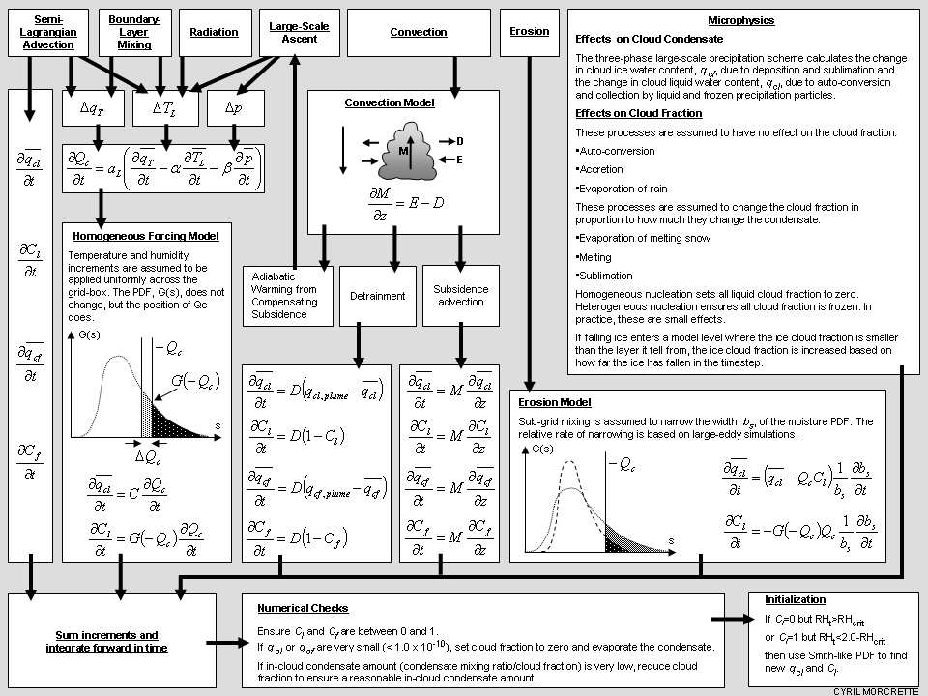
\includegraphics[scale=1.0]{pc2_process_explanation} 
\caption{Schematic summary of the PC2 cloud scheme.} 
\label{fig:schematic} 
\end{center} 
\end{figure} 

\begin{figure} 
\begin{center}

\includegraphics[scale=0.6]{Timestepping_ctl66.epsi}
\caption{Timestepping diagram for the control (non-PC2) scheme}
\label{fig:tstep_diag}
\end{center}
\end{figure}

\begin{figure}
\begin{center}

\includegraphics[scale=0.6]{Timestepping_pc266.epsi}
\caption{Timestepping diagram for the PC2 scheme}
\label{fig:tstep_prog}
\end{center}
\end{figure}

\bibliography{refs} 
\bibliographystyle{plainnat}

\end{document}
